%*********************************
%Format telah disesuaikan sesuai *
%Panduan penulisan               *
%Disertasi Dan Tesis ITS         *
%*********************************
\documentclass[12pt, a4paper, twoside, bahasa]{report}
%\documentclass[12pt, a4paper,twoside]{report}

\title{Buku Tesis}
% Jika pakai windows untuk run
%    pertama kali dan error.
% Mohon cek miktex console jika 
%    compiler latex nya menggunakan miktex.
%------------------------------
%%%%%%%%%%%%%%%%%%%%%%%%%%%%%%%%%%%%%%%%%%%%
% FILE INI JANGAN DI UBAH
%%%%%%%%%%%%%%%%%%%%%%%%%%%%%%%%%%%%%%%%%%%%
%\usepackage[indonesian]{babel}
\usepackage[american]{babel}
%\usepackage[indonesian]{babel}
\usepackage[table,xcdraw]{xcolor}


\usepackage[pdfauthor={Nur Afandi},bookmarksnumbered,pdfborder={0 0 0}]{hyperref}
\usepackage[ruled,lined,commentsnumbered,linesnumbered]{algorithm2e}
\usepackage[utf8]{inputenc}
\usepackage{graphicx}
\usepackage{lipsum}
\usepackage{hyphenat}
\usepackage{rotating}
\usepackage{booktabs}
\usepackage{lscape}
%\usepackage{algpseudocode}
\usepackage[ruled,lined,commentsnumbered,linesnumbered]{algorithm2e}
\usepackage{algpseudocode}
\usepackage{makeidx}
\usepackage{rotating}
\makeindex
\usepackage{epsfig}
\usepackage{subfig}
\usepackage{pdflscape}
\usepackage[doublespacing]{setspace}
\setstretch{1.5}
\usepackage{type1cm}
\usepackage{longtable}
\usepackage{lscape}
\usepackage{lettrine}
\usepackage{hyperref}
\usepackage[pageref]{backref}
\usepackage{multirow}
\usepackage[table,xcdraw]{xcolor}
\usepackage{eso-pic}
\newcommand\BackgroundIm{
	\put(0,0){
		\parbox[b][\paperheight]{\paperwidth}{%
			\vfill
			\centering
			\includegraphics[height=\paperheight,
				keepaspectratio]{./lib/background.png}%
			\vfill
		}}}

\usepackage{fancyhdr} % Untuk pengaturan header dan footer yang lebih kompleks
\usepackage{etoolbox} % Untuk melakukan perubahan (patch) command internal LaTeX
\usepackage{url}
\usepackage{longtable}
\usepackage{float}
\usepackage{morefloats}
\floatstyle{boxed}
\newfloat{program}{thp}{lop}
\floatname{program}{Program}
\usepackage[fleqn]{amsmath}
\usepackage{nccmath}
\usepackage{enumitem}
\usepackage{ulem}
\usepackage[final]{pdfpages}
\usepackage{titlesec}
\usepackage{array}
\usepackage{multicol}
\usepackage{listings}
\usepackage{wrapfig}
\usepackage{array,tabularx}
\usepackage{lscape}
\usepackage{longtable}
\usepackage{caption}
\usepackage[export]{adjustbox}
\usepackage{ragged2e}
\usepackage{epsfig}
\usepackage{subfig}
\usepackage[top=35mm,left=40mm,right=30mm,bottom=30mm]{geometry}
\usepackage{pdflscape}
\usepackage[doublespacing]{setspace}
\setstretch{1.5}
\usepackage{type1cm}
\usepackage{lettrine}
\usepackage{hyperref}
\usepackage[pageref]{backref}
\usepackage{multirow}
\usepackage[table,xcdraw]{xcolor}
\usepackage{fancyhdr} % Untuk pengaturan header dan footer yang lebih kompleks
\usepackage{etoolbox} % Untuk melakukan perubahan (patch) command internal LaTeX
\usepackage{url}
\usepackage{longtable}
\usepackage{float}
\usepackage{morefloats}
\floatstyle{boxed}
\newfloat{program}{thp}{lop}
\floatname{program}{Program}
\usepackage[fleqn]{amsmath}
\usepackage{enumitem}
\usepackage{ulem}
\usepackage[final]{pdfpages}
\usepackage{titlesec}
\usepackage{array}
\usepackage{multicol}
\usepackage{listings}
\usepackage{wrapfig}
\usepackage{array,tabularx}
\usepackage{longtable}
\usepackage{caption}
%\usepackage{natbib}
%\usepackage[numbers]{natbib}
\usepackage[numbers]{natbib}
\usepackage{siunitx}
\usepackage{dirtree}
\usepackage{hyperref}
\usepackage{adjustbox}

%\usepackage[sorting=none]{biblatex}

%square,sort,comma,numbers

%\renewcommand{\uline}[1]{\textit{#1}}
%\bibliographystyle{apalike}
\usepackage[export]{adjustbox}
\usepackage{ragged2e}
\usepackage[utf8]{inputenc}
\usepackage{afterpage}
\usepackage{lipsum}
%\usepackage{cite}
% More tidy url
%\usepackage{url}
%\usepackage{breakurl}
%\def\UrlBreaks{\do\/\do-\do.}

% Set paper size and margin
\usepackage{geometry}
\geometry{
	a4paper,
	left=40mm,
	top=35mm,
	right=30mm,
	bottom=30mm,
}

% untuk Cover
\newenvironment{FontCover}{\fontfamily{phv}\selectfont}{\par}
% untuk Lembar Pengesahan
\newenvironment{Kondisi}
{\par\vspace{\abovedisplayskip}\noindent
\tabularx{\columnwidth}{>{$}l<{$} @{${}:{}$} >{\raggedright\arraybackslash}X}}
	{\endtabularx\par\vspace{\belowdisplayskip}}
	\newenvironment{Kondisi2}
	{\par\vspace{\abovedisplayskip}\noindent
	\tabularx{\columnwidth}{>{$}l<{$} @{${}:{}$} >{\raggedright\arraybackslash}X}}
{\endtabularx\par\vspace{\belowdisplayskip}}
% Line spacing
\linespread{1.5}

% fix titlesec bug
\makeatletter
\patchcmd{\ttlh@hang}{\parindent\z@}{\parindent\z@\leavevmode}{}{}
\patchcmd{\ttlh@hang}{\noindent}{}{}{}
\makeatother

% Pengaturan format Chapter dan Section
\titleformat{\chapter}[display]{\bfseries\Large}{BAB \centering\thechapter}{0ex}{\vspace{0ex}\centering}[\vspace{3ex}]
\titlespacing*{\chapter}{0pt}{-4ex}{0pt}
\titleformat{\section}{\bfseries\normalsize}{\MakeUppercase{\thesection}}{1ex}{}
\titleformat{\subsection}{\normalsize\bfseries}
\titleformat{\subsubsection}{\normalsize\bfseries}

\titlespacing{\section}{0pt}{0pt}{1ex}
\titlespacing{\subsection}{0pt}{0pt}{1ex}
\titlespacing{\subsubsection}{0pt}{0pt}{1ex}

% Keterangan rumus
\newenvironment{conditions}
{\par\vspace{\abovedisplayskip}\noindent
\tabularx{\columnwidth}{>{$}l<{$} @{${}={}$} >{\raggedright\arraybackslash}X}}
{\endtabularx\par\vspace{\belowdisplayskip}}

% Caption label bold
\usepackage[labelfont=bf]{caption}
\captionsetup{labelfont=bf}

% Jarak caption dengan obyek
\captionsetup[figure]{font=small,skip=15pt}
\captionsetup[table]{font=small,skip=15pt}


\DeclareCaptionLabelSeparator{none}{}
\captionsetup{labelsep=period}
% Caption nama
\renewcommand{\figurename}{Gambar}
\renewcommand{\tablename}{Tabel}
\renewcommand{\lstlistingname}{Kode}

% Cek nomor halaman
\usepackage{changepage}

% Cek spelling
\usepackage{lipsum}
\setcounter{secnumdepth}{5}
\hyphenation{meng-gerak-kan mem-per-kenal-kan pe-ri-la-ku di-je-las-kan mem-bu-tuh-kan me-ne-rap-kan}

% Definisi untuk "halaman sengaja dikosongkan"
\def\kosong{
	\vspace*{\fill}
	\begin{center}\textit{This page is intentionally left blank}\end{center}
	\vfill
}

% Halaman sengaja dikosongkan
\patchcmd{\cleardoublepage}{\hbox{}}{\kosong}{}{}
% Untuk citation
%\newcommand{\tab}[1]{\hspace{.2\textwidth}\rlap{#1}}
\renewcommand*{\backreflastsep}{, }
\renewcommand*{\backreftwosep}{, }
\renewcommand*{\backref}[1]{}
%\renewcommand*{\backrefalt}[4]{
%	\ifcase #1
%	No citations.
%	\or
%	(Dikutip pada halaman #2).
%	\else
%	(Dikutip pada halaman #2).
%	\fi
%}
% Pengaturan penomoran halaman menggunakan package fancyhdr
\fancyhf{} 								% Mengosongkan header dan footer
\renewcommand{\headrulewidth}{0pt} 		% Menghapus garis horizontal pada header
\pagestyle{fancy} 						% Mengubah pagestyle dokumen menjadi fancy
\fancyfoot[CE,CO]{\thepage}				% Footer kanan pada hal. ganjil dan sebaliknya
%\patchcmd{\chapter}{plain}{fancy}{}{} 	% Mengubah pagestyle pada chapter menjadi fancy
\patchcmd{\chapter}{empty}{plain}{}{}
\usepackage{ifthen}
\newboolean{PembimbingDua}
\setboolean{PembimbingDua}{false}
\newboolean{bThesis}
\setboolean{bThesis}{true}

%\newcommand{\Tesis}
%{	\setboolean{bThesis}{true}
%}



\newboolean{PembimbingTiga}
\setboolean{PembimbingTiga}{false}

\newboolean{PengujiTiga}
\setboolean{PengujiTiga}{false}

\newboolean{PengujiEmpat}
\setboolean{PengujiEmpat}{false}

\newboolean{Nomenklatur}
\setboolean{Nomenklatur}{false}

\newboolean{bDoktor}
\setboolean{bDoktor}{false}
\newboolean{bMaster}
\setboolean{bMaster}{false}

\renewcommand{\em}[1]{\textit{#1}}
\renewcommand{\emph}[1]{\textit{#1}}

\newcommand{\Mahasiswa}[2]{
	\newcommand{\NamaMahasiswa}{#1}
	\newcommand{\NrpMahasiswa}{#2}
}
\newcommand{\PembimbingSatu}[2]
{
	\newcommand{\PbSatu}{#1}
	\newcommand{\NipPbSatu}{#2}
}
\newcommand{\PembimbingDua}[2]{
	\setboolean{PembimbingDua}{true}
	\newcommand{\PbDua}{#1}
	\newcommand{\NipPbDua}{#2}
}

\newcommand{\PembimbingTiga}[2]{
	\setboolean{PembimbingTiga}{true}
	\newcommand{\PbTiga}{#1}
	\newcommand{\NipPbTiga}{#2}
}

\newcommand{\PengujiSatu}[2]
{
	\newcommand{\PjSatu}{#1}
	\newcommand{\NipPjSatu}{#2}
}
\newcommand{\PengujiDua}[2]
{	\newcommand{\PjDua}{#1}
	\newcommand{\NipPjDua}{#2}
}
\newcommand{\PengujiTiga}[2]
{
	\setboolean{PengujiTiga}{true}
	\newcommand{\PjTiga}{#1}
	\newcommand{\NipPjTiga}{#2}
}

\newcommand{\PengujiEmpat}[2]
{
	\setboolean{PengujiEmpat}{true}
	\newcommand{\PjEmpat}{#1}
	\newcommand{\NipPjEmpat}{#2}
}
\newcommand{\KaDep}[2]
{
	\newcommand{\NmKaDep}{#1}
	\newcommand{\NipKaDep}{#2}
}
\newcommand{\CoverFooter}[1]
{\newcommand{\bdk}{#1}
}
\newcommand{\Judul}[1]
{
	\newcommand{\JdTesis}{#1}
}
\newcommand{\TanggalUjian}[1]
{
	\newcommand{\TglUjian}{#1}
}
\newcommand{\PeriodeWisuda}[1]
{
	\newcommand{\PerWisuda}{#1}
}

\newcommand{\Fakultas}[1]
{
	\newcommand{\fak}{#1}
}
\newcommand{\BeltFakultas}[1]
{
	\newcommand{\bbelt}{#1}
}
\newcommand{\Departemen}[1]
{
	\newcommand{\Dep}{#1}
}
\newcommand{\ggGelar}{xxxx}
\newcommand{\pPengesahan}{xxxxxxxx}

\newcommand{\Gelar}[1]
{
	\renewcommand{\ggGelar}{#1}
}

\newcommand{\tsss}{Disertasi disusun untuk memenuhi salah satu syarat memperoleh gelar}

\newcommand{\Disertasi}[1]
{\renewcommand{\tsss}{Disertasi disusun untuk memenuhi salah satu syarat memperoleh gelar}
	\renewcommand{\pPengesahan}{LEMBAR PENGESAHAN DISERTASI}
	\renewcommand{\ggGelar}{#1}
	\setboolean{bMaster}{false}
	\setboolean{bThesis}{true}
}

\newcommand{\prop}{PROPOSAL DISERTASI}
\newcommand{\ProposalDisertasi}
{	\renewcommand{\prop}{PROPOSAL DISERTASI}
	\setboolean{bMaster}{false}
	\setboolean{bThesis}{false}
}

\newcommand{\Tesis}[1]
{
	\renewcommand{\tsss}{The thesis is written to fulfill one of the requirements for obtaining a degree
		of}
	\renewcommand{\pPengesahan}{THESIS VALIDATION SHEET}
	\setboolean{bMaster}{true}
	\setboolean{bThesis}{true}
	\renewcommand{\ggGelar}{#1}

}

\newcommand{\ProposalTesis}
{	\setboolean{bMaster}{true}
	\renewcommand{\prop}{THESIS PROPOSAL}
	\setboolean{bThesis}{false}
}


\newboolean{JudulTesisEng}
\setboolean{JudulTesisEng}{true}

\newcommand{\JudulEng}[1]
{
	\setboolean{JudulTesisEng}{true}
	\newcommand{\JdTesisEng}{#1}
}

\newcommand{\Kode}[1]
{\newcommand{\Kodekk}{#1}
}

\newcommand{\TempatUjian}[1]
{
	\newcommand{\bTempatUjian}{#1}
}

\newcommand{\HariUjian}[1]
{
	\newcommand{\bHariUjian}{#1}
}

\newcommand{\DaftarRiwayatHidup}{
\addcontentsline{toc}{chapter}{Author Biography}
\titlespacing*{\chapter}{0pt}{0ex}{5ex}
\appendix
\chapter*{AUTHOR BIOGRAPHY}
%*********************************
%Gambar Foto 
\begin{center}
	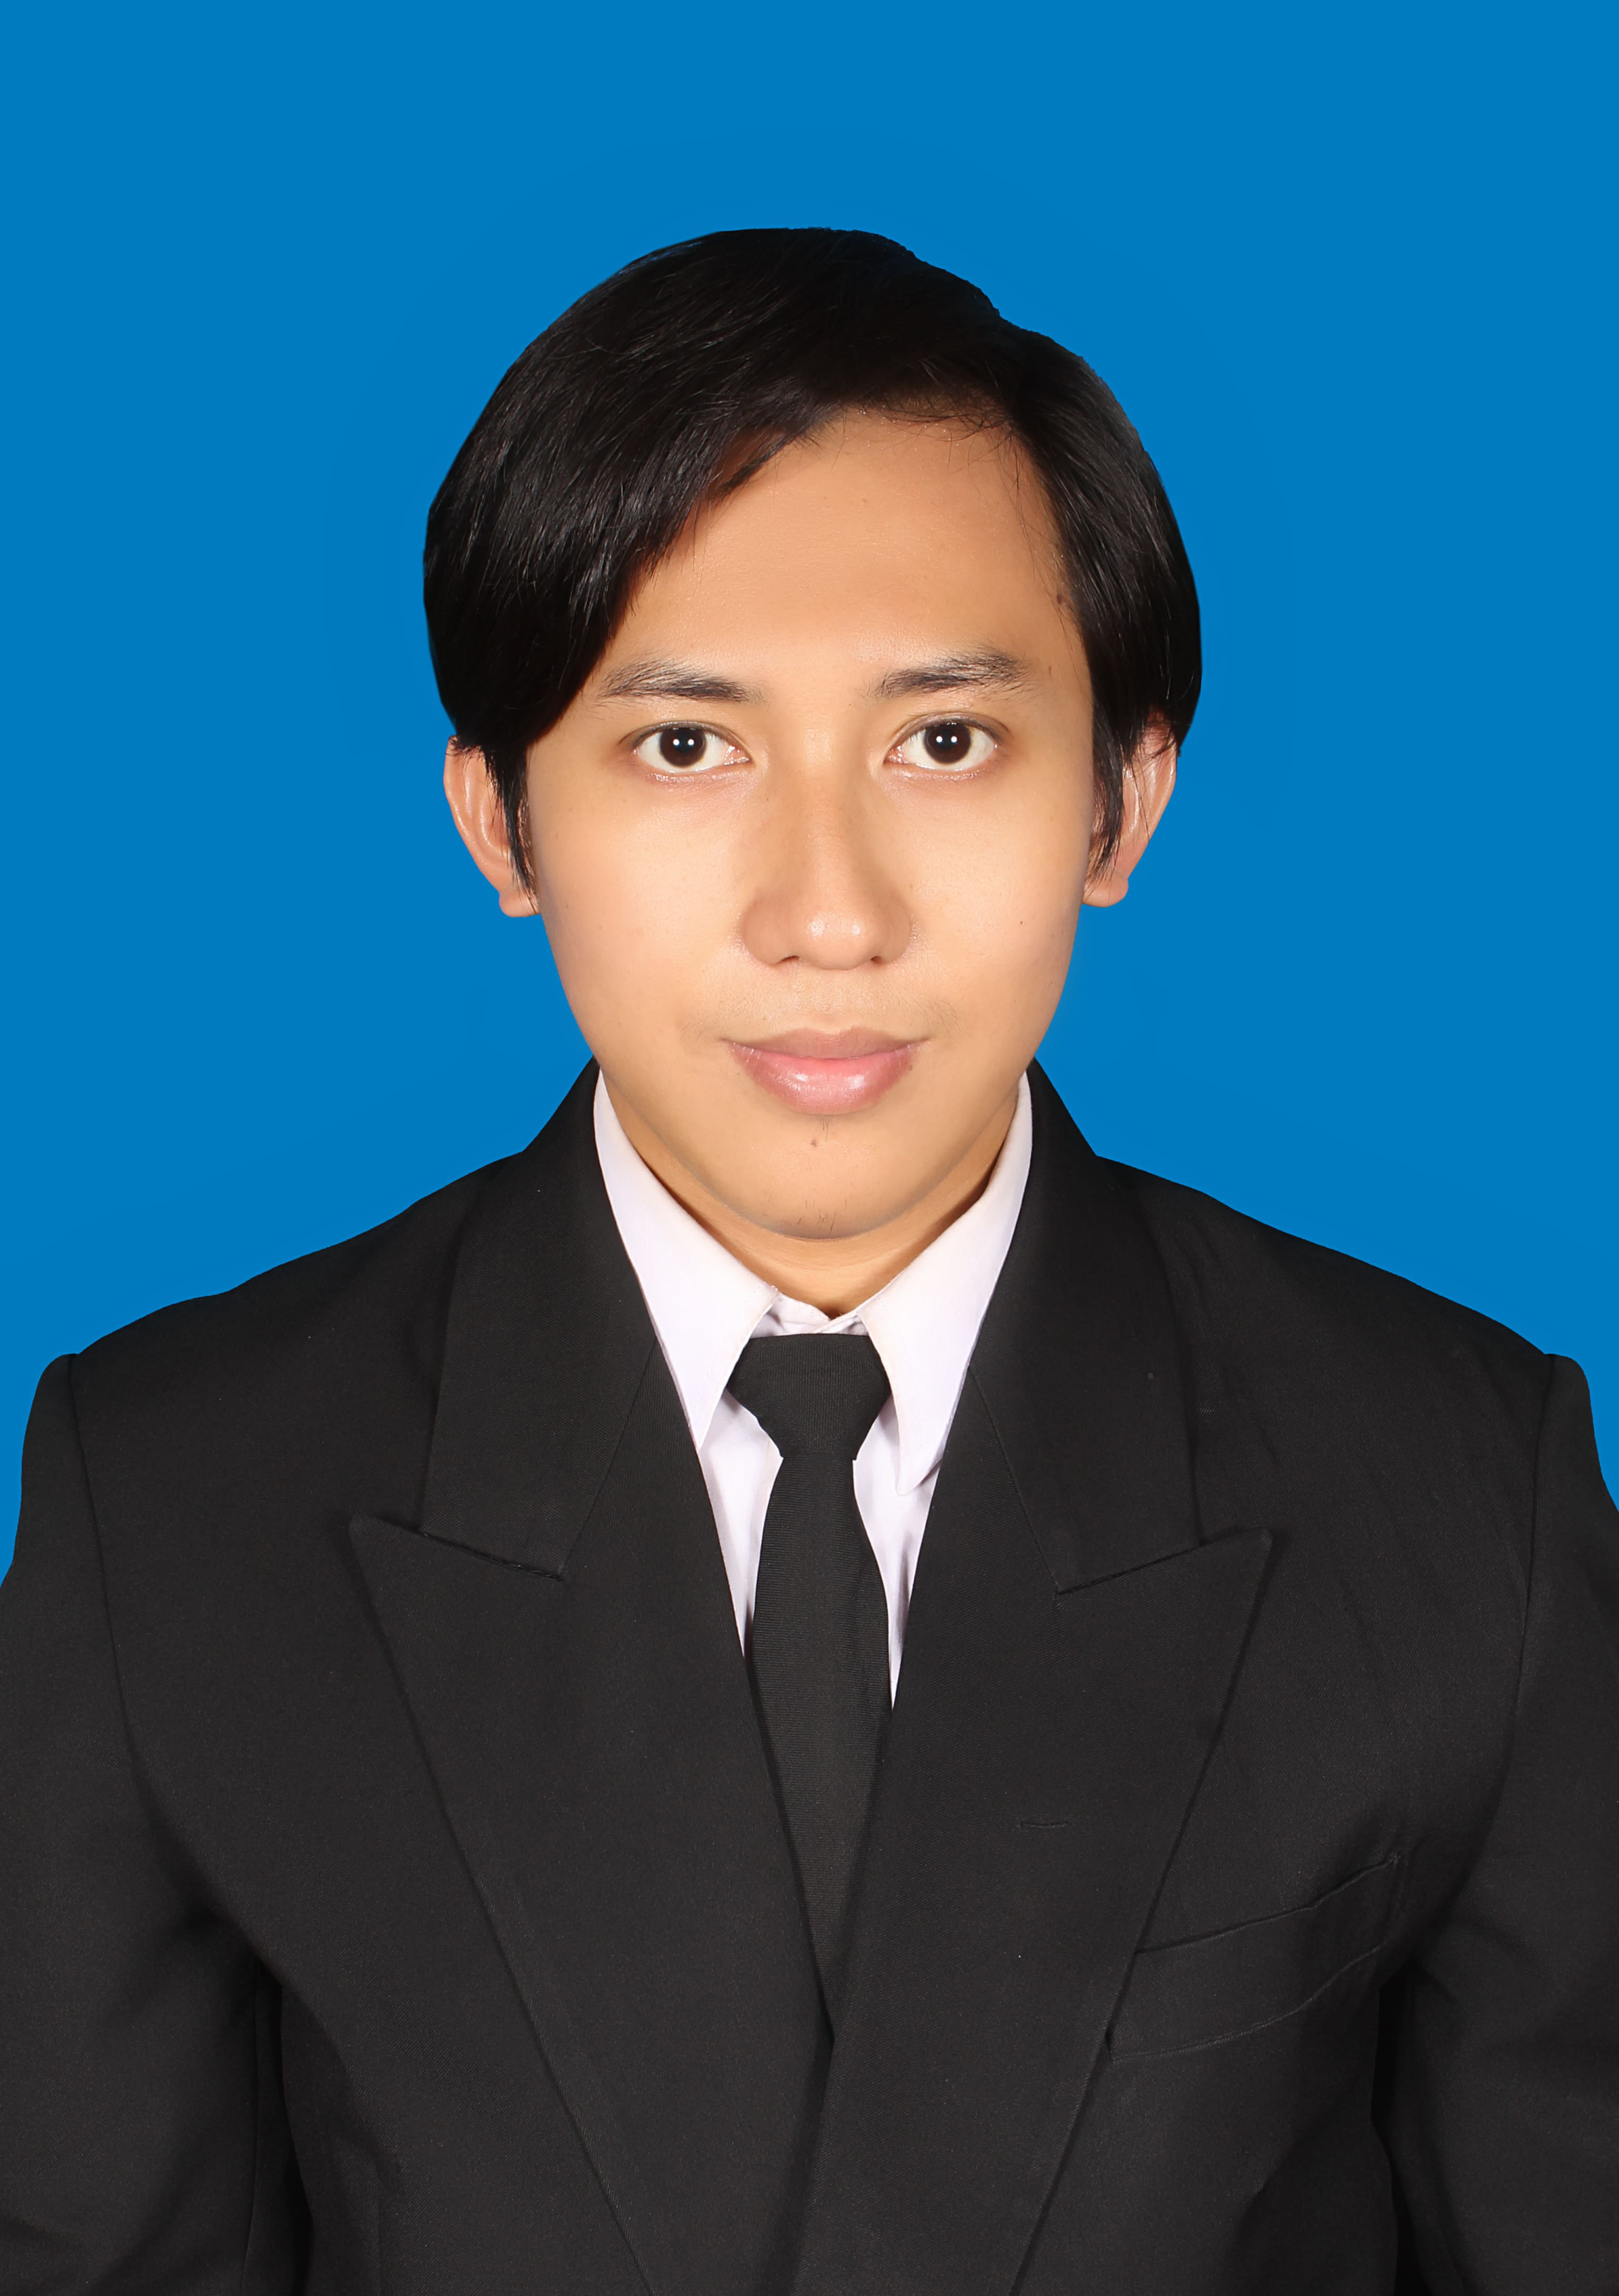
\includegraphics[height=0.2\textheight]{./ubah/foto_amik.jpg}
\end{center}
%*********************************
\section*{Personal Identity}
\begin{tabular}{p{3cm}cp{9cm}}
	%Masukan Identitas Disini.............
	Nama          & : &
	Amik Rafly Azmi Ulya                           \\
	Tempat Lahir  & : &
	Jepara                                         \\
	Tanggal Lahir & : &
	14 November 1999                               \\
	Alamat        & : &
	Mangkuyudan, Kartasura, Sukoharjo, Jawa Tengah \\
\end{tabular}

\section*{Educational Background}
\begin{tabular}{p{3cm}cp{9cm}}
	2022-2024 & : &
	Master Degree (S2), Department of Electrical Engineering, Faculty of Intelligent Electrical and Informatics Technology, Institut Teknologi Sepuluh Nopember \\
	          &   &                                                                                                                                             \\
	2018-2022 & : &
	Bachelor Degree (S1), Departement of Physics, Faculty of Science and Data Analytics, Institut Teknologi Sepuluh Nopember                                    \\
	          &   &                                                                                                                                             \\
	2015-2018 & : &
	2\textsuperscript{nd} Kudus Islamic State Senior High School (MAN)                                                                                          \\
	          &   &                                                                                                                                             \\
	2012-2015 & : &
	Unggulan Pondok Modern Selamat Junior High School (SMP)                                                                                                     \\
	          &   &                                                                                                                                             \\
	2006-2012 & : &
	Al-Islam Kartasura Islamic Elementary School (MI)                                                                                                           \\
\end{tabular}


\section*{Publication List}

\begin{enumerate}
	\item Amik Rafly Azmi Ulya et al. “HiroPoseEstimation: A Dataset of Pose Estimation for Kid-Size Humanoid Robot”. In: Journal of Information Technology and Computer Science 8.3 (2023), 231–240. DOI: 10.25126/ jitecs.202383568. URL: https://jitecs.ub.ac.id/index.php/ jitecs/article/view/568.
\end{enumerate}

% \section*{Riwayat Penelitian}
% \begin{enumerate}
% 	\item \lipsum[3]
% 	\item \lipsum[3]
% 	\item Penelitian Ke Tiga
% 	\item Penelitian Ke Empat
% \end{enumerate}
% \section*{Riwayat Lainnya}

% \lipsum[1]
\cleardoublepage}


\newcommand{\DaftarPustaka}{%\\renewcommand\bibname{Daftar Pustaka}
%\\addcontentsline{toc}{chapter}{\bibname}
%\\titlespacing*{\chapter}{0pt}{0ex}{5ex}
%\\appendix
%\%\bibliographystyle{apalike}
%\%\bibliographystyle{ieetr}
%\%\bibliographystyle{IEEEtranN}
%\\bibliographystyle{plainnat}
%\\bibliography{./ubah/pustaka}
%\\cleardoublepage
%\gdef \bibname{Daftar Pustaka}
\renewcommand \bibname {Bibliography}
\addcontentsline{toc}{chapter}{\bibname}
\titlespacing*{\chapter}{0pt}{0ex}{5ex}
\appendix
%\bibliographystyle{IEEEtranN}
\bibliographystyle{IEEEtran}
\bibliography{IEEEabrv,./ubah/pustaka.bib}
%\bibliography{IEEEabrv,pustaka.bib}
%\bibliography{../ubah/pustaka.bib}
%\bibliography{library}
\cleardoublepage}

\tolerance=9999
\emergencystretch=10pt
\hyphenpenalty=10000
\exhyphenpenalty=100



%************************************
% 1. JENIS BUKU
%    Pilih Salah Satu 
%************************************
%   \ProposalDisertasi
%   \ProposalTesis 
	\Tesis{Magister Teknik (MT)}
%	\Disertasi{Doktor (Dr)}
%***************************

%\ProposalDisertasi
%\ProposalTesis 
%\Tesis{Magister Teknik (MT)}
%\Disertasi{Doktor (Dr)}


%*******************************
%2.  Tulislah Kode Yang Sesuai 
%*******************************
%\Kode{DISERTASI - EE186601}
\Kode{THESIS - EE235401}
%\Kode{Proposal Tesis}
% \Kode{Thesis Proposal}
%\Kode{Proposal Disertasi}
%*******************************

%*******************************
%  3. Judul Proposal, Tesis atau 
%     Disertasi 
%     dipilih Salah Satu 
%-------------------------------
% Tulislah Judul Dalam Bahasa Indonesia
\Judul{Klasifikasi Aktivitas Kebugaran Lansia Berdasarkan Estimasi Pose Menggunakan Deep Learning}
% Tulislah Judul Dalam Bahasa Inggris
\JudulEng{Classification of Elderly Exercise Activity Based on Pose Estimation Using Deep Learning}
%***********************************
% 4. Identitas Mahasiswa
% Format :\Mahasiswa{Nama}{Nrp}
%------------------------------------
\Mahasiswa{Amik Rafly Azmi Ulya}{6022221057}
%************************************
% 5. Waktu Dan Ruang Ujian
%------------------------------------
%Tanggal Ujian 
\TanggalUjian{July 8, 2024}
% Perioda wisuda  
\PeriodeWisuda{September 2024} 
%Hari ujian dan Tempat Ujian 
\HariUjian{Monday}
\TempatUjian{B-211 Room}


%************************************
%6. Identitas Pembimbing 
%   Maximal Tiga Pembimbing
%   Format : \PembimbingXXX{Nama}{Nip}
%-----------------------------------
%\scalebox{.95}[1.0]{xxx}
\PembimbingSatu{Prof. Dr. Ir. Mauridhi Hery Purnomo, M.Eng.}{195809161986011001}
\PembimbingDua{Dr. Eko Mulyanto Yuniarno, S.T., M.T.}{196806011995121009}
%\PembimbingTiga{Reza Fuad Rachmadi, S.T., M.T., Ph.D}{198504032012121000}

%************************************
% 7. Identitas Penguji 
%     Maximal 4 penguji
%     Format : \PengujiXXX{Nama}{Nip}
%-------------------------
\PengujiSatu{Dr. Diah Puspito Wulandari, S.T., M.Sc.}{198012192005012001}
\PengujiDua{Dr. Surya Sumpeno, S.T., M.Sc.}{1996912091997031002}
\PengujiTiga{Dr. Arief Kurniawan, S.T., M.T.}{1197409072002121001}
%\PengujiEmpat{-}{-}

%************************************
% 8. Identitas Fakultas ------------------------------------
\Fakultas{Fakultas Teknologi Elektro Dan Informatika Cerdas}
\BeltFakultas{BeltFte}
%************************************
% 9. Identitas Departement
%-----------------------------------
\Departemen{Teknik Elektro}

\KaDep{Dedet Candra Riawan, S.T., M.Eng., Ph.D}{197311192000031001}
%***********************************
% 10. Footer Identitas Program Studi 
%  Pada Cover
%----------------------------------
\CoverFooter{\normalsize
MASTER PROGRAM\\
	MULTIMEDIA INTELLIGENT NETWORK\\
	DEPARTMENT OF ELECTRICAL ENGINEERING\\
	\makebox[0.95\textwidth][l]{FACULTY OF INTELLIGENT ELECTRICAL AND INFORMATICS TECHNOLOGY}\\
	INSTITUT TEKNOLOGI SEPULUH NOPEMBER\\
	SURABAYA\\
	2024}

%**********************************
%File Penting Yang Dapat di Edit:
%**********************************
%Abstrak :
%        ->\ubah\abstrak.tex
%Abstrak Bhs Inggris :
%        ->\ubah\abstrakEng.tex
%Kata Penggantar :
%        ->\ubah\pengantar.tex 
%Nomenklatur :
%        ->\ubah\Nomenklatur.tex
%Database Daftar Pustaka
%        ->\ubah\pustaka.bib
%DaftarRiwayatHidup 
%        ->\ubah\DaftarRiwayatHidup.tex
%----------------------------------
%**********************************
%Dokumen Utama
%----------------------------------
\begin{document}
%%%%%%%%%%%%%%%%%%%%%%%%%%%%%%%%%%%%%%%%%%%%
% FILE INI JANGAN DI UBAH ATAU MODIFIKASI
%%%%%%%%%%%%%%%%%%%%%%%%%%%%%%%%%%%%%%%%%%%%
\normalsize
\pagenumbering{roman}
\singlespacing
\hyphenpenalty=1000
\tolerance=1000
\emergencystretch=2.5em
% Cover
%\addcontentsline{toc}{chapter}{Cover}
\begin{FontCover}
	\sffamily	
\thispagestyle{empty}
\begin{figure} [!t]
	
\includegraphics[keepaspectratio=true,scale=1,left]{./lib/LogoITS.png}
	\caption*{}
	\label{fig:LogoITS}
\end{figure}
\vspace{1ex}
%\noindent\makebox[\linewidth]{\rule{\paperwidth}{10pt}}
\makebox[\linewidth]{\includegraphics[keepaspectratio=true,width=\paperwidth]{./lib/\bbelt}}
\vspace{10ex}
\justify
\textbf{\Kodekk}
\vspace{1ex}
\justify
\Large
\begin{spacing}{1}
%Masukan Judul Tesis Disini
\flushleft
\textbf{\JdTesisEng}
\end{spacing}
\normalsize
\vfill
\justify

%\begin{spacing}{1}
\large
\MakeUppercase{\NamaMahasiswa}\\
NRP  \uppercase{\NrpMahasiswa}
\vspace{2ex}
\justify
\normalsize

\ifthenelse{\boolean{bMaster}}{\textbf{SUPERVISOR}}{\textbf{PROMOTOR}}\\
\PbSatu\\
\ifthenelse{\boolean{PembimbingDua}}{\ifthenelse{\boolean{bMaster}}{}{\\\textbf{Co.PROMOTOR\\}}}{}
\ifthenelse{\boolean{PembimbingDua}}{\PbDua\\}{}
\ifthenelse{\boolean{PembimbingTiga}}{\PbTiga\\}{}
 
\vfill
\justify
\bdk
\vspace{1ex}
%\rmfamily
\normalfont
\end{FontCover}
\newpage
\cleardoublepage
% Lembar pengesahan
\addcontentsline{toc}{chapter}{VALIDATION SHEET}
\ifthenelse{\boolean{bThesis}}
{ \AddToShipoutPicture*{\BackgroundIm}
	\begin{center}

		\Large\textbf{\pPengesahan}
		%\Large\textbf{PROPOSAL TESIS}
	\end{center}
	\begin{center}
		\tsss\\
		\textbf{\ggGelar}\\
		at\\
		\textbf{Institut Teknologi Sepuluh Nopember}\\
		\vspace{1ex}
		By:\\
		\textbf{\NamaMahasiswa}\\
		\textbf{NRP: \NrpMahasiswa}\\
		\vspace{1ex}
		Examination Date : \TglUjian\\
		Graduation Period : \PerWisuda\\
		\vspace{1ex}
	\end{center}
	\begin{center}
		Approved by:\\
		\textbf{Supervisor}:
	\end{center}
	\begin{enumerate}
		\item \PbSatu \hfill ...............................\\
		      NIP:\NipPbSatu \vfill
		      \ifthenelse{\boolean{PembimbingDua}}{\item \PbDua\hfill ...............................\\
		      NIP:\NipPbDua}\vfill
		      \ifthenelse{\boolean{PembimbingTiga}}{\item \PbTiga \hfill ...............................\\
		      NIP:\NipPbTiga}{}
	\end{enumerate}
	\begin{center}
		\textbf{Examiner}:
	\end{center}
	\begin{enumerate}
		\item \PjSatu \hfill ...............................\\
		      NIP:\NipPjSatu
		      \vfill
		\item \PjDua \hfill ...............................\\
		      NIP:\NipPjDua\vfill
		      \ifthenelse{\boolean{PengujiTiga}}{
		\item \PjTiga \hfill ...............................\\NIP:\NipPjTiga\vfill}{}
		      \ifthenelse{\boolean{PengujiEmpat}}{
		\item \PjEmpat \hfill ...............................\\ NIP:\NipPjEmpat\vfill}{}
	\end{enumerate}
	\vfill
	\begin{center}
		Head of \Dep \\
		\fak\\
		\vspace{9ex}
		\underline{\NmKaDep}\\
		NIP:\NipKaDep
	\end{center}
	\newpage
}
{
	\begin{center}
		\textbf{VALIDATION SHEET\\
			THESIS PROPOSAL}\\
	\end{center}
	\vspace{5ex}
	\begin{tabular}{p{2cm} c p{8cm}}
		Title & : & \JdTesisEng    \\
		By    & : & \NamaMahasiswa \\
		Nrp   & : & \NrpMahasiswa
	\end{tabular}
	\vspace{5ex}
	\begin{center}
		\textbf{Has Been Examined On}
	\end{center}
	\begin{tabular}{p{2cm} c p{8cm}}
		Day   & : & \bHariUjian   \\
		Date  & : & \TglUjian     \\
		Place & : & \bTempatUjian
	\end{tabular}
	\vspace{5ex}
	%\scalebox{.95}[1.0]{\PjSatu}

	\begin{tabular}{p{8cm} p{8cm} }
		\textbf{Examiner}                        & \textbf{Supervisor Candidate} \\
		\vspace{8ex}\hspace{-10ex}1. \PjSatu     &
		\vspace{8ex}\hspace{-8ex}1. \PbSatu                                      \\
		\hspace{-7ex}Nip :\NipPjSatu             &
		\hspace{-5ex}Nip :\NipPbSatu                                             \\
		\vspace{8ex}\hspace{-10ex}2. \PjDua      &
		\ifthenelse{\boolean{PembimbingDua}}
		{\vspace{8ex}\hspace{-8ex}2. \PbDua}{}                                   \\
		\hspace{-7ex}Nip :\NipPjDua              &
		\ifthenelse{\boolean{PembimbingDua}}
		{\hspace{-5ex}Nip :\NipPbDua}{}                                          \\
		\ifthenelse{\boolean{PengujiTiga}}
		{\vspace{8ex}\hspace{-10ex}3. \PjTiga}{} &
		\ifthenelse{\boolean{PembimbingTiga}}
		{\vspace{8ex}\hspace{-8ex}3. \PbTiga}{}                                  \\
		\ifthenelse{\boolean{PengujiTiga}}
		{\hspace{-7ex}Nip :\NipPjTiga}{}         &
		\ifthenelse{\boolean{PembimbingTiga}}
		{\hspace{-5ex}Nip :\NipPbTiga}{}                                         \\


		\ifthenelse{\boolean{PengujiEmpat}}
		{\vspace{8ex}\hspace{-10ex}4. \PjTiga}{} &                               \\
		\ifthenelse{\boolean{PengujiEmpat}}
		{\hspace{-7ex}Nip :\NipPjEmpat}{}        &                               \\
	\end{tabular}
	\newpage
}
\cleardoublepage

\ifthenelse{\boolean{bThesis}}
{
	\ifthenelse{\boolean{bMaster}}
	{
		\chapter*{STATEMENT OF THE THESIS AUTHENTICY}
		\addcontentsline{toc}{chapter}{STATEMENT OF THE THESIS AUTHENTICY}


		\begin{spacing}{1.5}

			I hereby declare that the entire content of my thesis with the title of \textbf{\JdTesisEng} is truly the result of an independent intellectual work, completed without the use of unauthorized materials, and is not the work of another party which I acknowledge as my work.

			All references cited or referred to have been written in full in the bibliography. If it turns out that this statement is not true, I am willing to accept sanctions under applicable regulations.

			\hspace{35ex}Surabaya \today

			\vspace{10ex}

			\hspace{35ex}\underline{\NamaMahasiswa}

			\hspace{35ex}Nrp: \NrpMahasiswa

		\end{spacing}
		\cleardoublepage

	}
	{

		\chapter*{PERNYATAAN KEASLIAN DISERTASI}
		\addcontentsline{toc}{chapter}{PERNYATAAN KEASLIAN DISERTASI}

		\begin{spacing}{1.5}

			Dengan ini saya menyatakan bahwa isi keseluruhan Disertasi  saya dengan judul \textbf{\JdTesis} adalah benar-benar hasil karya intelektual mandiri, diselesaikan tanpa menggunakan bahan-bahan yang tidak diijinkan dan bukan merupakan karya pihak lain yang saya akui sebagai karya sendiri.

			Semua referensi yang dikutip maupun dirujuk telah ditulis secara lengkap pada daftar pustaka. Apabila ternyata pernyataan ini tidak benar, saya bersedia menerima sanksi sesuai peraturan yang berlaku.

			\vspace{2ex}

			\hspace{35ex}Surabaya %\today

			\vspace{10ex}

			\hspace{35ex}\underline{\NamaMahasiswa}

			\hspace{35ex}Nrp: \NrpMahasiswa

		\end{spacing}
		\cleardoublepage
	}
}{}




% Kata pengantar
\newpage

\addcontentsline{toc}{chapter}{PREFACE}
\begin{center}
	\Large\textbf{PREFACE}
\end{center}
\vspace{2ex}
%Tulis kata pengantar di sini
Praise and gratitude to the presence of Allah SWT. for all His grace, the author will able to work this research with the title \textbf{Classification of Elderly Exercise Activity Based on Pose Estimation Using Deep Learning}. This research was written as a requirement for completing a master’s degree at the Department of Electrical Engineering, Institut Teknologi Sepuluh Nopember.\\
The author also expresses great thanks to:
\begin{itemize}
	\item Parents and family for their encouragement and
	      support during the author’s study.
	\item Prof. Dr. Ir. Mauridhi Hery Purnomo, M.Eng. and Dr. Eko Mulyanto Yuniarno, ST. MT. as the supervising lecturer who has provided a lot of advice on this research.
	\item Nabila Shafa Oktavia who helped the author in technical and non-technical support.
	\item Friends from the B300 laboratory who always accompany and provide support in various forms of support.
	\item As well as friends from the class of 2022 who have passed the lecture period together with the author.
\end{itemize}
\vspace{26pt}
\begin{flushright}
	\begin{tabular}[b]{c}
		Surabaya, July 2024
		\\
		\\
		\\
		The Author
	\end{tabular}
\end{flushright}

\cleardoublepage
\newpage
% Abstrak
\begin{spacing}{1}
    \begin{center}
		\large\textbf{\JdTesisEng}
	\end{center}
	\normalsize
	\begin{adjustwidth}{-0.2cm}{}
		\begin{tabular}{lcp{0.9\linewidth}}
		By &:& \NamaMahasiswa\\
			Student Identity Number &:&\NrpMahasiswa\\
			Supervisor &:& 1. \PbSatu\\
			\ifthenelse{\boolean{PembimbingDua}}{& & 2. \PbDua\\}{}
			\ifthenelse{\boolean{PembimbingTiga}}{& & 3. \PbTiga\\}{}
		\end{tabular}
	\end{adjustwidth}
	\vspace{2ex}
	
	\begin{center}
		\Large\textbf{ABSTRACT}
	\end{center}
	\vspace{1ex}
    %Tulis Abstrak disini
    Older people's productivity often declines, especially in terms of physical ability. Physical decline can be slowed down with exercise and other physical activities. However, activities such as stretching are often neglected by the elderly. Exercise activities for the elderly are important so that the elderly can maintain their health in old age. Research on elderly activity recognition has been widely developed. Convolutional Neural Network (CNN) is a type of artificial neural network specifically designed for image processing and recognition. On the other hand, Long Time-Term Memory (LSTM) is an efficient method for solving real-time problems. These two methods can be used for labeling and recognizing physical activity movements in the elderly. Physical activities performed by the elderly need to be customized. In this study, we developed a model with elderly pose estimation. One of the frameworks for human pose estimation is Mediapipe Pose Estimation (MPE). Therefore, this research focuses on the recognition and detection of fitness movements in the elderly. The work begins with the acquisition of datasets in the form of exercise activities that have been adapted to the physical issues of the elderly. Data acquisition was carried out since there are few and limited datasets that discuss this training activity. The acquired video data was then subjected to a video frame extraction process. Each frame sequence represents the exercise activity information. Pose estimation has been done using the Mediapipe framework. The extraction results are then trained using CNN, LSTM, CNN-LSTM, and deep CNN-LSTM architectures. The accuracy of each model is 83.68\%, 92.89\%, 96.05\%, and 87.11\%. Based on these results, the CNN-LSTM model outperforms the other models with an accuracy rate of 96.05\%. The error in recognizing data patterns is shown using the loss metric. The loss value of the CNN-LSTM model is 0.1498, the smallest compared to other models. This value indicates the model's ability to predict data with the lowest error rate. In addition, in other metrics, this model outperforms other models. Precision, recall, and f1-score of the CNN-LSTM model are at 0.96, respectively.

    %Tulis Kata Kunci disini
    \vspace{2ex}
    \textbf{Keyword}: Activity, Deep Learning, Elderly, Pose Estimation
\end{spacing}
\cleardoublepage
\ifthenelse{\boolean{JudulTesisEng}}
{
	\begin{spacing}{1}
    \begin{center}
		\large\textbf{\JdTesis}
	\end{center}
	\normalsize
	\begin{adjustwidth}{-0.2cm}{}
		\ifthenelse{\boolean{bMaster}}{
		
		\begin{tabular}{lcp{0.9\linewidth}}
		Nama Mahasiswa &:& \NamaMahasiswa\\
			NRP &:&\NrpMahasiswa\\
			Pembimbing &:& 1. \PbSatu\\
			\ifthenelse{\boolean{PembimbingDua}}{& & 2. \PbDua\\}{}
			
			\ifthenelse{\boolean{PembimbingTiga}}{& & 3. \PbTiga\\}{}
			
			
			
		\end{tabular}
	}{
	\begin{tabular}{lcp{0.7\linewidth}}
		Nama Mahasiswa &:& \NamaMahasiswa\\
		NRP &:&\NrpMahasiswa\\
		Promotor &:&  \PbSatu\\
		\ifthenelse{\boolean{PembimbingTiga}}{
		\ifthenelse{\boolean{PembimbingDua}}{Co. Promotor&: & 1. \PbDua\\}{}
		\ifthenelse{\boolean{PembimbingTiga}}{& & 2. \PbTiga\\}{}
	}
{
	\ifthenelse{\boolean{PembimbingDua}}{\hspace{5ex}Co. Promotor&: & \PbDua\\}{}
	
}
	\end{tabular}

}

	
	\end{adjustwidth}
	\vspace{2ex}
	\begin{center}
		\Large\textbf{ABSTRAK}
	\end{center}
	\vspace{1ex}
    %Tulis Abstrak disini
    Produktivitas orang tua sering kali menurun, terutama dalam hal kemampuan fisik. Penurunan kemampuan fisik dapat diperlambat dengan olahraga dan aktivitas fisik lainnya. Namun, aktivitas seperti peregangan sering diabaikan oleh orang tua. Aktifitas latihan untuk elderly ini menjadi penting agar elderly dapat menjaga kesehatannya di usia lanjut. Riset mengenai pengenalan aktivitas lansia telah banyak dikembangkan. Convolutional Neural Network (CNN) adalah jenis jaringan saraf tiruan yang dirancang khusus untuk pengolahan dan pengenalan gambar. Di sisi lain, Long Shoert-Term Memory (LSTM) adalah metode yang efisien untuk memecahkan masalah real-time. Kedua metode ini dapat digunakan untuk pelabelan dan pengenalan gerakan aktivitas fisik pada lansia. Aktivitas fisik yang dilakukan oleh lansia perlu disesuaikan. Dalam penelitian ini, kami mengembangkan sebuah model dengan estimasi pose lansia. Salah satu kerangka kerja untuk estimasi pose manusia adalah Mediapipe Pose Estimation (MPE). Oleh karena itu, penelitian ini berfokus pada pengenalan dan deteksi gerakan kebugaran pada lansia. Pekerjaan diawali dengan akuisisi dataset berupa aktifitas latihan yang telah disesuaikan dengan isu-isu fisik para elderly. Akusisi data dilakukan sejak sedikit dan terbatasnya dataset yang membahas aktifitas latihan ini. Data video yang telah diakuisisi kemudian dilakukan proses ekstraksi video frame. Setiap urutan frame mewakili informasi aktifitas latihan. Estimasi pose telah dilakukan menggunakan framework Mediapipe. Hasil ekstraksi ini kemudian dilatih menggunakan arsitektur CNN, LSTM, CNN-LSTM, dan deep CNN-LSTM. Akurasi setiap model sebesar 83.68\%, 92.89\%, 96.05\%, dan 87.11\%. Berdasarkan hasil tersebut, model CNN-LSTM mengungguli model-model lainnya dengan tingkat akurasi 96.05\%. Kesalahan dalam mengenali pola data ditunjukkan menggunakan metric loss. Nilai loss model CNN-LSTM sebesar 0.1498, paling kecil dibandingkan dengan model-model lainnya. Nilai ini menunjukkan kemampuan model dalam memprediksi data dengan tingkat kesalahan paling rendah. Selain itu, pada metrcis lainnya, model ini mengungguli daripada model lainnya. Precision, recall, dan f1-score model CNN-LSTM berada pada nilai 0.96, masing-masing.

    %Tulis Kata Kunci disini
    \vspace{2ex}
    \textbf{Kata kunci }: Aktivitas, \textit{Deep Learning}, Lansia, Estimasi Pose

\end{spacing}
}{}
\cleardoublepage

% Daftar isi
\renewcommand*\contentsname{TABLE OF CONTENTS}
\titlespacing*{\chapter}{0pt}{0ex}{0ex}
\tableofcontents
\cleardoublepage
% Daftar gambar
\renewcommand*\listfigurename{LIST OF FIGURES}
\addcontentsline{toc}{chapter}{\listfigurename}
\titlespacing*{\chapter}{0pt}{0ex}{0ex}
\listoffigures
\cleardoublepage
% Daftar tabel
\renewcommand*\listtablename{LIST OF TABLES}
\addcontentsline{toc}{chapter}{\listtablename}
\titlespacing*{\chapter}{0pt}{0ex}{0ex}
\listoftables
\cleardoublepage
% Nomenklatur
\addcontentsline{toc}{chapter}{NOMENCLATURE} % kata pengantar
\begin{center}
	\Large\textbf{NOMENCLATURE}
\end{center}
\vspace{1ex}
\begin{tabular}{ll}
	$b$       & LSTM - bias                         \\
	Conv1D    & Convolutional 1 Dimension           \\
	CNN       & Convolution Neural Network          \\
	$C_t$     & LSTM - Cell State                   \\
	FC        & Fully Connected                     \\
	FN        & False Negative                      \\
	FP        & False Positive                      \\
	$f_t$     & LSTM - Forget Gate                  \\
	$h_t$     & LSTM - Hidden Outputs               \\
	$h_{t-1}$ & LSTM - Hidden State at $t$ - 1 time \\
	$i_t$     & LSTM - Input Gate                   \\
	LSTM      & Long Short Term Memory              \\
	NN        & Neural Networks                     \\
	$o_t$     & LSTM - Output Gate                  \\
	ReLU      & Rectified Linear Unit               \\
	RNN       & Recurrent Neural Networks           \\
	$\sigma$  & LSTM - Sigmoid Function             \\
	tanh      & LSTM - tanh Function                \\
	TN        & True Negative                       \\
	TP        & True Positive                       \\
	$V$       & Mediapipe - Keypoint Vector         \\
	W         & Weights                             \\
	$x_t$     & LSTM - Input at t time              \\
	$z_{max}$ & Mediapipe - Maximum Depth           \\
	$z_{min}$ & Mediapipe - Minimum Depth           \\

	% $s_i$            & Static Variables                                \\
	% $s^{2}$          & Sample Variance                                 \\
	% TFT              & Temporal Fusion Transformers                    \\
	% VSN              & Variable Selection Network                      \\
	% $\boldsymbol{v}$ & Attention - Value    							 \\
	% $W_H$            & Head Weight                                     \\
	% $W_K$            & Key Weight                                      \\
	% $W_Q$            & Query Weight                                    \\
	% $W_V$            & Value Weight                                    \\
\end{tabular}
\newpage

\cleardoublepage

% Bab isi buku
\titleformat{\chapter}[display]{\bfseries\Large}{CHAPTER \centering\thechapter}{0ex}{\vspace{0ex}\centering}[\vspace{0ex}]
\titleformat{\section}{\bfseries\large}{\MakeUppercase{\thesection}}{1ex}{}
\titleformat{\subsection}{\bfseries\large}{\MakeUppercase{\thesubsection}}{1ex}{}
\titleformat{\subsubsection}{\bfseries\large}{\MakeUppercase{\thesubsubsection}}{1ex}{}
\titlespacing*{\chapter}{0pt}{-4ex}{0pt}
\titlespacing{\section}{0pt}{0pt}{0pt}
\titlespacing{\subsection}{0pt}{0pt}{0pt}
\titlespacing{\subsubsection}{0pt}{0pt}{0pt}
% Indent paragraph
\setlength{\parindent}{0.8cm}
\begin{spacing}{1.5}
	
\begin{spacing}{1.2}
	\chapter{INTRODUCTION}
\end{spacing}


\pagenumbering{arabic}
\vspace{4ex}

\section{Background}
\label{sec1:Introduction}

% elderly secara umum
The global elderly population is experiencing unprecedented growth, and this trend is expected to continue into the foreseeable future. As of 2019, there were approximately 703 million individuals aged 65 or older worldwide, accounting for 9\% of the total global population \cite{nations2019world}. Projections indicate that this number will double by the year 2050, highlighting the increasing importance of addressing the needs of this demographic. One significant challenge faced by the elderly is a decline in productivity, particularly in terms of physical capabilities, which can greatly affect their independence and quality of life.

% penurunan kemampuan fisik elderly
The decline in physical capabilities among the elderly can be mitigated through regular exercise and physical activity. However, such activities are often neglected by the elderly due to various barriers, including lack of motivation, fear of injury and limited access to professional guidance. Exercise for the elderly requires special considerations, as their physical capacities differ significantly from those of younger, more productive individuals. Consequently, specialized exercise programs designed specifically for the elderly are essential. These programs often necessitate the assistance of physiotherapists or other trained professionals to ensure that exercises are performed safely and effectively.

% isu fisik yang sering menyerang
An elderly person can experience a variety of physical issues. Some physical issues that often affect elders are frozen shoulder \cite{FrozShoulder5}, tennis elbow \cite{TennisElbow3}, and knee pain \cite{KneePain5}. Adhesive Copsufitis, often known as frozen shoulder, is a painful condition in which the shoulder joint sustains damage without causing damage to the soft tissues. This type of injury affects 2-5\% of the population on average, with women accounting for 60\% of all injuries. According to recent research, people with diabetes have a five-fold increased risk of developing frozen shoulder in their 40s to 60s when compared to the general population. The shoulder joint's wide range of motion and heavy movement loads over it make it more prone to injury. This specific joint is dependent on the Deltoid Major, a large muscle, which is supported by the Cuff Rotators, a smaller set of muscles that are also essential for joint stability and muscular activity \cite{FrozShoulder6}.

Lateral epicondylitis or better known as tennis elbow is a condition that causes pain in the elbow due to inflammation of the tendons in the upper arm. This pain tends to be constant and causes disability in the elbow, especially the radio humeral joint which is known as lateral epicondylitis or lateral epicondylalgia. The disease often occurs due to repetitive activities involving the wrist and arm. The occurrence of this disease is also in line with a person's age. The disease affects the general population at about 1-3\% and increases sharply to 19\% in subjects aged 30-60 years. This physical issue is more prone to affect women and lasts longer. The average duration of this physical issue is about 6 months to 24 months \cite{TennisElbow4}.

Knee pain is a common knee problem experienced by individuals with routine or excessive activity on the knee. It often affects athletes to the elderly. Knee pain is caused by various conditions and affects various structures around the knee, including bones, muscles, tendons and ligaments. The frequency and severity of knee pain increases when the disease affects the elderly aged 50 years and above \cite{KneePain7}. Increased severity of knee pain is associated with more serious problems. There is a greater risk of falls and hip fractures \cite{KneePain6}.
% Knee pain merupakan masalah lutut yang umum dialami oleh individu dengan aktifitas rutin atau berlebih pada bagian lutut. Penyakit ini sering menyerang seorang atlit hingga elderly. Knee pain disebabkan oleh berbagai kondisi dan mempengaruhi berbagai struktur di sekitar lutut, termasuk tulang, otot, tendon, dan ligamen. Frekuensi dan tingkat keparahan knee pain meningkat ketika penyakit ini menyerang elderly berusia 50 tahun ke atas \cite{KneePain7}. Meningkatnya keparahan knee pain dikaitkan dengan masalah yang lebih serius. Kemungkinan risiko jatuh dan patah tulang pinggul menjadi lebih besar \cite{KneePain6}.

Ariyani et al. \cite{Heuristic} developed a heuristic-based pose detection application system for recognizing elderly activities such as standing, sitting, and lying down. This research successfully leveraged human pose estimation to improve the accuracy of elderly activity recognition. Mediapipe Pose Estimation (MPE), an open-source cross-platform framework provided by Google, is one of the frameworks used for human pose estimation. MPE estimates 2D human joint coordinates in each image frame, utilizing the BlazePose architecture \cite{BlazePose}. BlazePose, a lightweight convolutional architecture, is designed for real-time pose estimation, achieving a frame rate of 10 FPS for the BlazePose Full architecture and 31 FPS for the BlazePose Lite architecture on a single mid-tier phone CPU \cite{BlazeFace}.

Convolutional Neural Networks (CNNs) have proven effective for image processing and recognition tasks, offering high accuracy in recognizing activities from images. CNNs are a type of deep learning model specifically designed to process and analyze visual data. They are composed of multiple layers, including convolutional layers, pooling layers, and fully connected layers. The convolutional layers apply filters to the input images, creating feature maps that capture various aspects of the images such as edges, textures, and shapes. Pooling layers then reduce the spatial dimensions of the feature maps, which helps to minimize the computational load and reduce the risk of overfitting. Finally, fully connected layers integrate the extracted features to make predictions. CNNs are particularly effective at recognizing patterns and objects within images, making them ideal for tasks such as image classification, object detection, and activity recognition.

Building on this, Ordóñez et al. \cite{elderly3} combined Deep Convolutional Neural Networks with Long Short-Term Memory (LSTM) networks for human activity recognition. This combination resulted in higher accuracy compared to previous methods. LSTM networks are an advanced form of Recurrent Neural Networks (RNNs), designed to overcome the limitations of traditional RNNs, which often struggle with retaining information over long sequences. LSTMs address this issue by incorporating special units called memory cells, which can store information for extended periods. These memory cells are regulated by three types of gates: the input gate, the forget gate, and the output gate. The input gate controls the addition of new information to the memory cell, the forget gate determines which information should be discarded, and the output gate manages the retrieval of information from the memory cell.

Activity recognition research for the elderly has advanced considerably in recent years. One notable study by Gochoo et al. \cite{elderly2} proposed a Deep Convolutional Neural Network (DCNN) classification approach to detect basic activities such as Bed\_to\_Toilet, Eating, Meal\_Preparation, and Relaxation. This approach demonstrated the potential of using deep learning techniques for elderly activity recognition. Similarly, Xu et al. \cite{elderly1} introduced a two-stage method for recognizing activities in elderly homes based on random forest and activity similarity, successfully identifying basic activities performed by seniors.

The integration of CNNs and LSTMs leverages the strengths of both architectures: CNNs excel at extracting spatial features from images, while LSTMs are adept at capturing temporal dependencies in sequential data. In the context of human activity recognition, CNNs can process the visual information from image sequences to identify relevant features, such as the posture and movement of individuals. These features are then fed into the LSTM network, which analyzes the temporal relationships between the sequences to recognize and classify different activities. This synergistic approach enhances the overall accuracy of the recognition system, making it more robust and reliable for real-time applications.

Adapting physical activities to the needs of the elderly is crucial to ensure they can maintain their movement routines and keep their body parts active. Simple exercises tailored to the elderly can provide a Tailoring physical activity to the needs of older adults is essential to ensure they can maintain their movement routines and keep their body parts active. Safeguarding their health by ensuring they perform exercise activities correctly is a focus of research that needs to be deepened. Simple exercises tailored to older adults can be a solution, allowing them to perform physical activities safely and effectively. Ensuring that these exercises are performed correctly is critical to preventing injury and increasing the health benefits of physical activity. In order to be able to recognize each exercise activity performed by the elderly, a deep learning model is needed that is able to properly classify each activity performed by the elderly. This is to ensure that the exercise activities performed are correct and reduce the risk of injury., allowing them to engage in physical activity safely and effectively. Ensuring that these exercises are performed correctly is essential to prevent injuries and promote the health benefits of physical activity.
% Menyesuaikan aktivitas fisik dengan kebutuhan lansia sangat penting untuk memastikan mereka dapat mempertahankan rutinitas gerak dan menjaga bagian tubuh mereka tetap aktif. Menjaga kesehatan mereka dengan memastikan melakukan aktifitas latihan dengan benar merupakan fokus riset yang perlu diperdalam. Latihan sederhana yang disesuaikan dengan lansia dapat menjadi solusi, sehingga mereka dapat melakukan aktivitas fisik dengan aman dan efektif. Memastikan bahwa latihan-latihan ini dilakukan dengan benar sangat penting untuk mencegah cedera dan meningkatkan manfaat kesehatan dari aktivitas fisik. Agar dapat mengenali setiap aktifitas latihan yang dilakukan oleh elderly, perlu sebuah model deep learning yang mampu mengklasifkasikan dengan baik setiap aktifitas yang dilakuka elderly. Hal ini untuk memastikan aktifitas latihan yang dilakukan telah benar dan mengurangi risiko cedera.


The focus of this research is on the classification of exercise activities in the elderly. The proposed exercises are tailored to address common physical issues experienced by seniors. The dataset used consists of images representing sequences of each exercise type. Exercise classification is performed using the MediaPipe Pose Estimation (MPE) framework, and the sequences of exercise activities are trained using the CNN-LSTM method. This method enables the labeling and classification of different exercise types. The resulting model will be evaluated for its accuracy in recognizing and classifying elderly exercise activities. Additionally, the research introduces PhysioExercise, a dataset that presents elderly exercise activities based on common physical issues experienced by elderly.

% In summary, addressing the physical activity needs of the growing elderly population is a pressing concern. Research in activity recognition and exercise classification, supported by advanced techniques such as CNNs, LSTMs, and human pose estimation frameworks like MPE, offers promising solutions to enhance the health and independence of the elderly. By developing specialized exercise programs and improving access to professional guidance, we can support the elderly in maintaining an active and healthy lifestyle.

\section{Formulation of the Problems}
\label{sec1:Problems}
Based on the background previously described, the problems in this study can be formulated. Currently, there are limitations on exercise activity datasets for the elderly. The exercise must be adapted to their physical problems. There are three physical issues that are often experienced by the elderly, namely frozen shoulder, tennis elbow, and knee pain. The dataset collection contains exercise activities that can prevent these physical issues. In addition, the classification of these exercises needs to be done using deep learning methods. The utilization of deep learning model in classification task is necessary considering its good capability in classification task. % Berdasarkan latar belakang yang telah diuraikan sebelumnya, maka dapat dirumuskan permasalahan dalam penelitian ini. Saat ini, terdapat keterbatasan pada dataset aktivitas olahraga untuk lansia. Latihan tersebut harus dapat disesuaikan dengan masalah fisik mereka. Terdapat tiga isu-isu fisik yang sering dialami oleh elderly, yaitu frozen shoulder, tennis elbow, dan knee pain. Pengumpulan dataset berisikan aktifitas-aktifitas latihan yang mampu mencegah munculnya isu-isu fisik tersebut. Selain itu, klasifikasi latihan-latihan tersebut perlu dilakukan dengan menggunakan metode deep learning. Pemanfaatan model deep learning dalam tugas klasifikasi perlu diadakan mempertimbangkan kemampuannya yang baik dalam tugas klasifikasi. 

\section{Objectives}
The objective of this research is to develop a The purpose of this research is to create a dataset that contains training activities in solving some physical issues that are often experienced by the elderly. These physical issues are frozen shoulder, tennis elbow, and knee pain. Each proposed exercise activity is a movement that can prevent the appearance of these physical issues. In addition, this research develops a model for classification of exercise activities for the elderly using deep learning methods based on the dataset that has been created. We implemented several methods to get outstanding results. Each model that has been generated is then analyzed for its performance to get the model with the most optimal elderly exercise activity classification ability. for the classification of exercise activities for the elderly using deep learning methods. We implement several methods to get an outstanding result. In addition, we created exercise activities for the elderly dataset, where the dataset is adaptable to elderly physical issues.
% Tujuan dari penelitan ini adalah membuat dataset yang berisikan aktifitas latihan dalam menyelesaikan beberapa isu fisik yang sering dialami oleh elderly. Isu-isu fisik tersebut adalah frozen shoulder, tenis elbow, dan knee pain. Setiap aktifitas latihan yang diusulkan adalah gerakan yang mampu mencegah munculnya isu-isu fisik tersebut. Selain itu, penelitian ini mengembangkan model untuk klasifikasi aktivitas olahraga untuk lansia menggunakan metode deep learning berdasarkan dataset yang telah dibuat. Kami mengimplementasikan beberapa metode untuk mendapatkan hasil yang luar biasa. Setiap model yang telah dihasilkan kemudian dianalisis peformanya untuk mendapatan model dengan kemampuan klasifikasi aktifitas latihan elderly paling optimal.

\section{Scope and Limitations}
In order to focus on the research goal, the limitations need to be adapted. The limitations of the research are:
\begin{itemize}
	\item The data used is a private dataset that was created in a laboratory and home environment.
	\item Since we only extract the keypoint of pose estimation, the subjects of the dataset include individuals of various ages.
	\item The exercise activities used are exercises that are adaptable to certain elderly physical issues.
	\item The exercise activities contain activity that do not require any equipment.
	\item Pose estimation is performed using MediaPipe Pose Estimation.
	\item The model is labeled and classified using the CNN, LSTM, CNN-LSTM, and deep CNN-LSTM architectures.
	\item The testing of the model exercise activities is done by some performance metrics, i.e., confusion matrix, precision, recall, f1-score, accuracy, and loss metric.
\end{itemize}

% Data yang digunakan adalah data private order of images 
% Estimasi pose dilakukan menggunakan MediaPipe Pose Estimation
% Pelabelan dan klasifikasi model menggunakan arsitektur CNN-LSTM
% Klasifikasi gerakan peregangan dibagi menjadi 3 jenis, yaitu gerakan kepala, tangan, dan kaki

\section{Contribution}
With this research, we aim to develop a classification of exercise activities for the elderly. Presenting datasets that are suitable for the physical problems of the elderly is also one of our research focuses. Specific exercises will make it easier for the elderly to maintain their health. We perform classification in several deep learning methods to show how the performance is generated for each method. We hope this work can be one of the references for improving the health of the elderly.
% Dengan riset ini, kami bertujuan untuk mengembangkan klasifikasi aktifitas latihan untuk elderly. Menyajikan dataset yang sesuai dengan permasalahan-permasalahan fisik elderly juga menjadi salah satu fokus riset kami. Gerakan yang tepat sasaran akan memudahkan elderly dalam menjaga kesehatannya. Klasifikasi kami lakukan dalam beberapa metode deep learning untuk menunjukkan bagaimana peforma yang dihasilkan untuk masing-masing metode. Kami berharap pekerjaan ini dapat menjadi salah satu rujukan untuk peningkatan kesehatan elderly.

%%%%%%%%%%%%%%%%%%%%%%%%%%%%%%%%%%%===========%%%%%%%%%%%%%%%%%%%%%%%%%%%%%%%%%%%
% Proposal Thesis 1.0
% The study of service robots has seen significant advancements in research during the past decade. Wirtz et al. \cite{SR1} defined service robots as system-based autonomous and adaptable interfaces that interact, communicate and deliver service to an organization’s customers. Service robots refer to various types of robots that provide assistance to humans in various domains. They serve individuals in many ways, including by providing them with emotional, social, and physical assistance. The design of service robots emphasizes not only the accomplishment of physical tasks but also the guiding of human-robot interaction. In certain circumstances, service robots can also offer emotional and social assistance \cite{SARs1}.

% % Pencapaian riset yang positif belakangan dekade ini telah dicapai oleh riset robot service. Wirtz et al. \cite{SR1} mendefinisikannya sebagai antarmuka yang berbasis sistem yang mandiri dan dapat beradaptasi yang berinteraksi, berkomunikasi, dan memberikan layanan kepada pelanggan organisasi. Robot service merujuk kepada berbagai macam jenis robot yang memberikan pelayanan terhadap manusia dalam berbagai domain. Robot ini memberikan berbagai tipe layanan, mulai dari layanan fisik, sosial, maupun emosional kepada manusia. Pengembangan robot service tidak hanya pada penyelesaian tugas-tugas secara fisik, namun bagaimana interaksi antara manusia dengan robot terbentuk. Di beberapa kasus, robot service juga dapat memberikan layanan emosional dan sosial \cite{SARs1}.

% % General problem
% The utilization of service robots has been focused on providing assistance to the elderly. The global elderly population is growing rapidly, and this trend is predicted to continue. In 2019, there were approximately 703 million elderly individuals aged 65 or older worldwide \cite{nations2019world} (9\% of the total global population). This number is projected to double by the year 2050. The productivity of the elderly is frequently decreased, especially in terms of physical capabilities. This condition affects their independence. One solution to address the challenges faced by the elderly is the use of service robots.

% % Pemanfaatan robot service yang menjadi salah satu fokusan adalah robot service untuk elderly. Populasi elderly di dunia tumbuh secara pesat dan tren ini diprediksi akan terus meningkat. Pada tahun 2019, ada sebanyak 730 juta elderly berusia 65 tahun atau lebih di dunia \cite{nations2019world} (9\% dari jumlah populasi manusia di dunia). Jumlah ini diprediksi akan meningkat sebanyak dua kali lipat pada tahun 2050. Elderly telah memiliki produktifitas yang menurun, terutama pada kemampuan motoriknya. Itu mempengaruhi pada kemandiriannya yang menurun pula. Salah satu penyelesaian masalah elderly ini dengan menggunakan robot service.

% % Literature Synthesis
% The development of service robots for the elderly has been the focus of several studies. Personal Robotic Aides for the Elderly (PEARL) is a project that conducts research into personal service robots for the elderly \cite{PEARL}. The objective of this project is to develop an easily utilizable personal service robot to assist older people with chronic illnesses in their everyday activities. Vargas et al. \cite{Donaxi} have proposed the Donaxi Service Robot as an assistant robot for the elderly. The Donaxi Robot Service is capable of navigating the home environment, interacting with the elderly through voice and gestures, object recognition, person recognition, and manipulation with its arm. Wang and Chen \cite{Wangrobot} have proposed a multi-purpose household auxiliary mobile robot, which is a versatile robot that facilitates the mobility of the elderly, completes physical tasks, and serves as a mobile chair. Muhtadin et al. \cite{muhtadin1} utilize the IRIS Robot, a self-developed three-wheel omnidirectional holonomic robot, as a service robot for the elderly. The IRIS Robot has automatic navigation, can map unfamiliar environments, and avoid obstacles in its surroundings. It can also assist the elderly in finding frequently misplaced items by remembering their last known location \cite{muhtadin2}. In terms of person detection, the IRIS Robot detects the elderly by estimating their pose. Human pose estimation allows for more accurate and precise recognition of elderly gestures. In service scenarios, a service robot remains in a ready state until instructions are given by the elderly. Person detection with pose estimation is used to interpret the movements and gestures of the elderly.

% One of the frameworks for human pose estimation is Mediapipe Pose Estimation (MPE). MPE is an open-source cross-platform framework provided by Google for estimating 2D human joint coordinates in each image frame \cite{MPE}. The backbone of MPE is the BlazePose architecture \cite{BlazePose}, a lightweight convolutional architecture designed for real-time pose estimation. On a single mid-tier phone CPU, the frame rate for the BlazePose Full architecture is 10 FPS while the BlazePose Lite architecture is 31 FPS \cite{BlazeFace}. However, BlazePose models have limitations in multi-person estimation. Additionally, these models estimate the pose of the first person they encounter, which can be disadvantageous for the elderly when multiple people are present. In some situations, the service robot can guess the wrong person's stand inaccurately.

% % Berbagai macam riset mengenai robot service untuk elderly telah dikembangkan. Sebuah upaya penelitian tentang robot layanan pribadi untuk lansia adalah proyek personal robotic aides for the elderly (Pearl) \cite{PEARL}. Tujuan dari proyek ini adalah menciptakan robot layanan pribadi yang dapat diakses untuk mendukung lansia dengan penyakit kronis dalam aktivitas sehari-hari mereka. Vargas \textit{et al} \cite{Donaxi} telah mengajukan Donaxi Service Robot sebagai robot asisten untuk elderly. Donaxi Robot Service mampu melakukan navigasi lingkungan dalam rumah, interaksi dengan elderly secara suara dan gestur, mengenali objek, mengenali orang, dan memiliki lengan untuk manipulasi benda. Wang and Chen \cite{Wangrobot} mengusulkan multi-purpose household auxiliary mobile robot, sebuah robot multi-bentuk yang dapat memudahkan pergerakan elderly, menyelesaikan tugas fisik, dan menjadi kursi penggerak. Muhtadin \textit{et al} \cite{muhtadin1} menggunakan IRIS Robot yang merupakan robot holonomik tiga roda omnidireksional buatan sendiri yang sedang dikembangkan sebagai layanan robot untuk lansia. IRIS Robot memiliki navigasi otomatis, mampu melakukan pemetaan di lingkungan baru yang tidak dikenal robot sebelumnya dan menghindari rintangan yang berada di lingkungannya. IRIS Robot juga dapat membantu elderly dalam menemukan barang yang sering terlupa oleh elderly letak terakhir benda-benda tersebut secara acak \cite{muhtadin2}. Pada bagian deteksi orang, IRIS Robot mendeteksi elderly dengan mengestimasi pose-nya. Human Ppse esimation mampu mengenali gestur elderly secara lebih cermat dan teliti.

% % Salah satu framework human pose estimation adalah Mediapipe Pose Estimation (MPE). MPE merupakan open-source cross-platform framework yang disediakan Google untuk mengestimasi 2D human joint coordinates di dalam setiap image frame \cite{MPE}. Menggunakan Machine Learning (ML), MediaPipe Pose membuat pipelines dan menganalisis data kognitif yang disajikan sebagai video. MPE dibangun menggunakan arsitektur BlazePose \cite{BlazePose}, sebuah jaringan arsitektur konvolusi yang ringan yang dirancang untuk mengestimasi pose secara real-time. Frame rate yang arsitektur BlazePose Full sebesar 10 FPS dan 31 FPS untuk arsitektur BlazePose Lite di dalam single mid-tier phone CPU \cite{BlazeFace}.

% % Research Problem
% % Dalam pelayanan, robot service akan berada pada kondisi steady hingga perintah dari elderly diberikan. Deteksi orang dengan pose estimation digunakan untuk gerak dan gestur elderly. Pose estimation menggunakan arsitektur BlazePose memiliki keuntungan berupa model yang dihasilkan yang ringan. Sebuah model yang ringan sangat diunggulkan dalam perangkat komputasi rendah. Akan tetapi, model dari BlazePose memiliki kekurangan pada multi-person estimation. Selain itu, model ini akan mengestimasi pose single person yang terlihat pertama kali. Kondisi ini menjadi tidak menguntungkan elderly apabila terdapat beberapa orang di sekitarnya. Robot service akan mengestimasi pose orang yang salah.

% % Proposed method
% A model is required to solve this multi-person pose estimation problem. This model ensures that the person whose pose is being estimated does not switch to another person. Frame rate and inference time need to be considered for real-time pose estimation needs. Thus, this research proposes a design for predicting missing human pose using MediaPipe Pose Estimation in frames. Keypoint coordinates relative to the image will be stored to predict the position of individuals in a multi-person scenario. The multi-person detection in a frame will be performed using MediaPipe Object Detection, where each person in a frame will have their pose extracted and compared with the keypoint coordinates from the previous frame before they disappeared from the current frame.

% % Jadi, riset ini mengusulkan desain prediksi human pose estimation menggunakan MediaPie Pose Estimation yang hilang dari frame. Koordinat keypoint terhadap citra akan disimpan untuk memprediksi posisi orang pada multi-person. Deteksi multi-person pada sebuah frame akan dilakukan menggunakan MediaPipe Object Detection, dimana setiap orang pada sebuah frame akan diekstrak pose mereka kemudian dibandingkan dengan koordinat keypoint pada frame terakhir ketika sebelum orang ini menghilang dari frame.
	\cleardoublepage
	\chapter{LITERATURE REVIEW}

% \section{Service Robot}

\section{Elderly}
Elderly refers to individuals who are around 65 years of age or older. Socially, people categorized as elderly are those who are 65 years or older and may require medicare or home health services. According to the United Nations (UN), an individual is classified as elderly or an older person when they reach the age of 60 or older. The increasing number of elderly individuals is considered one of the four megatrends that can affect sustainable development \cite{nations2019world}.

% Elderly merujuk kepada individu yang memiliki sekitar 65 tahun atau lebih. Secara sosial, orang-orang yang dikategorikan sebagai elderly adalah individu yang memiliki usia 65 tahun atau lebih yang membutuhkan mediacare atau layanan kesehatan di rumah. Menurut United Nation (UN), seseorang dikategorikan sebagai elderly atau older person ketika seseorang telah mencapai usia 60 tahun lebih. Jumlah elderly yang semakin bertambah ini telah dianggap sebagai salah satu dari empat megatrends yang dapat mempengaruhi pembangunan berkelanjutan \cite{nations2019world}.

\begin{figure}[H]
    \centering
    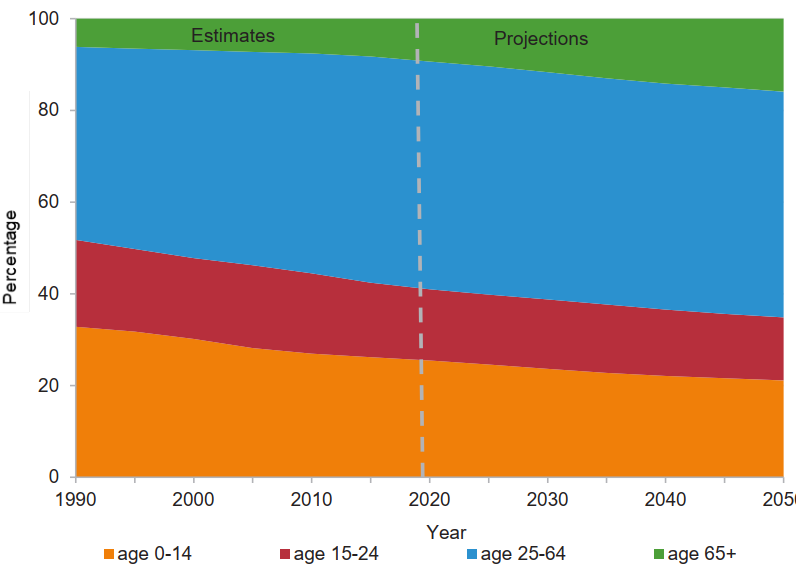
\includegraphics[width=0.75\textwidth]{bab2/ar_PopulationbyAge.png}
    \caption{Global population by age distribution.}
    \label{fig:PopulationbyAge}
\end{figure}

The global population of elderly individuals has been growing rapidly. This trend is predicted to continue growing significantly in the future. According to data from the United Nations (UN) in 2019, the global number of elderly people aged 65 years or older reached 703 million (9\% of the total global population). This number is projected to continue rising and double in the next three decades, which means 2050. Fig. \ref{fig:PopulationbyAge} illustrates the distribution of the global population categorized by age groups. The elderly population is expected to continue growing as the decline in the working-age population decreases.

% Populasi elderly di dunia telah meningkat secara pesat. Tren ini akan diprediksi terus bertambah banyak kedepannya. Berdasarkan data dari UN pada tahun 2019, jumlah elderly secara global telah mencapai jumlah 703 juta orang berusia 65 tahun atau lebih. Jumlah ini diproyeksikan akan terus meningkat dan menjadi dua kali lipatnya tiga dekade kedepan atau pada tahun 2050. Fig. \ref{fig:PopulationbyAge} menunjukkan pesebaran populasi global yang dibedakan berdasarkan rentang usia. Elderly diproteksikan akan terus bertambah seiring pengurangan penurunan masyarakat usia produktif.

As individuals age, they are highly likely to experience various physical and mental changes and conditions, such as decreased mobility, loss of sensory functions, depression, difficulty expressing themselves, and a decline in physical abilities. In some cases, the elderly require assistance in performing daily activities. Accompanying and providing support to the elderly has become a dedicated focus for researchers. Solving the issues related to the safety and daily care of the elderly requires research proposals in activity recognition \cite{elderly1}.

% Seiring bertambahnya usia, seseorang sangat mungkin mengalami kondisi dan perubahan pada dirinya baik secara fisik maupun mental, seperti penurunan mobilitas, hilangnya fungsi indera tubuh, depresi, kurangnya dalam mengekspresikan diri, hingga penurunan kemampuan fisik. Dalam beberapa kasus, elderly membutuhkan bantuan dalam menjalankan beberapa kegiatannya. Pendampingan terhadap elderly telah menjadi konsentrasi tersendiri bagi para peneliti. Penyelesaian masalah mengenai keamanan perawatan dan sehari-hari elderly membutuhkan usulan riset dalam pengenalan aktifitasnya \cite{elderly1}.

\section{Elderly Physical Issue}
\label{sec2:ElderlyPhysicalIssue}

The issue of eldelry health has become important since the increase in the number of elderly in the world. Increasing age makes the elderly experience a decrease in organ or tissue function. Diseases that affect the elderly can vary, such as chronic health problems, mobility and balance, decreased sensory function, and physical issues. For physical issues, diseases affect the muscles and bones of the elderly. Strengthening these body parts is important because they are the main support of the body \cite{PhysicalIssue}. Some of the physical issues that affect the elderly are explained in this section.

\subsection{Frozen Shoulder and Exercise Activity}
\label{subsec2:FrozenShoulder}

\begin{figure}[h!]
    \centering
    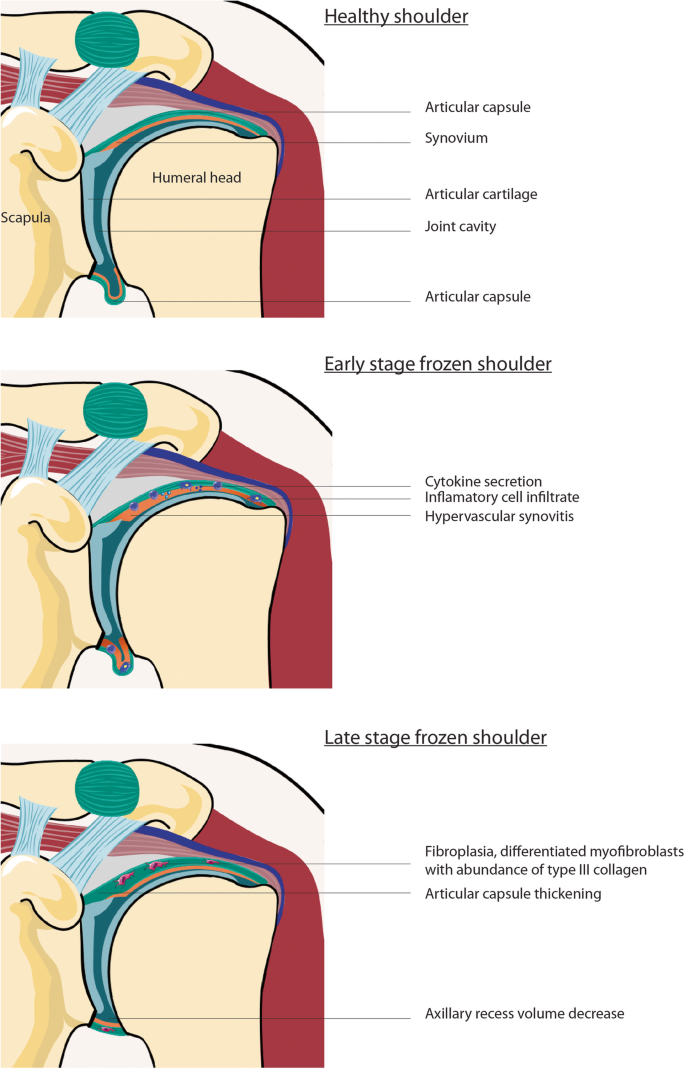
\includegraphics[width=0.75\textwidth]{bab2/ar_FrozenShoulder.png}
    \caption{Comparison of healthy shoulders with those with frozen shoulder \cite{FrozShoulder4}.}
    \label{fig:FrozenShoulder}
\end{figure}

Frozen shoulder, another name for adhesive capsulitis, is a common shoulder condition marked by a progressive rise in pain and stiffness. Women are more likely than males to be impacted, and it usually affects those over 40. The illness develops in three stages: freezing (painful), adhering, and melting. It usually goes away on its own in one to three years \cite{FrozenShoulder2}. There are two categories of frozen shoulder: primary and secondary. Primary frozen shoulder is caused by the presence of pericapsular attachments, while secondary frozen shoulder is caused by various factors such as sprains, strains, tendinopathy, tendon tears, or bursitis \cite{FrozenShoulder1}.

In the frozen period, strengthening activities such isometric shoulder external rotation, posterior capsule stretch, and scapular retraction might be introduced. Stretching and strengthening exercises can also get more intense during the thawing phase by holding onto the poses for longer periods of time.

Case studies demonstrate how well physical therapy works to improve joint mobility and day-to-day functioning. For instance, a case study published in the Journal of the Formosan Medical Association described how physiotherapy was used to treat a patient with primary frozen shoulder, leading to better joint mobility and ability to do everyday tasks.

These physical issues can be prevented using exercise activities. A wide variety of exercise activities can prevent these physical issues. Exercise activities that move the shoulder are the main focus of the movement. Some of the training activities are shoulder flexion extension \cite{ShoulderFlexionExtension}, adduction abduction \cite{AdductionAbduction}, and arm circumduction \cite{ArmCircumduction}.
% Isu fisik ini dapat dicegah menggunakan aktifitas latihan. Berbagai macam aktifitas latihan mampu mencegah munculnya isu fisik ini. Aktifitas latihan yang menggerakkan bagian bahu menjadi fokus utama pada gerakannya. Beberapa aktifitas latihan adalah shoulder flxion extension \cite{ShoulderFlexionExtension}, adduction abduction \cite{AdductionAbduction}, dan arm circumduction \cite{ArmCircumduction}.

Shoulder flexion and extension are the two main types of movements performed by the shoulder joint, which involve moving the arm around the body axis. Shoulder flexion is the movement of raising the arm forwards and upwards, away from the body. It involves muscles such as the anterior deltoid, pectoralis major and coracobrachialis. An example of this movement is when an individual lifts the arm straight forward until the arm is above the head. Shoulder extension is the movement of moving the arm behind the body. This movement involves muscles such as the posterior deltoid, latissimus dorsi, and teres major. An example of this movement is when individuals swing their arms backwards while walking or running \cite{ShoulderFlexionExtension1}.
% Shoulder flexion dan extension adalah dua jenis gerakan utama yang dilakukan oleh sendi bahu, yang melibatkan pergerakan lengan di sekitar sumbu tubuh. Shoulder flexion adalah gerakan mengangkat lengan ke depan dan ke atas, menjauh dari tubuh. Gerakan ini melibatkan otot-otot seperti deltoid anterior, pectoralis major, dan coracobrachialis. Contoh dari gerakan ini adalah ketika individu mengangkat lengan lurus ke depan hingga lengan berada di atas kepala. Shoulder extension adalah gerakan menggerakkan lengan ke belakang tubuh. Gerakan ini melibatkan otot-otot seperti deltoid posterior, latissimus dorsi, dan teres major. Contoh dari gerakan ini adalah ketika individu mengayunkan lengan ke belakang saat berjalan atau berlari \cite{ShoulderFlexionExtension1}.

Adduction and abduction arm movements are two types of movements that involve the displacement of the arm with respect to the body axis. Adduction is the movement of bringing the arm closer towards the centerline of the body. When the arm moves from a distant position towards the body is called adduction. For example, when an individual brings the arm to the side of the body. While abduction is the movement of moving the arm away from the midline of the body. When the arm moves from a position near the body outwards it is called abduction. For example, when individuals raise their arms to the side away from the body. These two movements in a series are often used in various physical activities and exercises to train certain muscles and increase flexibility and body strength \cite{AdductionAbduction1}.
% Gerakan lengan adduction dan abduction adalah dua jenis gerakan yang melibatkan perpindahan lengan terhadap sumbu tubuh. Adduction adalah gerakan mendekatkan lengan ke arah garis tengah tubuh. Ketika lengan bergerak dari posisi yang jauh ke arah tubuh disebut adduction. Sebagai contoh ketika individu merapatkan lengan ke sisi tubuh. Sedangkan abduction adalah gerakan menjauhkan lengan dari garis tengah tubuh. Ketika lengan bergerak dari posisi dekat tubuh ke arah luar disebut abduction. Sebagai contoh saat individu mengangkat lengan ke samping menjauh dari tubuh. Dua gerakan ini dalam satu rangkaian sering digunakan dalam berbagai aktivitas fisik dan latihan untuk melatih otot-otot tertentu dan meningkatkan fleksibilitas dan kekuatan tubuh \cite{AdductionAbduction1}.

Arm circumduction is a circular motion of the arm that incorporates several different shoulder joint movements, including flexion, extension, abduction, and adduction. During a circumduction movement, the arm moves in a cone shape, with the apex of the cone at the shoulder joint and the base of the cone at the hand. Circumduction is often seen in everyday activities such as throwing a ball or swimming freestyle. This movement allows the arm to move in multiple directions and achieve a variety of flexible positions, making it important for many sports and functional activities \cite{ArmCircumduction}.
% Gerakan arm circumduction adalah gerakan melingkar dari lengan yang menggabungkan beberapa gerakan sendi bahu yang berbeda, termasuk flexion, extension, abduction, dan adduction. Selama gerakan circumduction, lengan bergerak membentuk kerucut, dengan titik puncak kerucut berada di sendi bahu dan alas kerucut di tangan. Circumduction sering terlihat dalam aktivitas sehari-hari seperti melempar bola atau berenang gaya bebas. Gerakan ini memungkinkan lengan bergerak dalam berbagai arah dan mencapai berbagai posisi yang fleksibel, sehingga penting untuk banyak aktivitas olahraga dan fungsional \cite{ArmCircumduction}.

\subsection{Tennis Elbow and Exercise Activity}
\label{subsec2:TennisElbow}

\begin{figure}[h!]
    \centering
    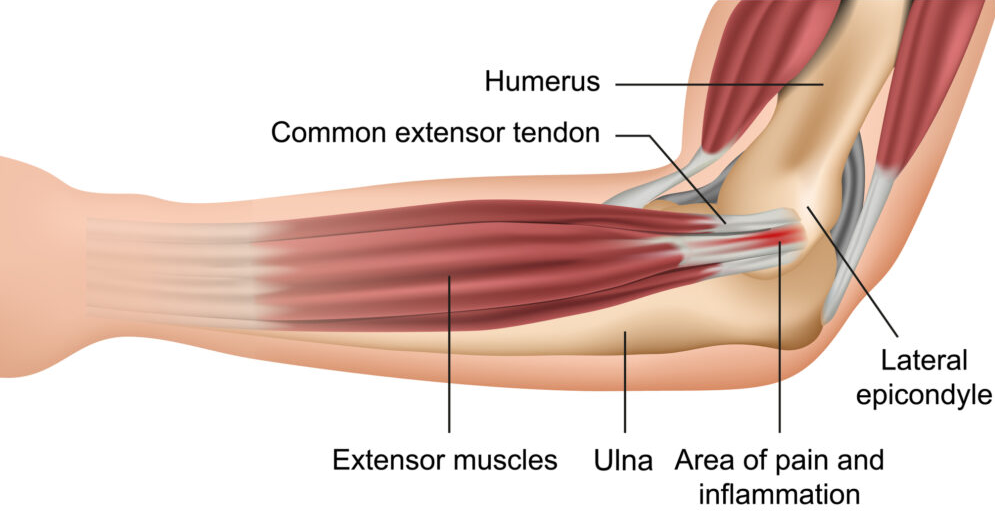
\includegraphics[width=0.8\textwidth]{bab2/ar_TennisElbow.png}
    \caption{Anatomy of tennis elbow. The area of pain and inflammation is shown in the region located around the lateral epicondyle, which is the main characteristic of this condition.}
    \label{fig:TennisElbow}
\end{figure}

Tennis elbow, often referred to as lateral epicondylitis, is a common musculoskeletal ailment marked by soreness and discomfort in the area of the elbow's common extensor origin. It is more prevalent in the dominant arm and is thought to impact 1\% to 3\% of adults annually. Though it can also happen as an acute injury (trauma to the lateral elbow), the condition is usually thought to be an overuse ailment requiring repetitive wrist extension against resistance \cite{TennisElbow1}.

Tennis elbow is characterized by pain and sensitivity in the area surrounding the lateral epicondyle, pain that gets worse as the middle finger and wrist are resisted, and elbow pain and stiffness. Repetitive forearm and hand motions, as those used in tennis, golf, and other sports, are frequently linked to the syndrome. People who perform repetitive gripping or lifting jobs at work may also experience it.

Case reports highlight the effectiveness of physiotherapy in improving joint movement and reducing pain. For example, a case series published in the Journal of Orthopaedic and Sports Physical Therapy detailed the use of dry needling as an alternative treatment for tennis elbow, resulting in significant improvements in patient-reported pain and function \cite{TennisElbow2}.

One of the training activities that can prevent the physical issue of tennis elbow is elbow flexion extension \cite{ElbowFlexionExtension}. The elbow flexion and extension movements are the two main types of movements performed by the elbow joint, which involve the movement of the forearm against the upper arm. Elbow flexion is the movement of bending the elbow so that the forearm comes closer to the upper arm. This movement involves muscles such as the biceps brachii, brachialis, and brachioradialis. Examples of this movement are when individuals bring their hands towards their shoulders or lift weights by bending their elbows. The elbow extension is the movement of straightening the elbow so that the forearm moves away from the upper arm. This movement involves muscles such as the triceps brachii and anconeus. Examples of this movement are when an individual pushes something away from the body or swings the arm into a straight position after bending it.
% Salah satu aktifitas latihan yang dapat mencegah terjadinya isu fisik tennis elbow adalah elbow flexion extension \cite{ElbowFlexionExtension}. Gerakan elbow flexion dan extension adalah dua jenis gerakan utama yang dilakukan oleh sendi siku, yang melibatkan pergerakan lengan bawah terhadap lengan atas. Elbow flexion adalah gerakan menekuk siku sehingga lengan bawah mendekat ke lengan atas. Gerakan ini melibatkan otot-otot seperti biceps brachii, brachialis, dan brachioradialis. Contoh dari gerakan ini adalah saat individu membawa tangan ke arah bahu atau mengangkat beban dengan menekuk siku. Adapun elbow extension adalah gerakan meluruskan siku sehingga lengan bawah menjauh dari lengan atas. Gerakan ini melibatkan otot-otot seperti triceps brachii dan anconeus. Contoh dari gerakan ini adalah saat seorang individu mendorong sesuatu menjauh dari tubuh atau mengayunkan lengan ke posisi lurus setelah menekuknya.

\subsection{Knee Pain and Exercise Activity}
\label{KneePain}
Knee pain is a common and multifaceted condition that can be caused by various factors, including osteoarthritis, patellofemoral pain, meniscal tears, and other conditions. About 25\% of adults exprience knee discomfort, a condition that has become much more common during the previous 20 years \cite{KneePain1}. Osteoarthritis, meniscal tears, patellofemoral discomfort, quadriceps or patellar tendinopathy, pes anserine bursitis, and iliotibial band syndrome are among the common causes. Running, crouching, and ascending stairs can all aggravate pain that is localized to particular parts of the knee, such as the anterior, medial, lateral, or posterior regions. A tool for determining the location and pattern of knee pain is the Knee Pain Map, which can be useful in both diagnosing and treating knee pain \cite{KneePain2, KneePain3}.

\begin{figure}[h!]
    \centering
    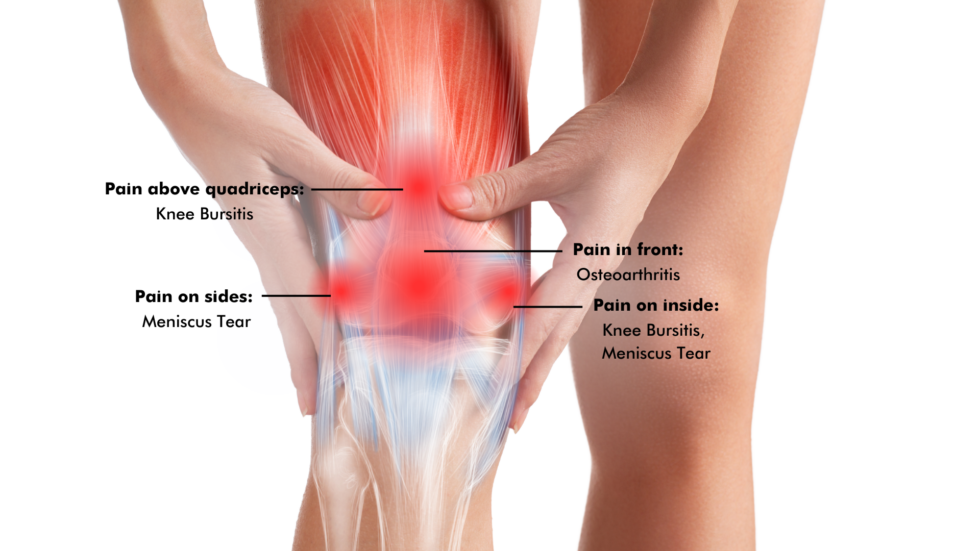
\includegraphics[width=0.9\textwidth]{bab2/ar_KneePain.png}
    \caption{Illustration of a set of issues located at the knee.}
    \label{fig:KneePain}
\end{figure}

There are two approaches in solving knee pain problems, namely exercise therapy and radiography. First-line management for osteoarthritis, patellofemoral pain, and meniscal tears often involves exercise therapy, weight loss (if overweight), education, and self-management programs to empower patients to better manage their condition \cite{KneePain4}. Radiography may be necessary to further evaluate undifferentiated knee pain, but should be reserved for chronic knee pain of more than six weeks duration or acute traumatic pain in patients who meet specific evidence-based criteria \cite{KneePain1}.

Knee pain is a frequent issue that has to be evaluated thoroughly. To confirm the diagnosis, a regular history and physical examination as well as imaging and laboratory tests may be necessary. Exercise therapy, weight loss, education, and self-management programs are common forms of treatment. In cases of severe meniscal tears or end-stage osteoarthritis, surgical referral is taken into consideration.

Exercise activities that can prevent this physical issue include leg flexion extension and knee flexion extension. Leg flexion and extension movements are the two main types of movements performed by the knee joint that involve the movement of the leg against the body. In the leg flexion stage, flexion of the knee is the movement of bending the knee so that the heel approaches the buttocks. The muscles involved in this movement include the hamstrings (biceps femoris, semitendinosus, and semimembranosus). Whereas in leg extension, extension of the knee is the movement of straightening the knee so that the leg returns to a straight position. The muscles involved include the quadriceps (rectus femoris, vastus lateralis, vastus medialis, and vastus intermedius). Leg bending and straightening movements are often performed in walking and running activities \cite{LegFlexionExtension}.
% Aktifitas-aktifitas latihan yang dapat mencegah terjadinya isu fisik ini diantaranya adalah leg flexion extension dan knee flexion extension. Gerakan leg flexion dan extension adalah dua jenis gerakan utama yang dilakukan oleh sendi lutut yang melibatkan pergerakan kaki terhadap tubuh. Pada tahap leg flexion, flexion pada lutut adalah gerakan menekuk lutut sehingga tumit mendekati bokong. Otot-otot yang terlibat dalam gerakan ini termasuk hamstrings (biceps femoris, semitendinosus, dan semimembranosus). Sedangkan pada leg extension, extension pada lutut adalah gerakan meluruskan lutut sehingga kaki kembali ke posisi lurus. Otot-otot yang terlibat termasuk quadriceps (rectus femoris, vastus lateralis, vastus medialis, dan vastus intermedius). Gerakan menekuk dan melurusan kaki sering dilakukan pada aktifitas berjalan dan berlari \cite{LegFlexionExtension}.

The knee flexion and extension movements are the two main types of movements performed by the knee joint, which involve the movement of the lower leg relative to the upper leg. In the knee flexion stage, the movement involves bending the knee so that the lower leg approaches the buttocks. The main muscles involved in this movement are the hamstrings, which consist of the biceps femoris, semitendinosus and semimembranosus. Movements that are often done daily such as squatting positions. As for knee extension, the movement that occurs is straightening the knee so that the lower leg moves away from the buttocks and returns to a straight position. The main muscles involved in this movement are the quadriceps, which consists of the rectus femoris, vastus lateralis, vastus medialis, and vastus intermedius. Daily activities that involve this movement include standing up from a squatting position \cite{KneeFlexionExtension}.
% Gerakan knee flexion dan extension adalah dua jenis gerakan utama yang dilakukan oleh sendi lutut, yang melibatkan pergerakan kaki bagian bawah terhadap kaki bagian atas. Pada tahap knee flexion, gerakan yang terjadi adalah menekuk lutut sehingga kaki bagian bawah mendekati bokong. Otot-otot utama yang terlibat dalam gerakan ini adalah hamstrings, yang terdiri dari biceps femoris, semitendinosus, dan semimembranosus. Gerakan yang sering dilakukan sehari-hari seperti posisi jongkok. Adapun knee extension, gerakan yang terjadi adalah meluruskan lutut sehingga kaki bagian bawah menjauh dari bokong dan kembali ke posisi lurus. Otot-otot utama yang terlibat dalam gerakan ini adalah quadriceps, yang terdiri dari rectus femoris, vastus lateralis, vastus medialis, dan vastus intermedius. Aktifitas sehari-hari yang melibatkan gerakan ini seperti berdiri dari posisi jongkok \cite{KneeFlexionExtension}.

\section{Human Pose Estimation}
Pose estimation is a field of computer vision research that has been widely developed for multiple purposes. Pose estimation involves detecting, associating, and tracking data points on body parts that represent the human body. Pose estimation focuses on estimating the positions of body parts using predefined keypoints. Pose estimation can also be used for tracking human activity. For instance, pose estimation from images or videos in motion is used for healthcare monitoring \cite{healthcare1,healthcare2}, sports \cite{sport1, sport2, sport3}, sign language understanding \cite{signlanguage1,signlanguage2,signlanguage3}, psychology \cite{Psychology1,Psychology2, Psychology3}, and human gesture control \cite{BlazePose, Heuristic}. Generally, human pose estimation consists of two approaches, i.e., the top-down approach and the bottom-up approach.


% Estimasi pose umumnya terdiri dari dua pendekatan, yaitu \textit{top-down} dan \textit{bottom-up}. Pendekatan \textit{top-down} dilakukan dalam dua tahap. Metode ini dimulai dengan pendeteksian orang, yang kemudian diikuti dengan penentuan pose mereka. Pendekatan ini membutuhkan komputasi yang banyak ketika jumlah orang yang terdeteksi dalam suatu \textit{frame} meningkat. High-Resolution Net (HRNet) \cite{HRNet} dan Mask R-CNN \cite{MaskRCNN} adalah beberapa model yang menggunakan pendekatan ini. Sebaliknya, pendekatan \textit{bottom-up} mendeteksi setiap sendi tubuh \textit{(keypoint)}, yang kemudian berkembang menjadi individu-tunggal. Metode ini memperkirakan probabilitas bahwa suatu sendi \textit{(keypoint)} tertentu akan hadir di piksel mana pun menggunakan peta probabilitas yang disebut \textit{heatmaps}. Pendekatan ini cukup sensitif terhadap jumlah orang dan resolusi gambar input. Berbagai penelitian terbaru telah meningkatkan pendekatan \textit{bottom-up}. Masalah pose manusia dalam resolusi gambar tertentu telah diusulkan dalam \cite{Openpose}.

\subsection{Top-Down Approach}
This method detects the persons first then the landmarks are localized for each person. The localization aims to determine the keypoints. An increase in the number of people indicates a higher level of computational complexity. They perform well on popular benchmarks in terms of accuracy. However, due to the complexity of these models, achieving real-time inference is computationally expensive \cite{YOLO-Pose}. The majority of top-down techniques now in use make use of human detector models like High-Resolution Net (HRNet) \cite{HRNet}, AlphaPose \cite{AlphaPose}, Feature Pyramid Networks \cite{Feature_Pyramid_Network}, Faster R-CNN \cite{FasterRCNN}, and Mask R-CNN \cite{MaskRCNN}. One of the first top-down models to use the Faster R-CNN for the person detection step is proposed by Papandreou et al. \cite{Papandreou}. The Cascaded Pyramid Network (CPN), developed by Chen et al. \cite{Cascade}, which integrates multi-scale feature maps from various GlobalNet layers with an online hard keypoint mining loss for challenging-to-detect joints.

\begin{figure}[h!]
    \centering
    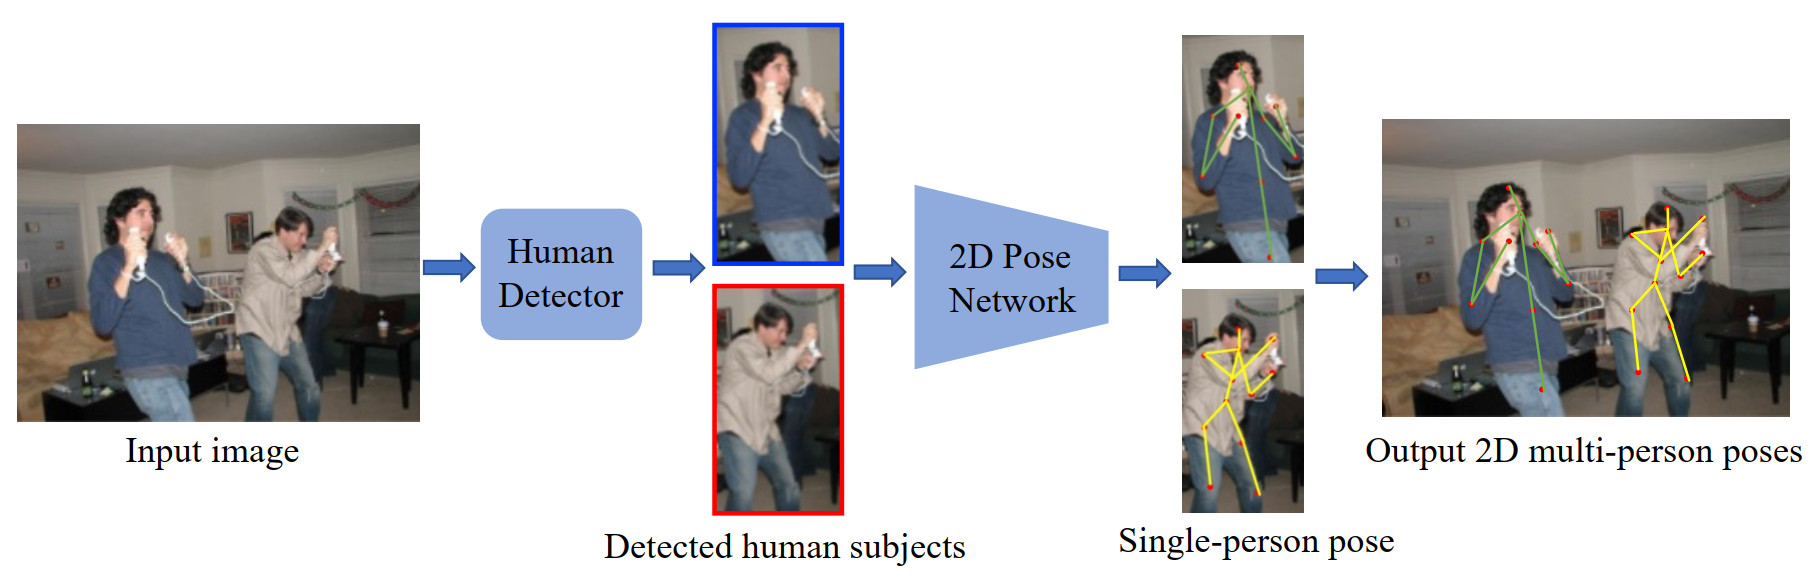
\includegraphics[width=0.9\textwidth]{bab2/ar_TopDown.png}
    \caption{Illustration of top-down approach in a 2D human pose estimation task \cite{HPEApproaches}.}
    \label{fig:TopDown}
\end{figure}

Figure \ref{fig:TopDown} shows an example of a top-down approach in human pose estimation. The process begins with an input image containing one or more people. The input image is then processed by a human detector that detects the presence of human subjects in the image. This human detector marks a bounding box around each detected individual. Once detected, the human subject is clearly identified within a bounding box. Then each individual in the image is processed in a separate state. One example of the model used is the 2D pose network. Each bounding box containing an individual is then fed into a 2D pose network. This network is responsible for estimating human poses so as to produce body keypoint coordinates for each detected subject. The resulting keypoints may vary depending on the deep learning model used. The result of this estimation is the pose of the individual in the form of keypoints connected by lines that indicate the basic skeletal of the body. After each individual has been estimated, the separate images are then reassembled according to the input image. This final image shows the pose estimation results together.
% Gambar \ref{fig:TopDown} menunjukkan contoh pendekatan top-down dalam estimasi pose manusia. Proses diawali dengan gambar input yang berisi satu atau lebih orang. Gambar input kemudian diproses oleh detektor manusia yang mendeteksi keberadaan subjek manusia dalam gambar. Detektor manusia ini menandai bounding box di sekitar setiap individu yang terdeteksi. Setelah terdeteksi, subjek manusia diidentifikasi dengan jelas dalam sebuah bounding box. Kemudian setiap individu dalam gambar diproses dalam kondisi terpisah. Salah satu contoh model yang digunakan adalah 2D pose network. Setiap bounding box yang berisikan individu ini kemudian dimasukkan ke dalam 2D pose network. Jaringan inilah yang bertanggung jawab dalam mengestimasi pose manusia sehingga menghasilkan koordinat keypoint tubuh untuk setiap subjek yang terdeteksi. Keypoint yang dihasilkan dapat berbeda-beda, bergantung pada model deep learning yang digunakan. Hasil dari estimasi ini adalah pose individu dalam bentuk keypoint yang terhubung oleh garis-garis yang menunjukkan skeletal dasar dari tubuh. Setelah setiap individu terestimasi, setiap gambar yang terpisah tadi kemudian disatukan kembali sesuai dengan gambar input. Gambar akhir ini menunjukkan hasil estimasi pose secara bersamaan.

\subsection{Bottom-Up Approach}
In this approach, it finds keypoints of all the persons in an image at once, followed by grouping them into individual persons \cite{bottom-up}. A probabilistic map called heatmap is used by these approaches to estimate the probability of every pixel containing a particular landmark (keypoint). With the help of Non-Maximum Suppression, the best landmark is filtered. These are less complex compared to Top-down methods but at the cost of reduced accuracy \cite{YOLO-Pose}. The method adopted to group recognized body parts in a picture is where different techniques diverge. Some examples of these approach models are OpenPose \cite{Openpose}, PifPaf \cite{PifPaf}, and single-stage encoder-decoder \cite{Nimbro}. To forecast keypoint heatmaps and part affinity fields, which are 2D vectors describing the relationships between joints, OpenPose \cite{Openpose} creates a model with two branches. In the grouping procedure, an affinity field is employed in part. Using the embedding spaces, Pose Partition Networks \cite{PosePartitionNetwork} propose a dense regression method across all the keypoints to construct individual partitions.

\begin{figure}[h!]
    \centering
    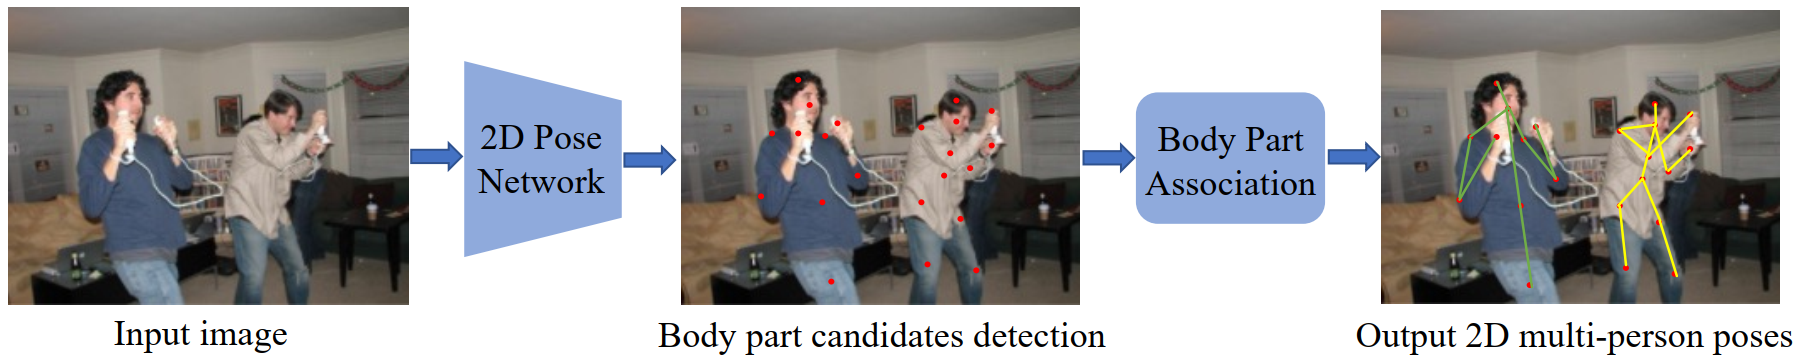
\includegraphics[width=0.9\textwidth]{bab2/ar_BottomUp.png}
    \caption{Illustration of top-down approach in a 2D human pose estimation task \cite{HPEApproaches}.}
    \label{fig:BottomUp}
\end{figure}

Figure \ref{fig:BottomUp} shows an example of a bottom-up approach in human pose estimation. For example, the model used in this estimation is a 2D pose network. The process starts with an input image containing single or multiple individuals. This input image is processed by the 2D pose network. This network is responsible for detecting possible humans in the input image. In the detection process, the network will first detect human body candidates. These points indicate the possible locations of certain body parts depending on the keypoints specified by the model. The next process is human body association. Each of these points will be connected to each other to form the skeleton of a human pose. This process matches the detected body parts into the human skeletal structure of each person in the image. The end of this approach is a multi-person pose. The result is the complete pose of each person in the image, displayed with keypoints connected by lines indicating the skeletal structure.
% Gambar \ref{fig:BottomUp} menunjukkan contoh pendekatan bottom-up dalam estimasi pose manusia. Sebagai contoh, model yang digunakan pada estimasi ini adalah 2D pose network. Proses diawali dengan sebuah gambar input yang berisikan dengan individu tunggal maupun multi. Gambar input ini diproses oleh 2D pose network. Jaringan inilah yang bertanggun jawab dalam mendeteksi kemungkinan-kemungkinan manusia yang berada di dalam gambar input. Dalam proses deteksinya, jaringan akan mendeteksi kandidat-kandidat tubuh manusia terlebih dahulu. Titik-titik ini menunjukkan kemungkinan lokasi bagian tubuh tertentu bergantung pada keypoint yang ditentukan oleh model. Proses berikutnya adalah asosiasi tubuh manusia. Setiap titik-titik ini akan dihubungkan satu sama lain membentuk kerangka pose manusia. Proses ini mencocokkan bagian tubuh yang terdeteksi ke dalam struktur kerangka manusia setiap orangnya dalam gambar. Akhir dari pendekatan ini adalah pose untul multi-orang. Hasilnya adalah pose lengkap dari setiap orang dalam gambar, ditampilkan dengan keypoint yang terhubung oleh garis yang menunjukkan struktur skeletal.

\section{MediaPipe Pose Estimation}
One of the frameworks for human pose estimation is Mediapipe Pose Estimation (MPE). MPE is an open-source cross-platform framework provided by Google for estimating 2D human joint coordinates in each image frame \cite{MPE}. MPE builds pipelines that analyzes cognitive data provided as video using machine learning (ML).

\begin{figure}[H]
    \centering
    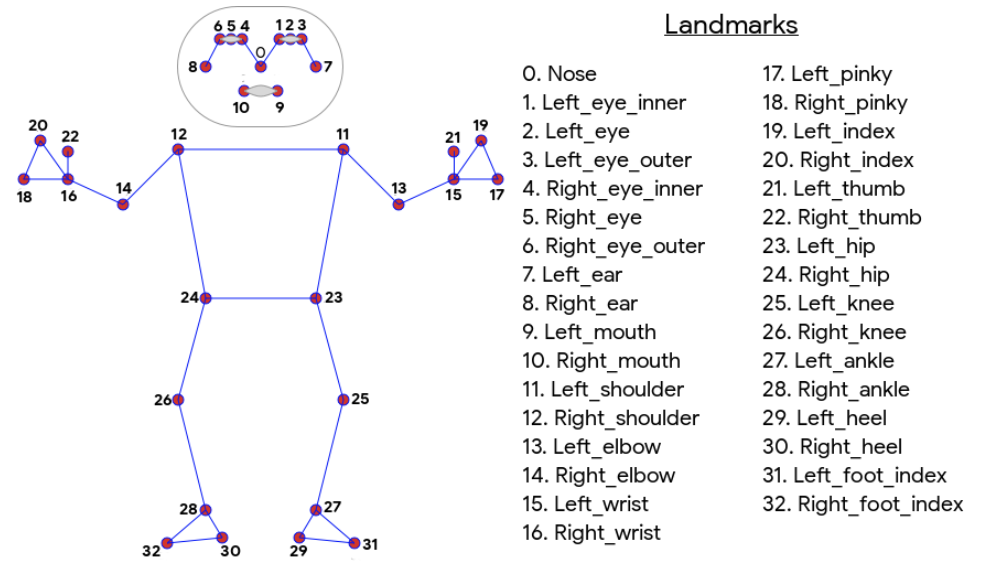
\includegraphics[width=1\textwidth]{bab2/ar_BlazePoseKeypointTopology.png}
    \caption{BlazePose keypoint topology.}
    \label{fig:BlazePoseKeypointTopology}
\end{figure}

The backbone architecture behind this framework is called BlazePose \cite{BlazePose}. Fig.\ref{fig:InferencePipeline} shows the inference workflow of BlazePose architecture. The pose estimate component of BlazePose architecture predicts the location of all 33 person keypoints. During inference, the architecture adopt a detector-tracker configuration, which displays good real-time performance on a range of applications such as hand landmark prediction \cite{MediaPipeHands} and dense face landmark prediction \cite{MediaPipeDenseFace}. This pipeline comprises of a lightweight body pose detector followed by a pose tracker network. The tracker predicts keypoint coordinates, the presence of the person on the current frame, and the refined region of interest for the current frame. When the tracker reports that there is no human present, the architecture re-run the detection network on the following frame.

Pose estimation using the BlazePose architecture offers the advantage of producing lightweight models. For low-computational devices, a lightweight model is highly preferred. BlazePose is a lightweight convolutional architecture designed for real-time pose estimation. On a single mid-tier phone CPU, the frame rate for the BlazePose Full architecture is 10 FPS while the BlazePose Lite architecture is 31 FPS \cite{BlazeFace}.

\begin{figure}[h!]
    \centering
    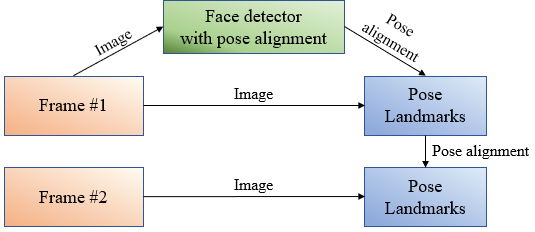
\includegraphics[width=0.75\textwidth]{bab2/ar_InferencePipeline.png}
    \caption{Inference workflow of BlazePose architecture \cite{BlazePose}.}
    \label{fig:InferencePipeline}
\end{figure}

\section{Deep Learning}
\label{sec2:DeepLearning}

Deep learning is a branch of machine learning that uses artificial neural networks to analyze and extract patterns from large and complex data. Artificial neural networks, which are composed of linked layers of artificial neurons, including input layers, hidden layers, and output layers, are computer models that are modeled after the structure and operation of the human brain. The utilization of numerous hidden layers, which enables the model to learn increasingly complicated data representations, is one of the primary features of deep learning \cite{DL3}.

Deep learning is particularly effective when used on large and diverse datasets, allowing the model to improve accuracy and performance. The learning process in deep learning involves optimizing model parameters using algorithms such as stochastic gradient descent (SGD) and backpropagation techniques to update the weights in the neural network based on the error gradient, allowing the network to learn from errors.

\begin{figure}[H]
    \centering
    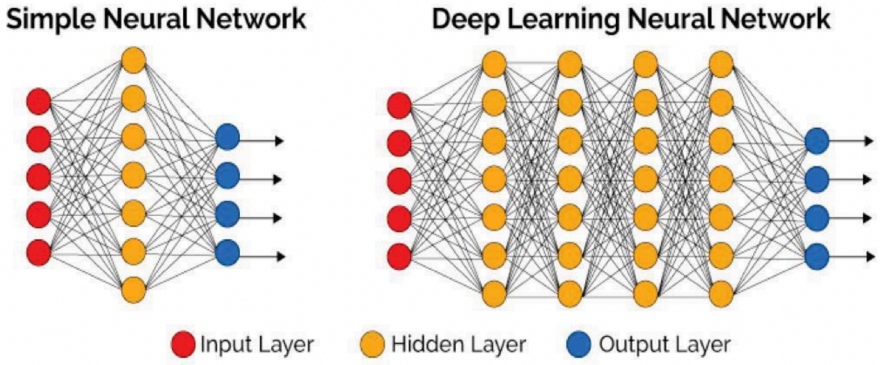
\includegraphics[width=0.9\textwidth]{bab2/ar_DLArchitecture.png}
    \caption{Compared between simple neural network architecture and deep learning neural network.}
    \label{fig:DLArchitecture}
\end{figure}

Deep Learning is a type of machine learning that excels in working with unstructured data. It has the capability to process a huge number of characteristics \cite{DL1}. Deep Learning algorithms process data over numerous levels. Each layer in Deep Learning increasingly extracts features and transmits them to the next layer. The early layers in Deep Learning are responsible for extracting low-level information, while subsequent layers combine various features to build a full representation. Deep Learning is connected to artificial neural networks, which are algorithms based on the structure and function of the brain.

Deep Learning enables computational models with several layers of processing to learn various degrees of abstraction for data representation. The layers in Deep Learning are neural networks with more than three layers of neurons (including input and output layers). More layers and neurons can represent increasingly complicated models, but they also require more time and resources for processing. The depiction of the Deep Learning architecture is presented in Figure \ref{fig:DLArchitecture} \cite{DL2}.

Types of deep learning networks include Convolutional Neural Networks (CNN) used in image and video processing, Recurrent Neural Networks (RNN) suitable for sequential data such as text and audio, and Generative Adversarial Networks (GAN) used for data generation. Applications of deep learning include image and speech recognition, natural language processing (NLP), autonomous vehicles, medical data analysis, and recommendation systems.

Deep learning has revolutionized many fields with the ability to learn and generalize from complex and unstructured data, enabling the development of advanced technologies such as virtual assistants and automated medical diagnosis.

\subsection{Convolutional Neural Network (CNN)}
CNN (Convolutional Neural Network) has applications in image and video recognition, recommendation systems, image classification, medical image analysis, natural language processing, and financial time series analysis. Traditional neural network methods do not perform well when it comes to image processing and need breaking down pictures into low-resolution patches. CNN has neurons arranged as portions involved for processing visual input in humans and other. The layers of neurons are designed in such a manner that they span the full visual field to avoid the gradual image processing difficulties of typical neural networks. The sequence of CNN layers includes of input layers, output layers, and hidden layers that contain numerous convolutional layers, pooling layers, and fully connected layers, as depicted in Figure \ref{fig:CNNArchitecture} \cite{CNN1}.

\begin{figure}[H]
    \centering
    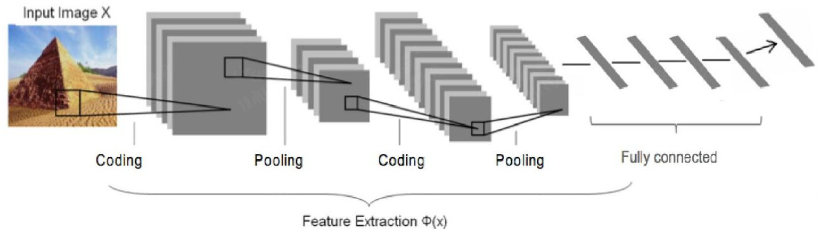
\includegraphics[width=1\textwidth]{bab2/ar_CNNArchitecture.png}
    \caption{An example of CNN architecture for image recognition \cite{cnnarch}.}
    \label{fig:CNNArchitecture}
\end{figure}

Convolution operation is a crucial component of convolutional neural networks. The convolutional layer consists of parameters that comprise a set of learnable filters (kernels). Each filter in this layer is small in width and height but extends through the full depth of the input volume. The commonly used filter sizes are 3x3, 5x5, and 7x7. The third dimension of the filter corresponds to the number of channels in the input. The depth of a grayscale image is 1, while a color image has 3 color channels (RGB).

CNN often employs pooling layers after the convolutional layers. These layers serve to lower the dimensions, often known as subsampling or downsampling. The hyperparameters of the pooling layer are the filter size and stride. The most typically used pooling layer has a filter size of 2 and a stride of 2. There are two main forms of pooling: max pooling, which takes the maximum value, and average pooling, which takes the average value. Max pooling is more often utilized than average pooling.

After several convolutional and pooling layers, CNN typically ends with several fully connected layers. The tensors from the output of these layers are flattened into vectors and then passed through several neural network layers. The dropout regularization technique can be applied to the fully connected layers to prevent overfitting. The final fully connected layer in the architecture contains the same number of output neurons as the number of classes to be recognized in an object detection model.

\subsection{Long Short-Term Memory (LSTM)}
LSTM network is an enhanced special network architecture of Recurrent Neural Network (RNN) \cite{RNN} which has its major usage in evaluating time series data of many disciplines. LSTM was meant to reduce the drawbacks of RNN such as vanishing gradient because of having short term memory. LSTM is capable of modeling the time series sequential data. A memory unit known as the cell was introduced in the network. As a result, LSTM can overcome the long-range dependency issue of RNN as it can keep the findings for a long-range of time \cite{LSTM1}.

\begin{figure}[H]
    \centering
    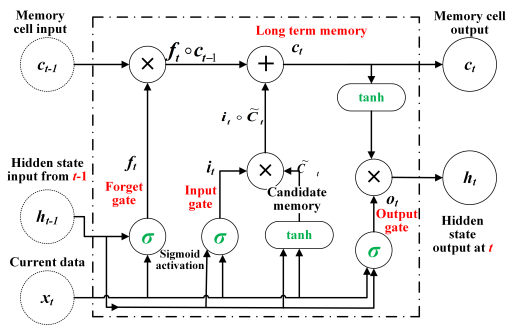
\includegraphics[width=0.75\textwidth]{bab2/ar_OneCellLSTM.png}
    \caption{Illustration of one cell of the LSTM memory block.}
    \label{fig:OneCellLSTM}
\end{figure}

The fundamental LSTM unit is shown in Fig. \ref{fig:OneCellLSTM}, and is made of a cell with an input gate, output gate, and forget gate. LSTMs use the concept of gating to deal with the disappearing or exploding gradient problem \cite{LSTM2}. The cell is responsible for remembering values over arbitrary time intervals, and each of the three gates can be thought of as a conventional artificial neuron, computing an activation (using an activation function) of a weighted sum of the current data $x_{t}$, a hidden state $h_{t-1}$ from the previous time step, and any bias $b$. Intuitively, the gates can be considered as regulators of the flow of values through the connections of the LSTM. At each time step they govern which action is done by the cell as stated below. In \ref{equ:WriteOperation} through \ref{equ:Output}, $w_{i}$ are the weights associated with each multiplication at gate $i$, while $\sigma$ and $tanh$ are possibilities for the activation functions.

Based on Fig. \ref{fig:OneCellLSTM}, the output gate controls the amount to which a new value flows into the cell, known as a write operation:
\begin{equation}
    \label{equ:WriteOperation}
    i_t=\sigma(w_i[h_{t-1},x_t]+b_i)
\end{equation}

The forget gate performs a similar process, regulating the amount to which the current cell value is preserved, executing a reset operation
\begin{equation}
    \label{equ:ResetOperation}
    f_t=\sigma(w_f[h_{t-1},x_t]+b_f)
\end{equation}

The candidate memory cell is updated similarly as:
\begin{equation}
    \label{equ:NewCandidateValue}
    \tilde{C}_t=\tanh(w_c[h_{t-1},x_t]+b_c)
\end{equation}

and by merging these distinct internal values the internal long-term memory or the next cell memory is formed as
\begin{equation}
    \label{equ:Combination}
    c_t=f_t*c_t+i_t*\tilde{C}_t
\end{equation}

From this, the cell output is created by the output gate to regulate the extent to which the value in the cell is utilized to compute the output activation, conducting a read operation:
\begin{equation}
    \label{equ:ReadOperation}
    o_t=\sigma(w_o[h_{t-1},x_t]+b_o)
\end{equation}

Lasltly, the cell's hidden output is found as
\begin{equation}
    \label{equ:Output}
    h_t=o_t*\tanh(c_t)
\end{equation}

\section{Performance Metrics}
\label{sec3: performance_metrics}

Performance metrics in deep learning are measures used to evaluate model performance. They offer information on how well the model can forecast new and never-before-seen data. Large datasets are frequently used to train models in deep learning, and performance metrics are used to evaluate the model's performance under various conditions. Here are some commonly used performance metrics in deep learning.

\subsection{Confusion Matrix}
\label{subsec3: confusion_matrix}
The confusion matrix is a tool used to measure the performance of a classification model by providing a detailed overview of the model's predictions against the test data. It is a box-shaped matrix that shows the number of correct and incorrect predictions made by the model. The number of predictions is based on the actual class and the predicted class. Figure A shows the elements in the confusion matrix, namely True Positive (TP), True Negative (TN), False Positive (FP), and False Negative (FP). Through this matrix, various performance metrics can be measured, such as precision, recall, accuracy, and loss.
% Confusion matrix adalah alat yang digunakan untuk mengukur kinerja model klasifikasi dengan memberikan gambaran rinci tentang hasil prediksi model terhadap data uji. Matriks ini berbentuk kotak yang memperlihatkan jumlah prediksi benar dan salah yang dibuat oleh model. Jumlah prediksi tersebut didasarkan kepada kelas yang sebenarnya dengan kelas yang diprediksi. Gambar A menunjukkan elemen-elemen di dalam confusion matrix, yaitu True Positive (TP), True Negative (TN), False Positive (FP), dan False Negative (FP). Melalui matrix ini, berbagai peforma metric dapat diukur, seperti  presisi, recall, akurasi, dan loss.

\begin{figure}[h!]
    \centering
    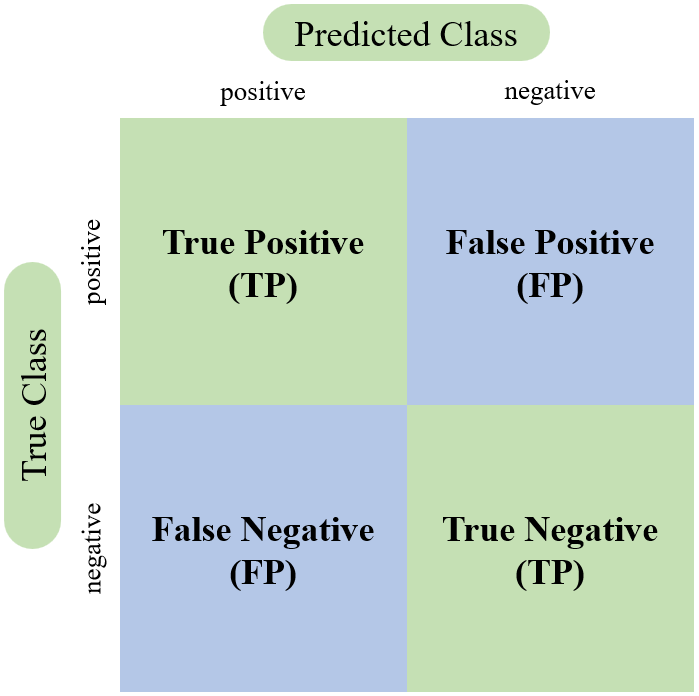
\includegraphics[width=0.5\textwidth]{bab2/ar_confmatrix.png}
    \caption{A common example of a confusion matrix.}
    \label{fig: convmatrix}
\end{figure}

\subsection{Accuracy}
\label{subsec3: accuracy}

\begin{figure}[h!]
    \centering
    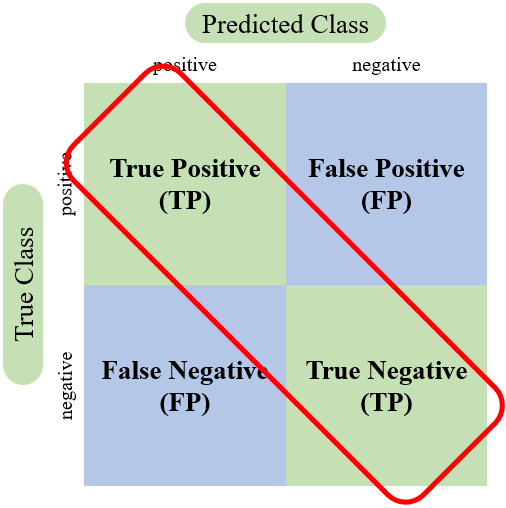
\includegraphics[width=0.5\textwidth]{bab2/ar_Accuracy.png}
    \caption{Accuracy is calculated as the ratio of the number of correct predictions to the total number of predictions.}
    \label{fig:MetricAccuracy}
\end{figure}

Accuracy is an evaluation measure used to assess model performance by calculating the proportion of correct predictions to total predictions. Accuracy shows how well the model performs overall. The accuracy equation is directly proportional to the True Positive (TP) and inversely proportional to the total prediction samples as shown in equation \ref{equ:accuracy}.
% Akurasi merupakan ukuran evaluasi yang digunakan untuk menilai kinerja model dengan menghitung proporsi prediksi yang benar terhadap total prediksi keseluruhan. Akurasi menunjukkan seberapa baik peforma model secara keseluruhan. Persamaan akurasi berbanding lurus dengan True Positive (TP) dan berbanding terbalik dengan total sampel prediksi sebagaimana ditunjukkan pada persamaan \ref{equ:accuracy}.

\begin{equation}
    \label{equ:accuracy}
    accuracy=\frac{TP+TN}{TP+TN+FP+FN}
\end{equation}

\subsection{Loss}
\label{equ:loss}
Loss is a function used to calculate the error of the deep learning model during the learning process. It is a quantitative measure that describes how well or poorly the model predicts the class of the input data compared to the ground truth. This function gives an indication of how far the model's prediction is from the correct value with the aim of minimizing the loss value during the training process to improve the accuracy and overall performance of the model.
% Loss merupakan fungsi yang digunakan untuk menghitung kesalahan model deep learning selama proses learning. Metris ini adalah ukuran kuantitatif yang menggambarkan seberapa baik maupun buruk model dalam memprediksi kelas dari data input dibandingkan dengan groun truth. Fungsi ini memberikan indikasi seberapa jauh prediksi model dari nilai yang benar dengan tujuan meminimalkan nilai loss selama proses pelatihan untuk meningkatkan akurasi dan kinerja model secara keseluruhan.

\subsection{Precision}
\label{subsec3: precision}

\begin{figure}[h!]
    \centering
    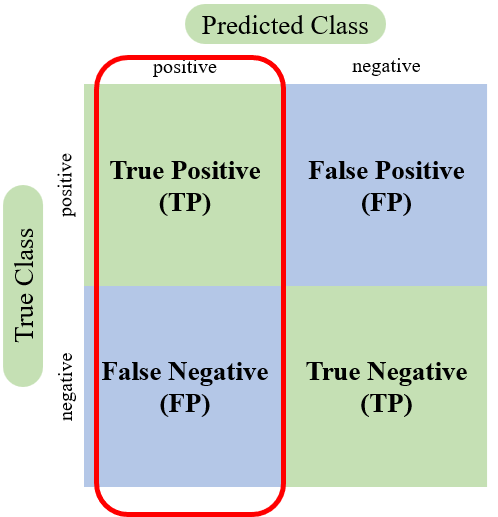
\includegraphics[width=0.5\textwidth]{bab2/ar_Precision.png}
    \caption{Precision is calculated as the ratio of the number of correct positive predictions to the total number of positive predictions made by the model.}
    \label{fig:MetricPrecision}
\end{figure}

Precision is a metrics that measures the proportion of correct positive predictions out of all predictions. Precision measures how well the model can find True Positive (TP) out of all positive predictions (TP+FP). The higher the precision value, the more positive predictions are predicted to be true. This metric becomes very important when in a situation where the false positive value is high. Precision is formulated in the equation \ref{equ:precision}.
% Precision adalah metrics yang mengukur proporsi prediksi positif yang benar dari semua prediksi. Precision mengukur seberapa baik model dapat menemukan True Positive (TP) dari semua prediksi positif (TP+FP). Semakin tinggi nilai precision menunjukkan semakin banyak prediksi positif yang diprediksi benar. Metric ini menjadi sangat penting ketika berada dalam situasi di mana nilai false positive tinggi. Precision dirumuskan pada persamaan \ref{equ:precision}. 

\begin{equation}
    \label{equ:precision}
    precision=\frac{TP}{TP+FP}
\end{equation}

\subsection{Recall}
\label{subsec3: recall}

\begin{figure}[h!]
    \centering
    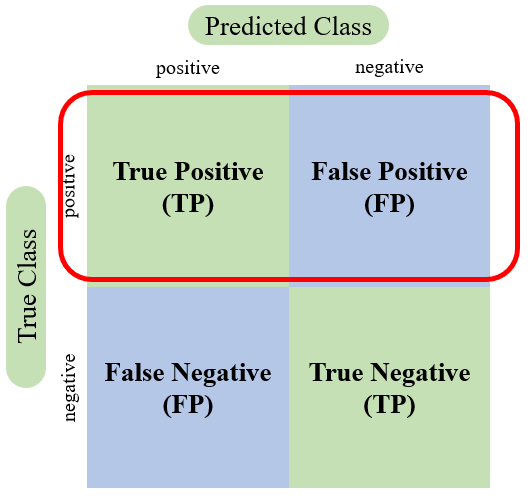
\includegraphics[width=0.5\textwidth]{bab2/ar_Recall.png}
    \caption{Recall is calculated as the ratio of the number of correct positive predictions to the total number of positive examples actually present in the dataset.}
    \label{fig:MetricRecall}
\end{figure}

This metric is used to measure how well the model can detect all positive events among all events that are actually positive. This metric becomes very important when false negatives have a significant probability. Recall is calculated as True Positive (TP) divided by the sum of True Positive and False Negative (TP+FN), according to the equation \ref{equ:recall}.
% Metric ini digunakan untuk mengukur seberapa baik model dapat mendeteksi seluruh kejadian positif di antara seluruh kejadian yang sebenarnya positif. Metric ini menjadi sangat penting ketika false negative memiliki kemungkinan yang signifikan. Recall dihitung sebagai True Positive (TP) dibagi dengan jumlah True Positive dan False Negative (TP+FN), sesuai dengan persamaan \ref{equ:recall}.

\begin{equation}
    \label{equ:recall}
    recall=\frac{TP}{TP+FN}
\end{equation}

\subsection{F1-Score}
\label{subsec3: f1score}
Another metric used is F1 score. The F1 score is a metric commonly used to measure the performance of a classification model. It is the harmonic mean of precision and recall. The F1 score combines precision and recall into a single value, providing a balanced measure of the model's performance. It is calculated using the following equation \ref{equ:f1score}.

\begin{equation}
    \label{equ:f1score}
    F1 score = 2 * \frac{precision * recall}{precision + recall}
\end{equation}

	\cleardoublepage
	\chapter{METHODOLOGY}
\label{sec:chap3_metodologi}

\section*{ }
This section describes our proposed method for pose estimation-based classification of elderly exercise activities using deep learning. We begin our work by determining the types of exercises that the elderly can do to address health issues in old age. One of the challenges of our work is the limited dataset available. So in collecting datasets, we created new datasets according to the predetermined dataset classes. The dataset we have is then subjected to preprocessing and keypoint extraction. The keypoint extraction set is trained using deep learning architecture to produce the desired model. The results of this model are then subjected to evaluation metrics to review our model. Figure \ref{fig:blokdiagram} provides a brief summary of the proposed method.

\begin{figure}[h!]
	\centering
	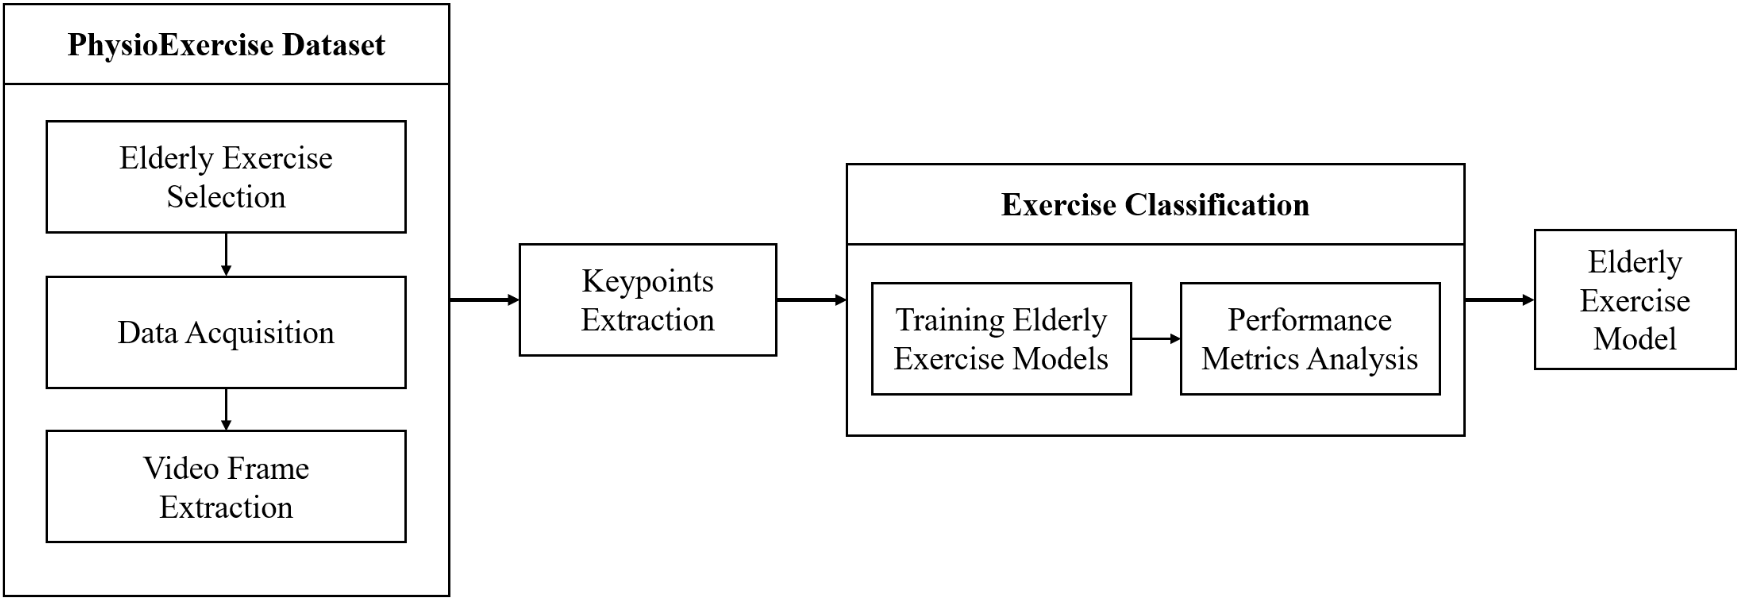
\includegraphics[width=\linewidth]{bab3/ar_BlockDiagram4.png}
	\caption{Research Block Diagram}
	\label{fig:blokdiagram}
\end{figure}

\section{PhysioExercise Dataset}
\label{sec3:physioexercise_dataset}
Exercise performed by the elderly is different from exercise performed in general. Since the elderly have special issues regarding their health, the exercises given must be adapted to their conditions. There are not many exercise datasets for the elderly. Therefore, this section explains the process of creating a dataset that is suitable for elderly exercise activities.
% Exercise yang dilakukan oleh elderly berbeda dengan exercise yang dilakukan secara umum. Sejak elderly memiliki isu-isu khusus mengenai kesehatannya, exercise yang diberikan harus disesuaikan dengan kondisi mereka. Tidak banyak dataset exercise untuk elderly. Oleh karena itu, bagian ini menjelaskan proses pembuatan dataset yang sesuai untuk aktifitas exercise elderly.


\subsection{Elderly Exercise Selection}
\label{subsec3:elderly_exercise_selection}
As a first step in our work, we had to determine the types of exercises for the elderly. Most human activity recognition, especially for the elderly, revolves around daily activities such as standing, sitting, lying down, eating, opening doors, etc. \cite{elderly2, elderly1}. Exercises performed for the elderly must be more selective and careful due to their physical condition. Therefore, it must be consulted with physiotheraphists first. In addition, the exercises that will be categorized are the types of exercises that can be done alone and at home. One example of exercises that fit the criteria is in \cite{dataset1}. The work shows physiotherapy activities for the elderly that can be done at home. In addition, the exercises are specialized based on health issues that are common to the elderly physique.

\subsection{Dataset Acquisition}
\label{subsec3:dataset_acquisition}
We made adjustments to the dataset we used. The dataset used is a collection of physiotherapy exercise videos for the elderly based on predetermined classes. The videos were taken in our laboratory and some were taken in the home environment. Since the utilization of physiotherapy exercises is done at home independently, the use of mobile phone cameras is one of the effective solutions. Therefore, we used mobile phone cameras as input for dataset capture. The camera specifications used in this work are 64 MP, 26mm focal length, f/1.8 aperture lens, 0.8µm pixel size, and 1/1.7" sensor size. The dataset was captured in the form of a 1080p resolution video. There is 30 frames per second in the video.

We varied the angle of the video capture. We placed the camera at 3 angles, i.e., straight ahead, \ang{30} angle relative to the left, and \ang{30} angle relative to the right. In addition to the camera angle, we also gave people a variety of angles. We apply various orientations of the person's position to the camera. This aims to enrich our dataset. However, we limit these orientations to the possible positions of the elderly in performing physiotherapy exercises.

\subsection{Video Frame Extraction}
\label{subsec3:VideoExtraction}

The acquired data is a collection of exercise activity videos. This data is organized in each folder according to the predefined class classification. We perform data preprocessing after we have collected all the required video datasets. We divided each video into 100 images. These images are sequences of physiotherapy exercise activities for each class that will have their keypoint values extracted. We have selected the videos so that they still have a high diversity value for each class.
% Data yang telah diakuisisi merupakan kumpulan video aktifitas latihan. Data ini diorganisir dalam masing-masing folder sesuai dengan klasifikasi kelas yang telah ditentukan sebelumnya. Kami melakukan prapemrosesan data setelah kami mengumpulkan semua set data video yang diperlukan. Kami membagi setiap video menjadi 100 gambar. Gambar-gambar ini adalah urutan kegiatan latihan fisioterapi untuk setiap kelas yang akan diekstraksi nilai keypoint-nya. Kami telah memilih video-video tersebut sehingga masih memiliki nilai keragaman yang tinggi untuk setiap kelas.

\section{Keypoint Extraction}
\label{sec:keypoint_extraction}

In this stage, we focus on the keypoint feature extraction process which is crucial for human motion analysis in the context of exercise activity classification for the elderly. This keypoint extraction is performed by utilizing the MediaPipe framework, a solution developed by Google to enable real-time and accurate human pose estimation. MediaPipe facilitates the extraction of keypoint coordinates by using machine learning models that have been trained on large and diverse datasets, enabling efficient human body position detection.
% Dalam tahap ini, kami fokus pada proses ekstraksi fitur keypoint yang krusial untuk analisis gerak manusia dalam konteks klasifikasi aktivitas latihan untuk elderly. Ekstraksi keypoint ini dilakukan dengan memanfaatkan framework MediaPipe, sebuah solusi yang dikembangkan oleh Google untuk memungkinkan estimasi pose manusia secara real-time dan akurat \cite{BlazePose}. MediaPipe memfasilitasi ekstraksi koordinat keypoint dengan menggunakan model pembelajaran mesin yang telah terlatih pada dataset yang luas dan beragam, memungkinkan deteksi posisi tubuh manusia secara efisien.

The extraction process begins with the receipt of video frames as input, where each frame first undergoes pre-processing to ensure that the incoming data is in optimal condition for analysis. Normalization is performed on the obtained pixel coordinates, converting them to a scale that is consistent and independent of the original dimensions of the image, thus enabling accurate comparisons among different sources and image resolutions. Coordinate normalization is done following equations \eqref{eq: pers.1} and \eqref{eq: pers.2}.
% Proses ekstraksi dimulai dengan penerimaan frame video sebagai input, di mana setiap frame pertama-tama mengalami pra-pemrosesan untuk memastikan bahwa data yang masuk dalam kondisi optimal untuk analisis. Normalisasi dilakukan pada koordinat piksel yang diperoleh, mengkonversi mereka ke skala yang konsisten dan independen dari dimensi asli gambar, sehingga memungkinkan komparasi yang akurat di antara berbagai sumber dan resolusi gambar.

\begin{equation}\label{eq: pers.1}
	(x',y') = \left(\frac{x}{widht},\frac{y}{height}\right)
\end{equation}

Width and height refer to image dimensions. Equation \eqref{eq: pers.2} refers to depth normalization (z-depth). The minimun and maximum depths represented by \(z\textsubscript{min}\) and \(z\textsubscript{max}\) are detected within the frame or a preset range.

\begin{equation}\label{eq: pers.2}
	z' = \frac{z-z_{min}}{z_{max}-z_{min}}
\end{equation}

After preprocessing, the frames are processed using MediaPipe's pose estimation model that uses a Convolutional Neural Network (CNN) architecture. This model effectively identifies and tracks 33 keypoints located in key areas of the human body, such as the head, shoulders, elbows, wrists, hips, knees and ankles. Each keypoint is detected with \((x, y, z)\) coordinates and comes with a confidence score that indicates the accuracy of the detection.Since Mediapipe Pose Estimation has 33 keypoints, we utilize all of them in our work. We perform indexing for each keypoint. Indexing keypoints follows the equation \ref{eq: pers.3}.
% Setelah pra-pemrosesan, frame tersebut diproses menggunakan model pose estimation dari MediaPipe yang menggunakan arsitektur Convolutional Neural Network (CNN). Model ini secara efektif mengidentifikasi dan melacak 33 keypoint yang berlokasi di area penting tubuh manusia, seperti kepala, bahu, siku, pergelangan tangan, pinggul, lutut, dan pergelangan kaki. Setiap keypoint dideteksi dengan koordinat x,y,z dan dilengkapi dengan skor kepercayaan yang mengindikasikan keakuratan deteksi tersebut.

\begin{equation}\label{eq: pers.3}
	KP = {kp_0, kp_1,..., kp_{32}}
\end{equation}

Where each \(kp\textsubscript{i}\) corresponds to a specific part like the nose, left eye inner, right eye, etc.

The keypoints in this work are represented as vectors. The vector in Mediapipe Pose Estimation consists of keypoint \(kp\textsubscript{i}\) 3-axis coordinates \((x, y, z)\) and confidence value \(c\). Thus, the vector \(V\) for a single image could be:
% $(x, y, z)$

\begin{equation}\label{eq: pers.4}
	V = \left[\left(x_0, y_0, z_0, c\right), \left(x_1, y_1, z_1, c\right),...,\left(x_{32}, y_{32}, z_{32}, c\right)\right]
\end{equation}

Each frame that has gone through pose estimation is then stored in an array file in '.npy' format. In this storage file, there are two lists, namely sequences and labels. The sequences list will store the sequential data, containing the keypoints feature information that will be used for training. The labels list contains the labels associated with the sequences data, which gives the class information of each data. In a data set, there are 100 images that represent the number of windows in the data. Each window has keypoint coordinate data according to equation \ref{eq: pers.4}. This \(V\) vector becomes the feature used for training data. One window will have an array of size 132 because 33 keypoints have 4 vector values. So, the data format used in this study is:
% Setiap frame yang telah melalui estimasi pose, kemudian disimpan dalam sebuah file array dalam format '.npy'. Di dalam file penyimpanan ini terdapat dua list, yaitu sequences dan labels. List sequences akan menyimpan data sekuensial, berisikan informas fitur keypoints yang akan digunakan untuk pelatihan. List labels berisikan label yang terkait dengan data sekuensial di mana memberikan informasi kelas dari masing-masing data. Dalam sebuah set data, terdapat 100 citra yang merepresentasikan jumlah window satu data. Setiap window memiliki data koordinat keypoint sesuai dengan persamaan \ref{eq: pers.4}. Vektor \(V\) ini menjadi fitur yang digunakan untuk data pelatihan. Satu window akan memiliki array dengan ukuran 132 karena 33 titik kunci memiliki 4 nilai vektor. Jadi, format data yang digunakan pada penelitian ini adalah:

\begin{equation}
	\label{eq: pers.5}
	X = (nData, nWindow, nFeatures)
\end{equation}

\begin{equation}
	\label{eq: pers.6}
	y = (nData, nClass)
\end{equation}

where X stores the sequential data of the dataset and y is the label for each data. nData is the total amount of data used in this dataset. It indicates how many sequences we have. nWindow represents the sequence length or number of frames in each data. In this case nWindow is 100. nFeatures is the number of features in a data frame. It indicates how many values are described in each frame. In a pose estimation using the Mediapipe framework, there are 132 feature data extracted. nClass is the number of classes that will divide each data following the training activity label. This number is predefined as 9 exercise activity classes.
% di mana X menyimpan data sekuensial dataset dan y merupakan label untuk setiap data. nData merupakan jumlah total data yang digunakan dalam dataset ini. Bagian ini menunjukkan seberapa banyak sequences yang dimiliki. nWindow merepresentasikan panjang urutan atau jumlah frame dalam setiap data. Dalam hal ini nWindow berjumlahh 100. nFeatures merupakan jumlah fitur dalam sebuah data frame. Ini menunjukkan berapa banyak nilai yang dijelaskan dalam setiap frame. Pada sebuah estimasi pose menggunakan framework Mediapipe, terdapat 132 data fitur yang diekstraksi. nClass adalah jumlah kelas yang akan membagi setiap data mengikuti label aktifitas latihan. Jumlah ini telah ditentukan sebelumnya sebanyak 9 kelas aktitias latihan. 

In the training process, the data sequences and labels of the entire dataset are combined into one file with the '.npz' format. This file format is a format used to store multiple arrays in one file. An '.npz' file is a zip archive containing multiple '.npy' files where each array is stored as a separate '.npy' file within the archive. This format makes it possible to store arrays in a larger form.
% Untuk memudahkan proses pelatihan, data sequences dan labels seluruh dataset digabungkan menjadi satu ke dalam file dengan format '.npz'. Format file ini adalah format yang digunakan untuk menyimpan beberapa array dalam satu file. File '.npz' adalah arsip zip berisikan beberapa file '.npy' di mana setiap array disimpan sebagai file '.npy' terpisah di dalam arsip. Format ini memungkinkan untuk menyimpan array dalam bentuk yang lebih besar. 

\section{Training Model}
\label{sec3: training_model}
We trained on a laptop with an AMD Ryzen 5900HX with an integrated graphics card, NVIDIA RTX 3050 GPU support, 4 GB of VRAM, and DDR4 16 GB of RAM. The parameters used in this training apply to all models used. Our system is built in a Jupyter Notebook container with Python and the Tensorflow framework. The dataset training is done over 100 epochs. We used 80\% data for data training and 20\% data for data validation. Details of the parameters used can be seen in Table \ref{tab:hyperparameters}.

\begin{table}[h!]
	\centering
	\caption{Training model hyperparameter configuration.}
	\label{tab:hyperparameters}
	\begin{tabular}{|l|l|}
		\hline
		Epoch            & 100                      \\ \hline
		Batch Size       & 16                       \\ \hline
		Learning Rate    & 0.001                    \\ \hline
		Optimizer        & Adam                     \\ \hline
		Loss             & Categorical Crossentropy \\ \hline
		Activation Layer & ReLU, Softmax            \\ \hline
		Class            & 9                        \\ \hline
	\end{tabular}
\end{table}

\subsection{CNN Architecture}

The architecture shown in figure \ref{fig:CNNArch} is a one-dimensional Convolutional Neural Network (CNN) model (Conv1D). Conv1D is chosen because the data used is sequential data or time-based data. The data form used is \(X = (nData, nWindow, nFeatures)\). Each sample is a temporal sequence of features taken from each frame. The features used are keypoints extracted from the pose estimation. Conv1D is simpler compared to other number of dimensions because it only works along one dimension, reducing the amount of computation, and parameters to be optimized. Conv1D also has good dimensionality reduction and local pattern detection capabilities. This relates to the way a model reduces data complexity by extracting important features from temporal sequences and finding relationships between keypoints in short time sequences.
% Arsitektur yang ditunjukkan pada gambar \ref{fig:CNNArch} adalah model Convolutional Neural Network (CNN) satu dimensi (Conv1D). Conv1D dipilih karena data yang digunakan adalah data sekuensial atau data berbasis waktu. Bentuk data yang digunakan adalah \(X = (nData, nWindow, nFeatures)\). Setiap sampel adalah urutan temporal dari fitur-fitur yang diambil dari setiap frame. Fitur yang digunakan adalah keypoint hasil ekstraksi dari pose estimasi. Conv1D lebih sederhana dibandingkan dengan jumlah dimensi lainnya karena hanya bekerja sepanjang satu dimensi, mengurangi jumlah komputasi, dan parameter yang harus dioptimalkan. Conv1D juga memiliki kemampuan yang baik dalam mereduksi dimensi dan mendeteksi pola lokal. Hal ini berhubungan dengan cara sebuah model mengurangi kompleksitas data dengan mengekstraksi fitur penting dari urutan temporal dan menemukan hubungan antara keypoint dalam urutan waktu yang singkat. 

\begin{figure}[h!]
	\centering
	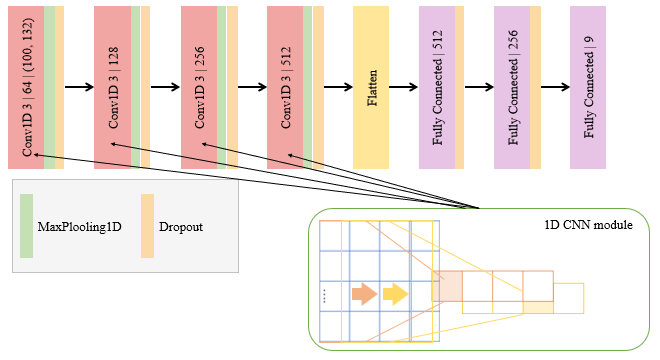
\includegraphics[width=\linewidth]{bab3/ar_CNNArch.png}
	\caption{Architecture of CNN that used in this research.}
	\label{fig:CNNArch}
\end{figure}

The model consists of several main components. First, there are four 1D convolution layers (Conv1D) with a kernel of size 3, which have 64, 128, 256, and twice 512 filters, respectively. These layers are responsible for extracting features from the input data. After each convolution layer, there is a MaxPooling1D layer that is used to reduce the dimensionality of the data and capture the main features, helping in reducing the data size and computation. In addition, multiple convolution layers are followed by a dropout layer to prevent overfitting by randomly disabling a number of units in the network during training. The output of the convolution and pooling layers is then flattened using the Flatten layer, turning the data into a 1D vector that can be fed to the fully connected layer. There are three fully connected layers in this architecture, with 512, 256, and 9 units respectively, where the last layer is typically used as the output layer for classification into 9 classes.
% Model ini terdiri dari beberapa komponen utama. Pertama, terdapat lima lapisan konvolusi 1D (Conv1D) dengan kernel ukuran 3, yang berturut-turut memiliki 64, 128, 256, dan dua kali 512 filter. Lapisan-lapisan ini bertugas mengekstrak fitur dari data input. Setelah setiap lapisan konvolusi, terdapat lapisan MaxPooling1D yang digunakan untuk mengurangi dimensi data dan menangkap fitur utama, membantu dalam mengurangi ukuran data dan komputasi. Selain itu, beberapa lapisan konvolusi diikuti oleh lapisan dropout untuk mencegah overfitting dengan secara acak menonaktifkan sejumlah unit dalam jaringan selama pelatihan. Output dari lapisan konvolusi dan pooling kemudian diratakan menggunakan lapisan Flatten, mengubah data menjadi vektor 1D yang dapat diumpankan ke lapisan fully connected. Terdapat tiga lapisan fully connected dalam arsitektur ini, dengan masing-masing 512, 256, dan 9 unit, di mana lapisan terakhir biasanya digunakan sebagai lapisan output untuk klasifikasi ke dalam 9 kelas.

Overall, this architecture is designed to process sequential data by extracting features through a convolution layer, reducing dimensionality by pooling, preventing overfitting with dropout, and performing classification through a fully connected layer. This combination makes the 1D CNN model very suitable for tasks such as signal analysis, text processing, or other sequential data.
% Secara keseluruhan, arsitektur ini dirancang untuk mengolah data sekuensial dengan cara mengekstrak fitur melalui lapisan konvolusi, mengurangi dimensi dengan pooling, mencegah overfitting dengan dropout, dan melakukan klasifikasi melalui lapisan fully connected. Kombinasi ini membuat model 1D CNN sangat cocok untuk tugas-tugas seperti analisis sinyal, pemrosesan teks, atau data sekuensial lainnya.


\subsection{LSTM Architecture}

Another architecture used is the LSTM. This architecture is a further development of the traditional RNN. LSTMs address the traditional RNN problems of vanishing gradient and long-term dependencies. LSTMs are able to remember important information for a longer period of time than traditional RNNs. The data used in this research is time series data with long temporal patterns, making LSTM suitable for this dataset.
% Arsitektur lain yang digunakan adalah LSTM. Arsitektur ini merupakan pengembangan lebih lanjut dari RNN tradisional. LSTM menangani masalah RNN tradisional terkait vanishing gradient dan long-term dependencies. LSTM mampu mengingat informasi penting untuk jangka waktu lebih panjang dibanding RNN biasa. Data yang digunakan pada penelitian ini merupakan data time series dengan pola temporal panjang, menjadikan LSTM cocok untuk dataset ini. 

\begin{figure}[h!]
	\centering
	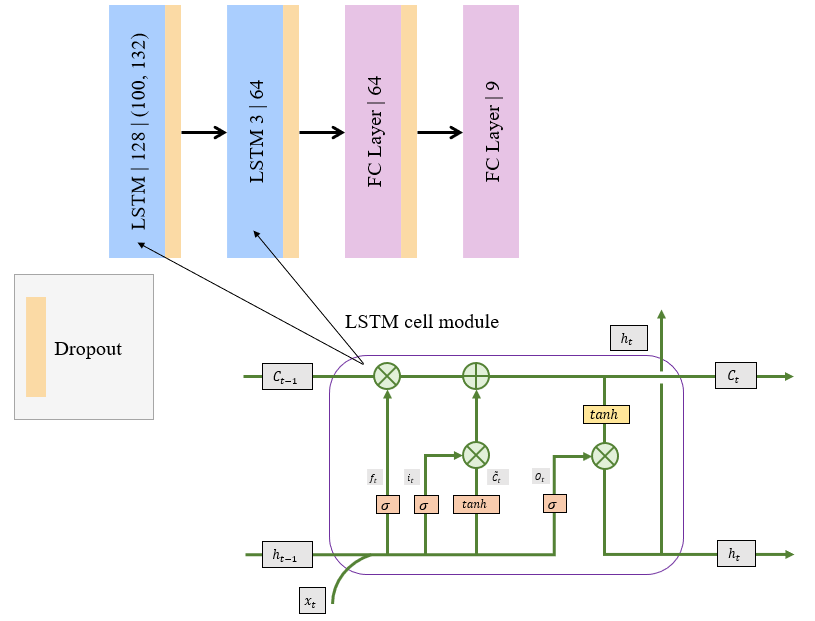
\includegraphics[width=\linewidth]{bab3/ar_LSTMArch.png}
	\caption{Architecture of LSTM that used in this research.}
	\label{fig:LSTMArch}
\end{figure}

The architecture shown in figure \ref{fig:LSTMArch} is a Long Short-Term Memory (LSTM) model used for processing sequential or time-based data. This model consists of several main components. First, there are two LSTM layers. The first LSTM layer has 128 units and accepts inputs with dimensions (100, 132), followed by a dropout layer to prevent overfitting by randomly disabling a number of units in the network during training. The second LSTM layer has 64 units and is also followed by a dropout layer. This LSTM layer is used to capture long-term dependencies in sequential data.
% Arsitektur yang ditunjukkan pada gambar \ref{fig:LSTMArch} adalah model Long Short-Term Memory (LSTM) yang digunakan untuk memproses data sekuensial atau data berbasis waktu. Model ini terdiri dari beberapa komponen utama. Pertama, terdapat dua lapisan LSTM. Lapisan LSTM pertama memiliki 128 unit dan menerima input dengan dimensi (100, 132), diikuti oleh lapisan dropout untuk mencegah overfitting dengan secara acak menonaktifkan sejumlah unit dalam jaringan selama pelatihan. Lapisan LSTM kedua memiliki 64 unit dan juga diikuti oleh lapisan dropout. Lapisan LSTM ini digunakan untuk menangkap dependensi jangka panjang dalam data sekuensial.

After the LSTM layer, the output is flattened and fed to two fully connected (FC) layers. The first fully connected layer has 64 units, while the second fully connected layer has 9 units, which is usually used as the output layer for classification into 9 classes. The diagram on the bottom right shows the LSTM cell module in detail, which illustrates the internal mechanism of the LSTM cell including the input gate (\(i_t\)), forgetting gate (\(f_t\)), and output gate (\(o_t\)), as well as how the state cells (\(C_t\)) are updated through sigmoid operation (\(\sigma\)) and tanh activation function.
% Setelah lapisan LSTM, output diratakan dan diumpankan ke dua lapisan fully connected (FC). Lapisan fully connected pertama memiliki 64 unit, sementara lapisan fully connected kedua memiliki 9 unit, yang biasanya digunakan sebagai lapisan output untuk klasifikasi ke dalam 9 kelas. Diagram di kanan bawah menunjukkan modul sel LSTM secara detail, yang menggambarkan mekanisme internal dari sel LSTM termasuk gerbang input (\(i_t\)), gerbang melupakan (\(f_t\)), dan gerbang output (\(o_t\)), serta bagaimana sel-sel status (\(C_t\)) diperbarui melalui operasi sigmoid (\(\sigma\)) dan fungsi aktivasi tanh. 

The architecture's overall goal is to handle and evaluate sequential data by utilizing the fully connected layer to do classification, the LSTM layer to capture temporal information, and dropout to minimize overfitting. Because of this combination, the LSTM model performs exceptionally well in applications like signal processing, time series prediction, and text analysis.
% Secara keseluruhan, arsitektur ini dirancang untuk memproses dan menganalisis data sekuensial dengan menangkap informasi temporal menggunakan lapisan LSTM, mencegah overfitting dengan dropout, dan melakukan klasifikasi melalui lapisan fully connected. Kombinasi ini membuat model LSTM sangat efektif dalam tugas-tugas seperti analisis teks, prediksi deret waktu, dan pemrosesan sinyal.

\subsection{CNN-LSTM Architecture}
\begin{figure}[h!]
	\centering
	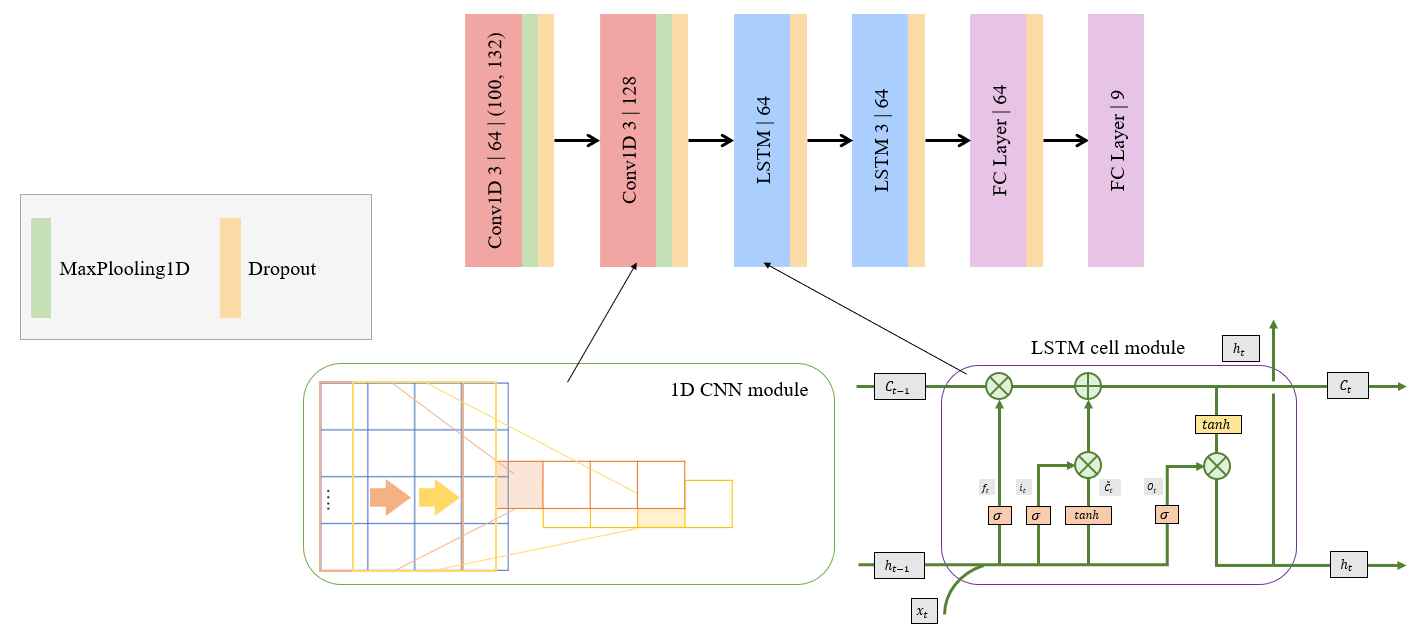
\includegraphics[width=\linewidth]{bab3/ar_CNNLSTMArch.png}
	\caption{Architecture of CNN-LSTM that used in this research.}
	\label{fig:CNNLSTMArch}
\end{figure}

Our proposed CNN-LSTM architecture starts with two consecutive one-dimensional convolution (Conv1D) layers, each followed by a one-dimensional max pooling (MaxPooling1D) layer. The first Conv1D layer has the objective of capturing local features of the input sequence, with the convolution kernel applying a non-linear filter on a subset of the data. After each convolution layer, the MaxPooling1D layer is used to reduce the output dimension and control overfitting by taking the maximum value of a small subset of the convolution layer output. Next, the architecture continues with two Long Short-Term Memory (LSTM) layers followed by a dropout layer. The first LSTM layer serves to capture temporal dependencies in the data sequence, while the subsequent dropout layer helps reduce overfitting by randomly disabling units during training. The second LSTM layer deepens the model's understanding of complex sequence patterns, followed by another dropout layer for additional regulation. Then, the model ends with two Dense layers, each of which is followed by a dropout layer. The first Dense layer with ReLU activation function serves to combine the learned features and apply them to a lower output dimension. The last dropout layer ensures that the model still generalizes well to data that has never been seen. Finally, a second Dense layer with a softmax activation function is used to generate the final prediction that represents the probability of each possible class. The output of this model is a model that can classify 9 classes of elderly exercise activities.

\subsection{Deep CNN-LSTM Architecture}

\begin{figure}[h!]
	\centering
	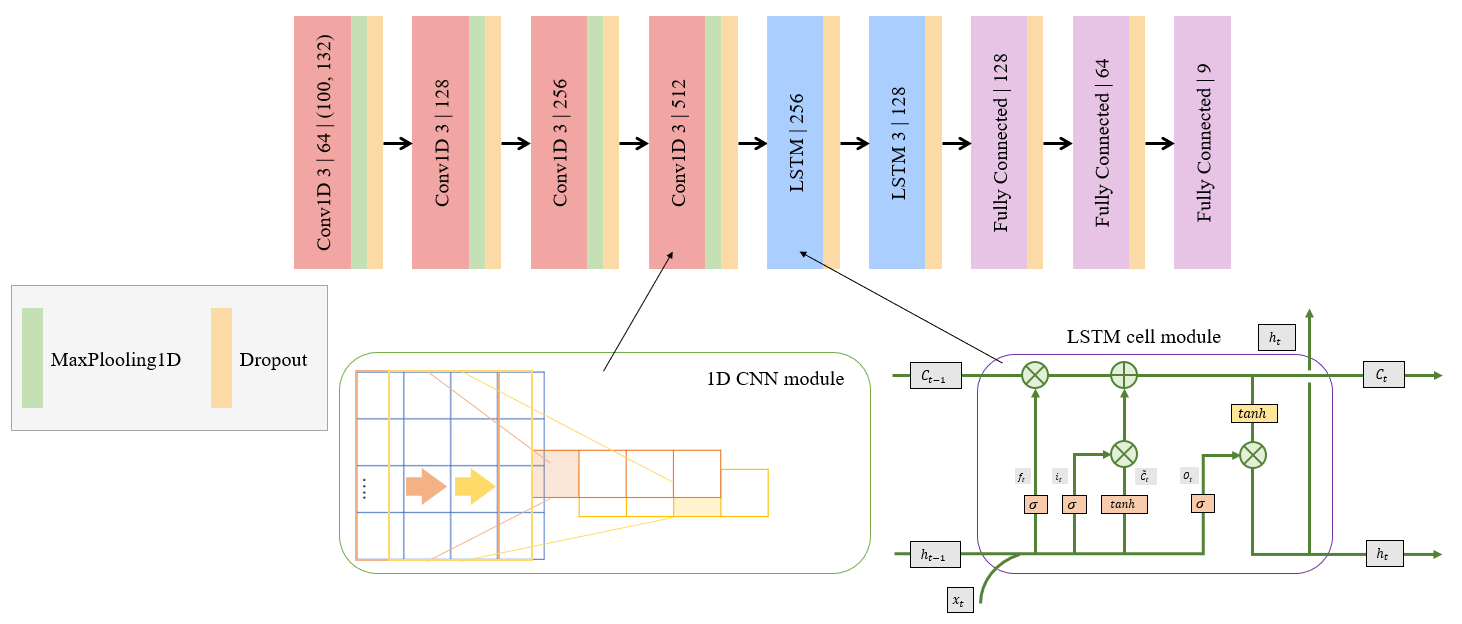
\includegraphics[width=\linewidth]{bab3/ar_DeepCNNLSTMArch.png}
	\caption{Architecture of Deep CNN-LSTM that used in this research.}
	\label{fig:DeepCNNLSTMArch}
\end{figure}

The architecture shown in figure \ref{fig:DeepCNNLSTMArch} is a combination of a one-dimensional Convolutional Neural Network (CNN) (1D CNN) and Long Short-Term Memory (LSTM) model designed to process sequential or time-based data, such as signals or text data. The model consists of several main components that work sequentially.
% Arsitektur yang ditunjukkan pada gambar \ref{fig:DeepCNNLSTMArch} adalah kombinasi dari model Convolutional Neural Network (CNN) satu dimensi (1D CNN) dan Long Short-Term Memory (LSTM) yang dirancang untuk memproses data sekuensial atau data berbasis waktu, seperti sinyal atau data teks. Model ini terdiri dari beberapa komponen utama yang bekerja secara berurutan.

The first layer consists of several 1D convolution layers (Conv1D) with a size 3 kernel. The first convolution layer takes input with dimensions (100, 132) and has 64 filters. A Conv1D layer with 128 filters is next, then a layer with 256 filters, and two layers with 512 filters apiece. After each of these convolution layers, there is a dropout layer to avoid overfitting and a MaxPooling1D layer to reduce the dimensionality of the data and capture important characteristics.
% Pertama, terdapat beberapa lapisan konvolusi 1D (Conv1D) dengan kernel ukuran 3. Lapisan konvolusi pertama memiliki 64 filter dan menerima input dengan dimensi (100, 132). Selanjutnya, terdapat lapisan Conv1D dengan 128 filter, diikuti dengan lapisan Conv1D dengan 256 filter, dan dua lapisan Conv1D masing-masing dengan 512 filter. Setiap lapisan konvolusi ini diikuti oleh lapisan MaxPooling1D untuk mengurangi dimensi data dan menangkap fitur utama serta lapisan dropout untuk mencegah overfitting.

The output of the convolution layer is sent to the LSTM layer following the feature extraction procedure using the convolution layer. This architecture consists of two LSTM layers, the first with 256 units and the second with 128 units. The long-term dependencies in sequential data are captured by these LSTM layers.
% Setelah proses ekstraksi fitur dengan lapisan konvolusi, output dari lapisan konvolusi diteruskan ke lapisan LSTM. Terdapat dua lapisan LSTM dalam arsitektur ini: lapisan LSTM pertama memiliki 256 unit, dan lapisan LSTM kedua memiliki 128 unit. Lapisan LSTM ini bertugas untuk menangkap dependensi jangka panjang dalam data sekuensial.

The output of the LSTM layer is supplied to three fully connected (FC) layers after being flattened. The output layer for categorization into nine classes is typically the third fully connected layer, which has nine units. The first fully connected layer has 128 units, the second fully connected layer has 64 units, and so on.
% Setelah lapisan LSTM, outputnya diratakan dan diumpankan ke tiga lapisan fully connected (FC). Lapisan fully connected pertama memiliki 128 unit, lapisan fully connected kedua memiliki 64 unit, dan lapisan fully connected ketiga memiliki 9 unit, yang biasanya digunakan sebagai lapisan output untuk klasifikasi ke dalam 9 kelas.

% Diagram di bagian bawah gambar menunjukkan detail dari modul sel LSTM, yang menggambarkan mekanisme internal dari sel LSTM termasuk gerbang input (\(i_t\)), gerbang melupakan (\(f_t\)), dan gerbang output (\(o_t\)), serta bagaimana sel-sel status (\(C_t\)) diperbarui melalui operasi sigmoid (\(\sigma\)) dan fungsi aktivasi tanh.













% This section explains the testing of elderly activity detection compared to the LSTM-trained model. The obtained model is then tested in real-time for each corresponding movement. The testing results are evaluated using mean Average Precision (mAP). mAP is the average of the model's Average Precision (AP), as shown in equation \ref{equ:mAP}. Performance evaluation of an object detection model can be measured using mAP, which is constrained by the Intersection over Union (IoU) of the detection results.

% \begin{equation}
% 	\begin{aligned}
% 		\label{equ:mAP}
% 		mAP = \frac{1}{n}\sum_{k=n}^{k=1}AP_k
% 	\end{aligned}
% \end{equation}

% ($R^2$)\cite{dormann2013collinearity} as shown in (\ref{equ:VIF}):
% \begin{equation}
% 	VIF(\ell, S):=\frac{1}{1-R^{2}(\ell,S)}
% 	\label{equ:VIF}
% \end{equation}

% \begin{equation}
% 	\label{equ:r2}
% 	\begin{aligned}
% 		R^2= 1 - \frac{\sum(y_i-\hat{y}_i)^2}{\sum(y_i-\bar{y}_i)^2}
% 	\end{aligned}
% \end{equation}

% \begin{equation}
% 	\label{equ:rmse}
% 	\begin{aligned}
% 		RMSE_{(y,\hat{y})} = \sqrt{\frac{1}{n_{samples}}\sum_{i=0}^{n_{samples}-i}(y_i-\hat{y}_i)^2}
% 	\end{aligned}
% \end{equation}

% \begin{equation}
% 	\label{equ:mape}
% 	\begin{aligned}
% 		MAPE_{(y,\hat{y})} = \frac{1}{n_{samples}}\sum_{i=0}^{n_{samples}-i}\left | \frac{y_i-\hat{y}_i}{y_i}*100 \right |
% 	\end{aligned}
% \end{equation}

% \begin{equation}
% 	\label{equ:explanation}
% 	e=f(b,x)
% \end{equation}

% $F$ $\mathcal{L}$

% ($f_{S\cup {i}}$)

% \begin{equation}
% 	\label{equ:shapley}
% 	\phi_i=\underset{S\subseteq F_{i}}{\sum} \frac{|S|!(|F|-|S|-1)!}{|F|!}[f_{S\cup {i}} (x_{S\cup {i}}) -  f_S(x_S)]
% \end{equation}

% \begin{eqnarray}
% 	\label{equ:MinMaxScaler}
% 	X_{std}= \frac{X - X_{min}(axis=0)}{X_{max}(axis=0)}\\
% 	X_{scaled} = X_{std} * (max - min) + min
% \end{eqnarray}

% % numbering: itemize, enumerate, description
% \begin{description}
% 	\item[a]asfa
% 	\item[s] asfaaa
% \end{description}

% % contoh equation
% \begin{align}
% 	y & = 1-3-4-4\nonumber \\
% 	  & = 1-3-4\nonumber   \\
% 	  & = 1-3
% \end{align}

	\cleardoublepage
	\chapter{RESULT AND DISCUSSION}
\label{sec:chap4_result}
% Please add the following required packages to your document preamble:
% \usepackage{multirow}
% \usepackage[table,xcdraw]{xcolor}
% If you use beamer only pass "xcolor=table" option, i.e. \documentclass[xcolor=table]{beamer}
\section{PhysioExercise Dataset}
\label{sec4:dataset_evaluation}
This section is about the collected dataset and its details. Our dataset consists of 9 classes according to the predefined elderly exercise activities. Within each class, videos were taken as described in Methodology. We take several physical issues that are common in the elderly. There are three categories of physical issues that we take for this dataset, i.e., frozen shoulder, tennis elbow, and knee pain. In brief, frozen shoulder is a common condition affecting the elderly, characterized by pain and limited movement in the shoulder joint. The second physical problem is tennis elbow. Tennis elbow is a condition characterized by pain and tenderness on the outside of the elbow. The knee as the main support of the body often experiences knee pain problems.
% Bagian ini menjelaskan dataset yang telah dikumpulkan dan rinciannya. Dataset kami terdiri atas 9 kelas sesuai dengan aktivitas latihan elderly yang ditentukan sebelumnya. Dalam setiap kelasnya, video diambil berdasarkan yang telah dijelaskan pada bagian XX. Kami mengambil beberapa masalah fisik yang awam terjadi pada elderly. Terdapat tiga kategori masalah fisik yang kami ambil untuk dataset kali ini, yaitu frozen shoulder, tennis elbow, dan knee pain. Secara singkat, frozen shoulder adalah kondisi umum yang mempengaruhi elderly, ditandai dengan nyeri dan gerakan terbatas pada sendi bahu. Masalah fisik yang kedua adalah tennis elbow. Tennis elbow adalah kondisi yang ditandai dengan rasa nyeri dan nyeri tekan pada bagian luar siku. Adapun lutut sebagai penopang utama badan seringkali mengalami masalah knee pain.

\begin{table}[h!]
	\caption{Physiotherapy exercises used as dataset classes and the distributions.}
	\label{tab:class-dataset}
	\centering
	\begin{tabularx}{\textwidth}{|l|X|r|r|}
		\hline
		\textbf{Physical Issue}                            & \textbf{Physiotherapy \newline Exercise} & \textbf{Total Person} & \textbf{Total Video} \\ \hline
		\multirow{4}{*}{Frozen Shoulder}
		                                                   & Adduction \newline Abduction             & 5                     & 206                  \\ \cline{2-4}
		                                                   & Left Arm \newline Circumduction          & 5                     & 227                  \\ \cline{2-4}
		                                                   & Right Arm \newline Circumduction         & 6                     & 227                  \\ \cline{2-4}
		                                                   & Shoulder Flexion \newline Tension        & 7                     & 229                  \\ \hline
		Tennis Elbow                                       & Elbow Flexion \newline Tension           & 5                     & 219                  \\ \hline
		\multirow{4}{*}{Knee Pain}
		                                                   & Left Knee Flexion \newline Extension     & 5                     & 195                  \\ \cline{2-4}
		                                                   & Right Knee Flexion \newline Extension    & 5                     & 195                  \\ \cline{2-4}
		                                                   & Left Leg Flexion \newline Extension      & 5                     & 206                  \\ \cline{2-4}
		                                                   & Right Leg Flexion \newline Extension     & 5                     & 195                  \\ \hline
		\multicolumn{3}{|l|}{\textbf{Total video dataset}} & 1899                                                                                    \\ \hline
	\end{tabularx}
\end{table}

Based on the three physical issues of the elderly that have been mentioned, we determine the exercise activities. Table \ref{tab:class-dataset} shows the exercise activity classes used in this work. There are a total of 9 kinds of activities performed to solve the above physical issues. There are 4 kinds of exercises to prevent frozen shoulder problems. The activities are adduction abduction, left arm circumduction, right arm circumduction, and shoulder flexion tension. These four exercises are movements that use the shoulder as the main focus in doing them. We take one exercise activity to prevent tennis elbow problems, which is elbow flexion tension. This movement uses the arm as the main focus. Finally, there are 4 types of training activities to prevent knee pain problems. The training activities are left knee flexion extension, right knee flexion extension, left leg flexion extension, and right leg flexion extension. Left knee flexion extension and right knee flexion extension are movements performed in a sitting position with the thighs and calves forming a \ang{90}. In this movement an elderly person will try to straighten their calves forward. The left leg flexion extension and right leg flexion extension are performed in a standing position. An elderly person will try to bend their knees backwards so that the thighs and knees form a \ang{90} angle.
% Dari tiga masalah fisik elderly yang telah disebutkan, aktifitas latihan kami tentukan. Tabel 1 menunjukkan kelas aktifitas latihan yang digunakan pada pekerjaan ini. Total terdapat 9 macam aktifitas yang dilakukan untuk penyelesaian permasalahan fisik di atas. Terdapat 4 macam latihan untuk mencegah permasalahan frozen shoulder. Aktifitas yang dimaksud adalah adduction abduction, left arm circumduction, right arm circumduction, dan shoulder flexion tension. Keempat latihan ini merupakan gerakan yang menggunakan bahu sebagai tumpuan utama dalam melakukannya. Kami mengambil satu aktifitas latihan untuk mencegah masalah tennis elbow, yaitu elbow flexion tension. Gerakan ini menggunakan lengan sebagai tumpuan utama. Terakhir, terdapat 4 jenis aktifitas latihan untuk mencegah permasalahan knee pain. Aktifitas latiha yang dilakukan adalah left knee flexion extension, right knee flexion extension, left leg flexion extension, dan right leg flexion extension. Left knee flexion extension dan right knee flexion extension merupakan gerakan yang dilakukan dalam posisi duduk dengan paha dan betis membentuk sudut \ang{90}. Pada gerakan ini seorang elderly akan berusaha untuk meluruskan betisnya ke depan. Adapun left leg flexion extension dan right leg flexion extension dilakukan dalam posisi berdiri. Seorang elderly akan berusaha menekuk lututnya ke belakang sehingga paha dan lutut membentuk sudut \ang{90}.

\begin{figure}[h!]
	\centering
	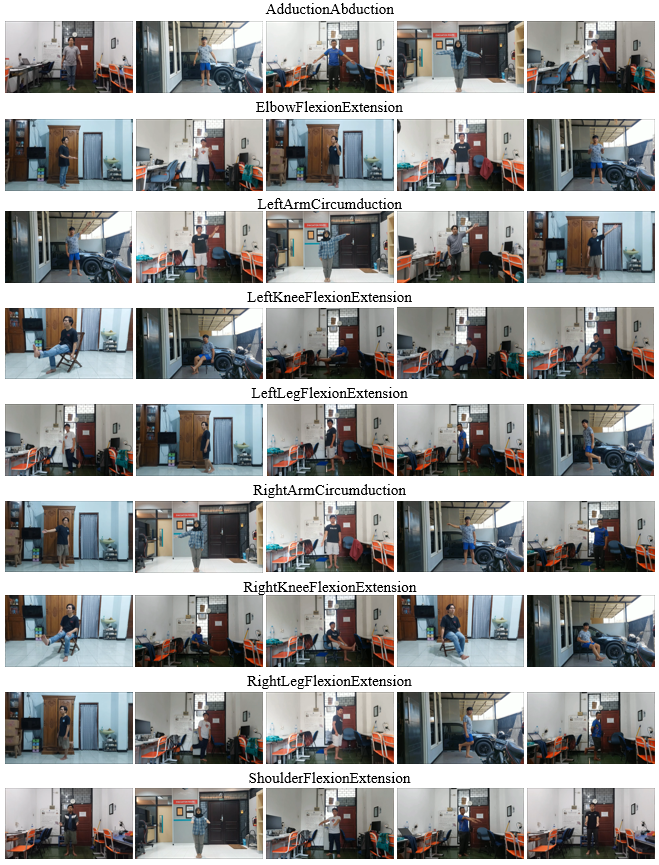
\includegraphics[width=1\textwidth]{bab4/ar_DatasetDist.png}
	\caption{Dataset distribution of PhysioExercise.}
	\label{fig:DatasetDistribution}
\end{figure}

We used multiple subjects to conduct the data acquisition process. There were at least 7 different subjects for this data acquisition process. The age range of the subjects in this work is between 21 to 36 years old. A wide age range was chosen because the feature used for training is pose estimation keypoint extraction. Moreover, these subjects are in good health, which makes it easier to capture the right movements in accordance with the physiotherapist's recommendations. There are a total of 1899 videos in this dataset.
% Kami menggunakan beberapa subjek untuk melakukan proses akuisisi data. Terdapat setidaknya 7 subjek berbeda untuk proses akuisisi data ini. Rentang usia subjek pada pekerjaan ini antara usia 21 hingga 36 tahun. Rentang usia yang beragam dipilih karena fitur yang digunakan untuk pelatihan adalah ekstraksi keypoint estimasi pose. Moreover, subjek-subjek ini dalam kondisi sehat, sehingga memudahkan dalam pengambilan gerakan yang tepat dan sesuai dengan anjuran physiotherapist. Total terdapat 1899 video pada dataset ini.

Figure \ref{fig:DatasetDistribution} shows the diversity and distribution of the dataset for each class. The dataset is organized to have a variety of capture angles, such as front view, left view, and right view. The capture angle for each view was varied to close to a \ang{90} relative to the front view. In addition, the video illumination level was also varied. We took the dataset in several time situations, such as morning, afternoon, evening, and night. Some videos have normal light and others have low light. The diverse lighting is intended to make the model adaptable to various lighting conditions. We took this dataset in several different environments, namely a laboratory environment and a home environment. The home environment was chosen to match the use of the model that will be used by the elderly in their respective homes.
% Gambar XX menunjukkan diversitas dan distribusi dari dataset untuk setiap kelasnya. Dataset diatur agar memiliki variasi sudut pengambilan, seperti front view, left view, dan right view. Sudut pengambilan untuk masing-masing pandangan dibuat beragam hingga mendekati sudut 90 relatif terhadap front view. Selain itu, tingkat penerangan video juga beragam. Kami mengambil dataset dalam beberapa situasi waktu, seperti pagi hari, siang hari, sore hari, dan malam hari. Sebagian video memiliki normal light dan sebagian sisanya memiliki low light. Pencahayaan yang beragam ditujukkan agar model yang dihasilkan dapat beradaptasi untuk berbagai kondisi penerangan. Kami mengambil dataset ini dalam beberapa macam lingkungan, yaitu lingkungan laboratorium dan lingkungan rumah. Macam lingkungan rumah dipilih untuk menyesuaikan dengan penggunaan model yang akan digunakan oleh elderly di rumah masing-masing.


% Setiap kelasnya memiliki data sebanyak 150 video. Sejak pemanfaatan keypoints sebagai fitur dalam pelatihan, video-video tersebut harus dipotong menjadi urutan-urutan citra yang merepresentasikan aktivitas latihan elderly. Dataset kami saat ini memiliki keragaman durasi video mulai dari 5 - 16 detik. Satu video kami convert menjadi urutan-urutan citra sebanyak 250 citra. Kami membagi sebuah video menjadi 250 frame secara merata dari awal frame hingga akhir frame agar merepresentasikan urutan aktivitas latihan elderly. Sejak setiap estimasi pose memiliki 33 keypoints dan 150 data setiap kelasnya, total keypoint yang diekstraksi setiap kelasnya sebesar 1350 keypoints. Total keseluruhan keypoints yang diekstrak untuk 9 kelas adalah 44500. 

\section{Video Frame Extraction}
\label{se4:VIdeoExtraction}

\begin{figure}[h!]
	\centering
	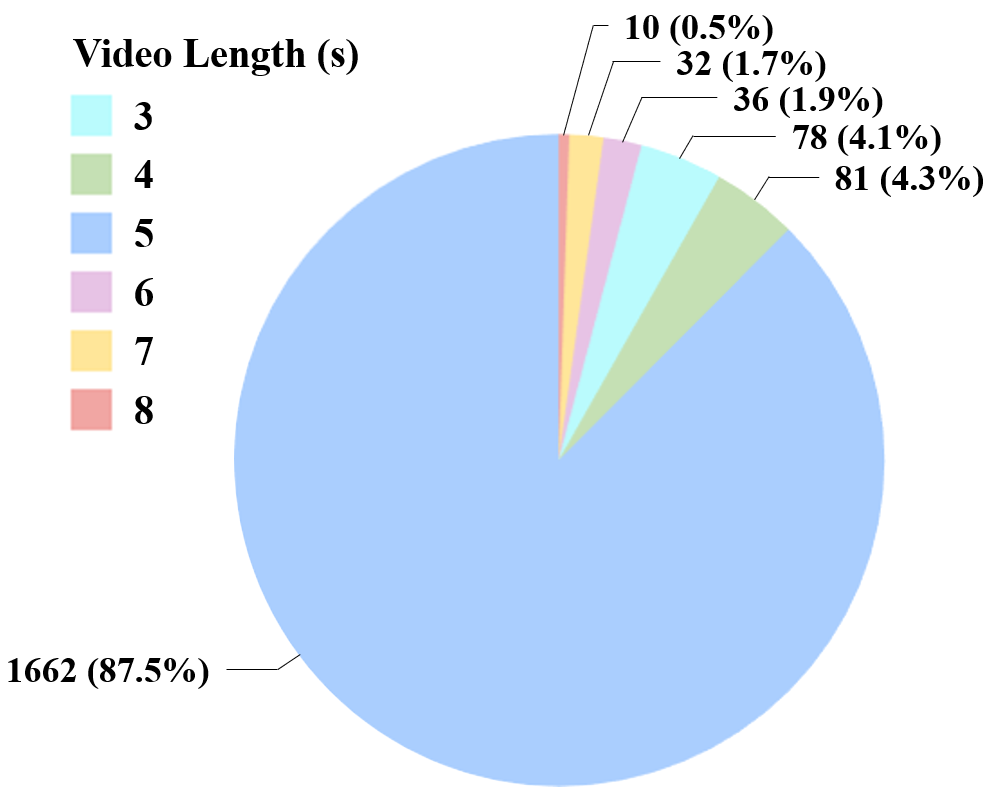
\includegraphics[width=0.6\textwidth]{bab4/ar_VideoLength.png}
	\caption{Statistics for the length distribution of our video dataset. Videos with a length of 5 seconds are the most recorded.}
	\label{fig:VideoLengthDistribution}
\end{figure}

The acquired dataset is a set of exercise activity videos for the elderly. Since the Mediapipe framework performs frame by frame pose estimation, our data must first go through a video frame extraction process. The video data we have is a short duration video. Figure \ref{fig:VideoLengthDistribution} shows the distribution of video length in the dataset. The duration of the videos we collected is in the range of 3 to 8 seconds. The duration with the least amount of data is 3 seconds, with only a total of 10 videos or 0.5\% of the overall data. In contrast, the duration with the most data is 5 seconds, with a total of 1662 videos or 87.5\% of the overall data.
% Dataset yang telah diakuisisi adalah sekumpulan video aktifitas latihan untuk elderly. Sejak framework Mediapipe melakukan estimasi pose frame by frame, data yang kami miliki harus melalui proses video frame extraction terlebih dahulu. Data video yang kami miliki merupakan video dengan durasi yang pendek. Gambar \ref{fig:VideoLengthDistribution} menunjukkan pesebaran panjang video pada dataset. Durasi dari video yang kami kumpulkan berada pada rentang 3 hingga 8 detik. Durasi dengan jumlah data paling sedikit adalah 3 detik, dengan hanya total 10 video saja atau 0.5\% dari keseluruhan data. Sebaliknya, Durasi dengan jumlah data paling banyak adalah 5 detik, dengan total 1662 video atau 87.5\% dari keseluruhan data.

Video frame extraction is done by dividing each video into 100 frames. This number of frames is determined so that not too many frames are extracted (12 - 30 FPS). We extract the video into fewer frames because we want to avoid frames that have too much motion blur. Motion blur in the context of pose estimation can blur the information carried, resulting in frames that are not good for deep learning training data. On the other hand, we also keep the overall information in a video intact. Within the 100 frames for a video, we spread them evenly throughout the video from beginning to end. So no information is left out in this video frame extraction.
% Video frame extraction dilakukan dengan membagi setiap video menjadi 100 frames. Jumlah frame ini ditentukan agar tidak terlalu banyak frame yang diekstrak (1 - 5 FPS). Kami mengekstrak video menjadi lebih sedikit frame karena kami ingin menghindari frame yang memiliki terlalu banyak motion blur. Motion blur dalam konteks estimasi pose dapat membuat informasi yang dibawa menjadi kabur, mengakibatkan frame yang tidak bagus untuk menjadi data pelatihan deep learning. Di lain sisi, kami juga tetap menjaga keseluruhan informasi dalam satu video tetap utuh. Dalam 100 frames untuk sebuah video, kami menyebar rata sepanjang video dari awal hingga akhir. Jadi tidak ada informasi yang tertinggal dalam ekstraksi frame video ini.

\section{Keypoint Ekstraction}
\label{sec4:KeypointExtraction}
This stage is the stage to extract keypoint features from human pose estimation. Keypoint extraction is performed using the Mediapipe framework. The keypoint extraction process that we performed using the MediaPipe framework successfully produced high-quality keypoint data from each processed video frame. Figure \ref{fig:KeypointViz} shows an example of keypoint extraction results from a frame, where keypoints are clearly identified at key positions of the subject's body. This result demonstrates the effectiveness of MediaPipe in extracting pose information with precision, even in activities that involve fast and complex movements.
% Tahap ini merupakan tahap untuk mengekstrak fitur keypoint dari estimasi pose manusia. Ekstraksi keypoint dilakukan menggunakan framework Mediapipe. Proses ekstraksi keypoint yang kami lakukan menggunakan framework MediaPipe berhasil menghasilkan data keypoint yang berkualitas tinggi dari setiap frame video yang diproses. Gambar \ref{fig:KeypointViz} menunjukkan contoh hasil ekstraksi keypoint dari sebuah frame, di mana keypoint teridentifikasi dengan jelas pada posisi-posisi penting tubuh subjek. Hasil ini memperlihatkan efektivitas MediaPipe dalam mengekstrak informasi pose dengan presisi, bahkan pada aktivitas yang melibatkan gerakan cepat dan kompleks.

\begin{figure}[h!]
	\centering
	\subfloat[]{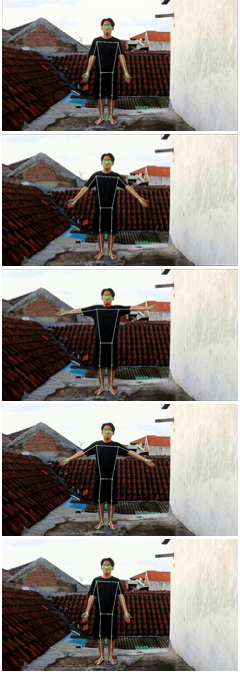
\includegraphics[width=0.33\textwidth]{bab4/ar_Key1.png}}
	\subfloat[]{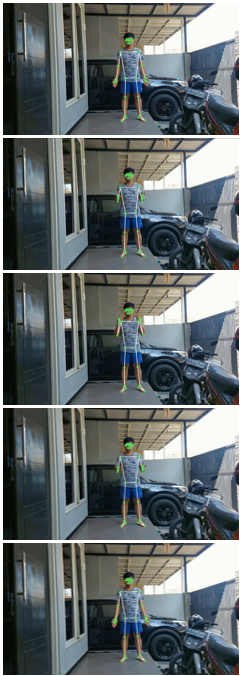
\includegraphics[width=0.33\textwidth]{bab4/ar_Key2.png}}
	\subfloat[]{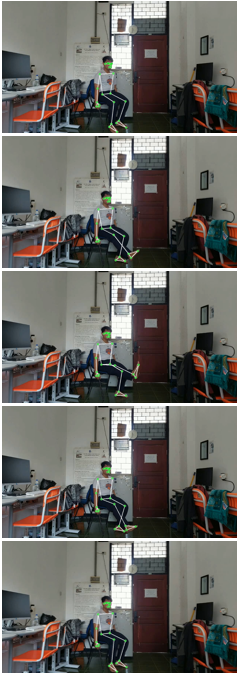
\includegraphics[width=0.33\textwidth]{bab4/ar_Key3.png}}
	\caption{Examples of pose estimation results using mediapipe for exercise activity types (a) adduction abduction, (b) elbow flexion extension, and (c) right knee flexion extension.}
	\label{fig:KeypointViz}
\end{figure}

Each extracted frame provides comprehensive information on the type of exercise activity performed by the subject. By sequentially extracting keypoints for each frame, we were able to build a detailed and dynamic dataset that reflects the entire range of motion in the activity. From this dataset, we were able to see how the position and orientation of the body changed over time, providing deep insight into the biomechanical characteristics of each exercise activity.
% Setiap frame yang diekstrak menyajikan informasi yang lengkap mengenai jenis aktivitas latihan yang dilakukan oleh subjek. Dengan mengekstrak keypoint untuk setiap frame secara berurutan, kami mampu membangun dataset yang mendetail dan dinamis, yang merefleksikan seluruh rangkaian gerakan dalam aktivitas tersebut. Dari dataset ini, kami dapat melihat bagaimana posisi dan orientasi tubuh berubah sepanjang waktu, memberikan wawasan mendalam tentang karakteristik biomekanik dari masing-masing aktivitas latihan.

From the keypoint extraction process, we generate a data array that describes the keypoint position in three dimensions (\(x,y,z)\) and the confidence score. This array shows the (\(x)\), (\(y)\) and (\(z)\) positions for each keypoint with their associated confidence scores, where these scores indicate the accuracy of keypoint detection by the model. The use of three-dimensional data allows us to perform a more detailed analysis of the motion performed, including the depth of motion that cannot be achieved with only two-dimensional data.
% Dari proses ekstraksi keypoint, kami menghasilkan array data yang menggambarkan posisi keypoint dalam tiga dimensi (\(x,y,z)\) dan skor kepercayaan. Array ini menunjukkan posisi (\(x)\), (\(y)\) dan (\(z)\) untuk setiap keypoint dengan skor kepercayaan yang terkait, di mana skor ini mengindikasikan keakuratan deteksi keypoint oleh model. Penggunaan data tiga dimensi memungkinkan kami untuk melakukan analisis yang lebih detil terhadap gerakan yang dilakukan, termasuk kedalaman gerakan yang tidak dapat dicapai hanya dengan data dua dimensi.

\section{Data Training Preparation}
\label{sec:DataTrainingPreparation}
\begin{figure}[]
	\centering
	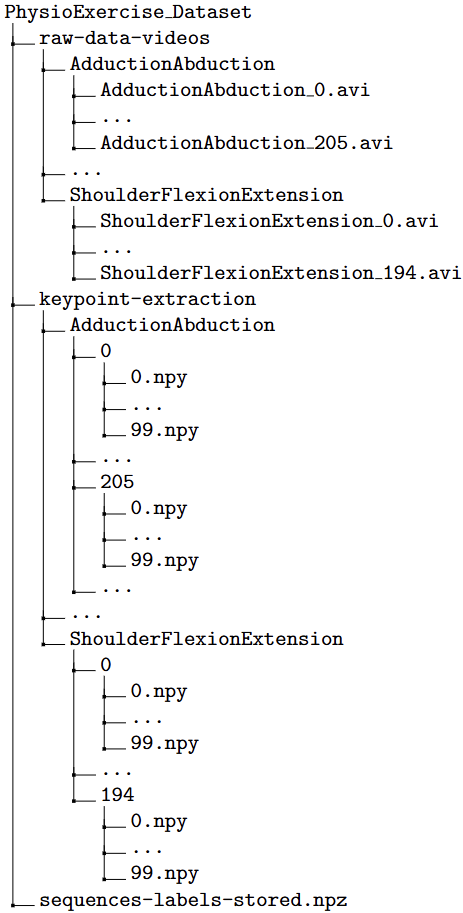
\includegraphics[width=0.7\textwidth]{bab4/ar_DataStructure.png}
	\caption{Data structure of PhysioExercise dataset.}
	\label{fig:DataStructure}
\end{figure}

This section describes the data structure of the dataset that will be used for the training process. The PhysioExercise dataset consists of raw data and data extracted from keypoints using the Mediapipe framework. Figure \ref{fig:DataStructure} shows the data structure of the dataset. The data used in this training is a collection of arrays containing information from images. To get a collection of arrays, the process goes through several stages. The first stage is to collect all video data into a folder. These video data are the raw data that will be extracted from the video frames and keypoints. The amount of data in each class is different, as shown in table \ref{tab:class-dataset}.
% Bagian ini menjelaskan struktur data dari dataset yang akan digunakan untuk proses pelatihan. Dataset PhysioExercise terdiri dari data mentah dan data hasil ekstraksi keypoint menggunakan framework Mediapipe. Gambar \ref{fig:DataStructure} menunjukkan struktur data dari dataset. Data yang digunakan dalam pelatihan ini adalah kumpulan data array yang berisikan informasi dari citra. Untuk mendapatkan kumpulan array, proses dilalui dalam beberapa tahapan. Tahapan pertama adalah mengumpulkan seluruh data video ke dalam sebuah folder. Data-data video ini merupakan data mentah yang akan diekstrak frame video dan keypoint-nya. Jumlah dari data pada setiap kelasnya berbeda-beda, seperti yang ditunjukkan pada tabel \ref{tab:class-dataset}. 

\begin{figure}[h!]
	\centering
	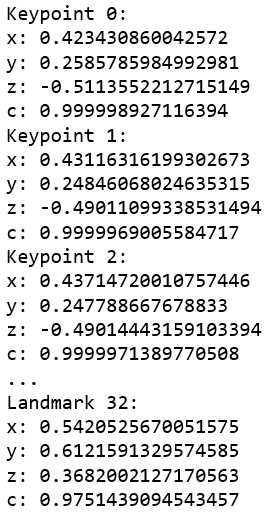
\includegraphics[width=0.33\textwidth]{bab4/ar_KeypointExtractionSample.png}
	\caption{Example of keypoint extraction results for a frame.}
	\label{fig:KeypointExtractionSample}
\end{figure}

After being separated into folders according to class, the data was then extracted for video frames and keypoints. Each data is either extracted into 100 frames which are then pose estimated using the Mediapipe framework. The pose estimation takes the coordinates and visibility of each detected keypoint, following the equation \ref{eq: pers.4}. Figure \ref{fig:KeypointExtractionSample} is an example of keypoint extraction results on a frame. This coordinate data belongs to all frames and is combined for each window into one complete data information. The keypoint extraction results of each frame are stored in '.npy' files so that a video data will have 100 '.npy' files that sequentially carry the exercise activity information.
% Setelah dipisahkan ke dalam folder-folder sesuai dengan kelasnya, data ini kemudian diekstrak frame video dan keypoint-nya. Setiap data entah diekstrak menjadi 100 frame yang kemudian diestmasi pose-nya menggunakan framework Mediapipe. Estimasi pose mengambil koordinat dan visibilitas dari setiap keypoint yang terdeteksi, mengikuti persamaan \ref{eq: pers.4}. Gambar \ref{fig:KeypointExtractionSample} merupakan contoh hasil ekstraksi keypoint pada sebuah frame. Data koordinaat ini dimiliki oleh semua frame dan digabungkan untuk setiap window-nya menjadi satu informasi data yang utuh. Hasil ekstraksi keypoint setiap frame disimpan dalam file '.npy' sehingga sebuah data video akan memiliki 100 file '.npy' yang secara urut membawa informasi akifitas latihan.

\begin{figure}[h!]
	\centering
	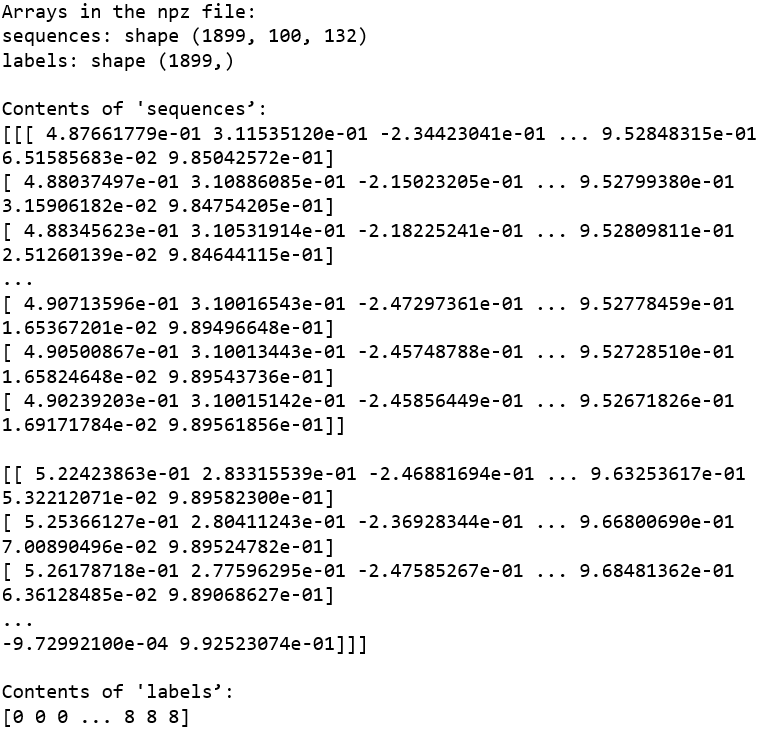
\includegraphics[width=0.8\textwidth]{bab4/ar_npzFile.png}
	\caption{The contents of the '.npz' file that stores sequences and labels data.}
	\label{fig:npzFile}
\end{figure}

To perform training, each extracted data frame is saved into a single file. Each frame generates a set of keypoints that are stored in an array. Frames from one video are collected in one time window to create a sequence. Each window is labeled according to the training activity class. The data is organized following the form of equations \ref{eq: pers.5} and \ref{eq: pers.6}. This array of data is stored in '.npz' format, a format capable of storing multiple arrays. Figure \ref{fig:npzFile} shows the contents of the '.npz' file containing the data ready for the training process.
% Untuk melakukan pelatihan, masing-masing data ekstraksi yang dimiliki kemudian disimpan ke dalam satu file. Setiap frame menghasilkan satu set keypoint yang disimpan dalam array. Frame dai satu video dikumpulkan dalam satu jendela waktu untuk membuat sequence. Masing-masing jendela diberi label sesuai dengan kelas aktifitas latihan. Data yang disusun mengikuti bentuk persamaan \ref{eq: pers.5} dan \ref{eq: pers.6}. Susunan data ini disimpan daa format '.npz', sebuah format yang mampu menyimpan multi array. Gambar \ref{fig:npzFile} menunjukkan isi dari file '.npz' yang berisikan data yang siap untuk prose pelatihan. 



\section{Performance Metrics Evaluation}
\label{sec4:evaluation}

We have trained various deep learning architectures on the PhysioExercise dataset. The tested architectures include CNN, LSTM, CNN-LSTM, and deep CNN-LSTM. From each of these architectures, we managed to develop one best model, which we then compared against each other to evaluate their performance.
% Kami telah melatih berbagai arsitektur deep learning pada dataset PhysioExercise. Arsitektur yang diuji termasuk CNN, LSTM, CNN-LSTM, dan deep CNN-LSTM. Dari setiap arsitektur ini, kami berhasil mengembangkan satu model terbaik, yang kemudian kami bandingkan satu sama lain untuk mengevaluasi kinerja mereka.

\subsection{CNN Model Performance}
\label{subsec4:CNNPerformance}

One of the architectures used in this work is the CNN architecture. This section describes the performance of the CNN model using the PhysioExercise dataset. Figure \ref{fig:CNN_AccLoss} is the accuracy and loss graph for training and validation data. This graph provides an overview of how the model behaves during the training and validation process using the CNN architecture. The training was done in 100 epochs. In the initial 20 epochs, the model experienced a fairly high increase in accuracy. The increase occurred around 0.2 to 0.6 in these first 20 epochs. After entering the 21st epoch, the training accuracy continued to increase and stabilized at around 0.8 accuracy, while the validation accuracy fluctuated between 0.7 to 0.8. This fluctuation shows that the model experienced some overfitting at some points. This overfitting indicates that the model is too adaptive to the training data and less able to generalize to the validation data.
% Salah satu arsitektur yang digunakan pada pekerjaan ini adalah arsitektur CNN. Bagian ini menjelaskan peforma dari model CNN menggunakan dataset PhysioExercise. Gambar \ref{fig:CNN_AccLoss} adalah grafik akurasi dan loss untuk data latih dan validasi. Grafik ini memberikan gambaran umum bagaimana model berperilaku selama proses pelatihan dan validasi menggunakan arsitektur CNN. Pelatihan dilakukan dalam 100 epoch. Pada 20 epoch awal, model mengalami peningkatan akurasi yang cukup tinggi. Peningkatan terjadi sekitar 0.2 menjadi 0.6 dalam 20 epoch pertama ini. Setelah memasuki epoch ke 21, akurasi pelatihan terus meningkat dan stabil pada kisaran akurasi 0.8, sedangkan akurasi validasi mengalami fluktuasi antara 0.7 hingga 0.8. Fluktuasi ini menunjukkan model mengalami beebrapa overfitting pada beberapa titik. Overfitting ini menunjukkan model terlalu menyesuaikan dengan data latih dan kurang dapat generalisasi ke data validasi.

\begin{figure}[h!]
	\centering
	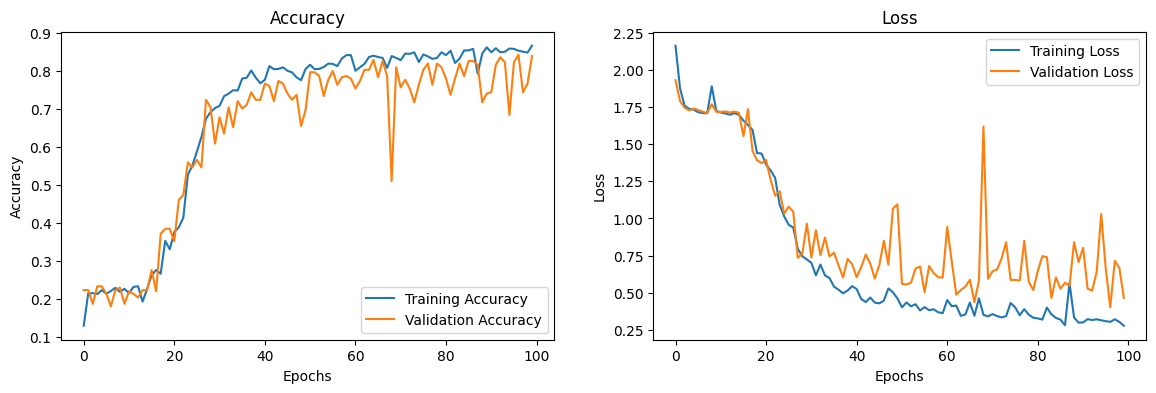
\includegraphics[width=1\textwidth]{bab4/ar_CNN_AccLoss.png}
	\caption{Accuracy and loss of training and validation on the CNN model.}
	\label{fig:CNN_AccLoss}
\end{figure}

In the first 20 epochs of the loss graph, the model loss has decreased dramatically to below 1.0. This value shows that the model is starting to be able to predict accurately. Training and validation loss tend to decrease until the end of training. However, validation loss does not decrease as well as training loss. In addition, the validation loss experiences several peaks and significant fluctuations. This graph once again shows an overfitting model and a lack of generalization to the validation data.
% Pada 20 epoch pertama dari grafik kehilangan, kehilangan model telah menurun secara dramatis hingga di bawah 1,0. Nilai ini menunjukkan model mulai mampu melakukan prediksi dengan akurat. Training dan validation loss cenderung menurun hingga akhir pelatihan. Namun, validation loss tidak menurun sebaik training loss. Selain itu, loss validasi mengalami beberapa kali puncakd an fluktuasi yang signifikan. Grafik ini sekali lagi menunjukkan model yang overfitting dan kurang mampu generalisasi ke data validasi.

\begin{figure}[h!]
	\centering
	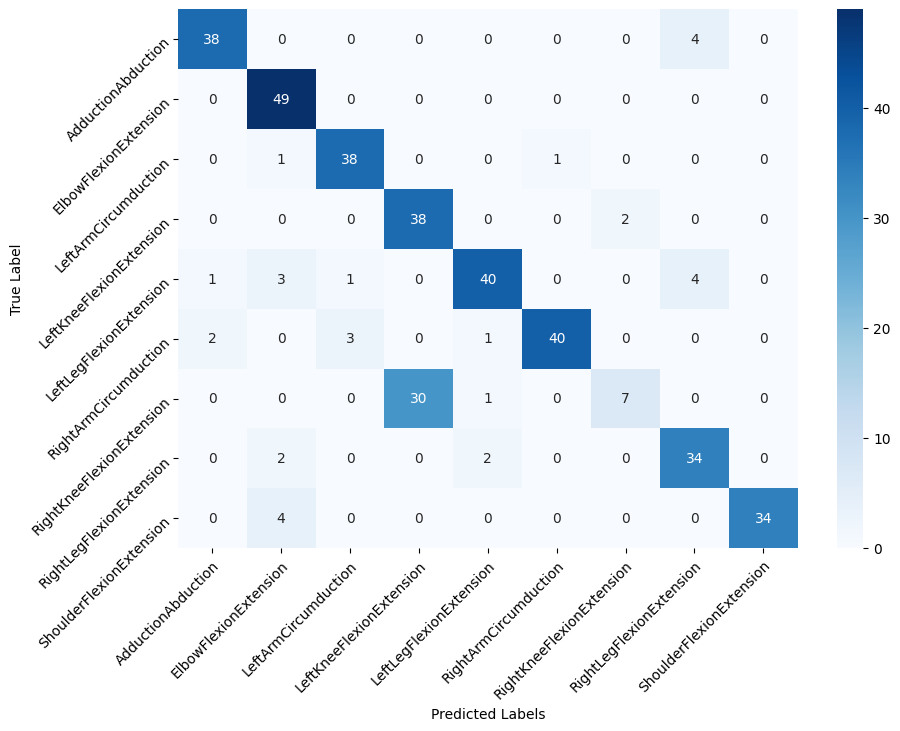
\includegraphics[width=1\textwidth]{bab4/ar_CNN_Confmatrix.png}
	\caption{Confusion matrix of the CNN model outcomes.}
	\label{fig:CNN_Confmatrix}
\end{figure}

The confusion matrix shown in figure \ref{fig:CNN_Confmatrix} provides a visual representation of the performance of the CNN model in classifying exercise activities for the elderly. Each row of the confusion matrix shows the actual number of instances for each class, while each column shows the number of instances predicted by the model for each class. There are 4 classes that show excellent performance, namely in the ElbowFlexionExtension, LeftArmCircumduction, RightArmCircumduction, and ShoulderFlexionExtension classes. The model predictions in these classes closely match the actual labels, with 49, 38, 30, and 34 correctly classified instances, respectively.
% Confusion matrix yang ditampilkan pada gambar \ref{fig:CNN_Confmatrix} memberikan gambaran visual tentang performa model CNN dalam mengklasifikasikan aktivitas latihan untuk elderly. Setiap baris dari confusion matrix menunjukkan jumlah instance aktual untuk setiap kelas, sementara setiap kolom menunjukkan jumlah instance yang diprediksi oleh model untuk setiap kelas. Terdapat 4 kelas yang menunjukkan peforma sangat baik, yaitu pada kelas ElbowFlexionExtension, LeftArmCircumduction, RightArmCircumduction, dan ShoulderFlexionExtension. Prediksi model pada kelas ini sangat sesuai dengan label sebenarnya, dengan masing-masing memiliki 49, 38, 30, dan 34 instance yang diklasifikasikan dengan benar. 

However, there are classes that experience significant confusion in making predictions. That class is RightKneeFlexionExtension. Of the 38 instances in the RightKneeFlexionExtension class, only 7 were correctly classified, while 30 instances were classified as LeftKneeFlexionExtension. These errors contributed to the low precision and recall of these classes, as shown in the classification report. This misclassification can occur based on several factors. One of the main factors is the similarity in motion between the two. The model failed to predict the RightKneeFlexionExtension instance instead classifying it as LeftKneeFlexionExtension. The similar features between the two are the main reason for the model's confusion in classifying correctly. Although the model showed good ability in classifying most of the classes, further improvement is needed to reduce confusion between classes that have movements that may be visually similar.
% Akan tetapi, terdapat kelas yang mengalami kebingungan signifikan dalam melakukan prediksi. Kelas tersebut adalah RightKneeFlexionExtension. Dari 38 instance pada kelas RightKneeFlexionExtension, hanya 7 yang diklasifikasikan dengan benar, sementara 30 instance diklasifikasikan sebagai LeftKneeFlexionExtension. Kesalahan ini berkontribusi pada rendahnya precision dan recall pada kelas-kelas tersebut, seperti yang ditunjukkan pada classification report. Kesalahan dalam klasifikasi ini dapat terjadi berdasarkan beberap faktor. Salah satu faktor utamanya adalah kemiripan gerakan diantara keduanya. Model gagal memprediksi instance RightKneeFlexionExtension alih-alih mengklasifikasikannya sebagai LeftKneeFlexionExtension. Fitur yang mirip diantara keduanya menjadi alasan utama model mengalami kebingungan dalam mengklasifikasikan dengan benar. Meskipun model menunjukkan kemampuan yang baik dalam mengklasifikasikan sebagian besar kelas, peningkatan lebih lanjut diperlukan untuk mengurangi kebingungan antar kelas yang memiliki gerakan yang mungkin secara visual mirip.

\begin{table}[h!]
	\centering
	\caption{Classification report of the CNN model.}
	\label{tab:CNNreport}
	\begin{tabular}{rrrrr}
		\multicolumn{1}{l}{}      & precision            & recall               & f1-score             & support              \\
		\multicolumn{1}{l}{}      &                      &                      &                      &                      \\
		AdductionAbduction        & 0.93                 & 0.90                 & 0.92                 & 42                   \\
		ElbowFlexionExtension     & 0.83                 & 1.00                 & 0.91                 & 49                   \\
		LeftArmCircumduction      & 0.90                 & 0.95                 & 0.93                 & 40                   \\
		LeftKneeFlexionExtension  & 0.56                 & 0.95                 & 0.70                 & 40                   \\
		LeftLegFlexionExtension   & 0.91                 & 0.82                 & 0.86                 & 49                   \\
		RightArmCircumduction     & 0.98                 & 0.87                 & 0.92                 & 46                   \\
		RightKneeFlexionExtension & 0.78                 & 0.18                 & 0.30                 & 38                   \\
		RightLegFlexionExtension  & 0.81                 & 0.89                 & 0.85                 & 38                   \\
		ShoulderFlexionExtension  & 1.00                 & 0.89                 & 0.94                 & 38                   \\
		\multicolumn{1}{l}{}      & \multicolumn{1}{l}{} & \multicolumn{1}{l}{} & \multicolumn{1}{l}{} & \multicolumn{1}{l}{} \\
		accuracy                  &                      &                      & 0.84                 & 380                  \\
		macro avg                 & 0.85                 & 0.83                 & 0.81                 & 380                  \\
		weighted avg              & 0.86                 & 0.84                 & 0.82                 & 380
	\end{tabular}%
\end{table}

Table \ref{tab:CNNreport} presents the classification report for the model using CNN architecture. Evaluation using the classification report shows the precision, recall, and f1-score metrics for each activity. This classification model has shown quite good performance. Overall, the accuracy of this model is 84\%. The overall results for each metric were calculated using macro averaging and weighted averaging methods. Using macro averaging, the average results for precision, recall, and f1-score of this model are 0.85, 0.83, and 0.81 respectively. Unlike the macro averaging method, calculations using the weighted averaging method showed a precision of 0.86, recall of 0.84, and F1-score of 0.82. This method is more representative of the class distribution in a dataset.
% Tabel \ref{tab:CNNreport} menyajikan classification report untuk model menggunakan CNN arsitektur. Evaluasi menggunakan classification report menunjukkan metris precision, recall, dan F1-score untuk setiap aktifitas. Model klasifikasi ini telah menunjukkan peforma yang cukup baik. Secara keseluruhan, akurasi model ini sebesar 84\%. Hasil keseluruhan pada setiap metrisnya dihitung menggunakan metode macro averaging dan weighted averaging. Menggunakan macro averaging, hasil rata-rata untuk precision, recall, dan F1-score model ini sebesar 0.85, 0.83, dan 0.81 respectively. Berbeda dengan metode macro averaging, perhitungan menggunakan metode weighted averaging menunjukkan hasil precision sebesar 0.86, recall sebesar 0.84, dan F1-score sebesar 0.82. Metode ini lebih representatif terhadap distribusi kelas dalam sebuah dataset.

The ShoulderFlexionExtension and RightArmCircumduction classes have very high precision, reaching 1.00 and 0.98 respectively. This value indicates that there are very few false positives in the predictions for these activities. This explanation is in line with the confusion matrix results where these classes can predict all instances well. However, the model showed difficulty with the RightKneeFlexionExtension class with a precision of only 0.78 and recall of 0.18. This indicates a large number of false negatives that affect the model's ability to detect this activity. The LeftKneeFlexionExtension activity also has a relatively low precision of 0.56 although the recall is quite high at 0.95, indicating that the model often incorrectly predicts this class as another activity.
% Kelas ShoulderFlexionExtension dan RightArmCircumduction memiliki precision yang sangat tinggi, masing-masing mencapai 1.00 dan 0.98. Nilai ini menunjukkan sedikitnya false positives pada prediksi untuk aktifitas ini. Penjelasan ini selaras dengan hasil confusion matrix di mana kelas ini dapat memprediksi seluruh instance dengan baik. Namun, model menunjukkan kesulitan pada kelas RightKneeFlexionExtension dengan precision hanya 0.78 dan recall 0.18. Nilai ini mengindikasikan banyaknya false negatives yang mempengaruhi kemampuan model dalam mendeteksi aktifitas ini. Aktifitas LeftKneeFlexionExtension juga memiliki precision yang relatif rendah sebesar 0.56 meskipun recall cukup tinggi pada 0.95, menunjukkan bahwa model sering salah dalam memprediksi kelas ini sebagai aktifitas lain.

\begin{table}[h!]
	\caption{Accuracy results for training, validation, and test data of the CNN model.}
	\label{tab:CNNAccuracy}
	\centering
	\begin{tabular}{|c|c|c|}
		\hline
		Training accuracy (\%) & Validation accuracy (\%) & Test accuracy (\%) \\ \hline
		86.83                  & 83.83                    & 83.68              \\ \hline
	\end{tabular}
\end{table}

Table \ref{tab:CNNAccuracy} is a summary of the accuracy for training, validation, and test data. Of the three, the accuracy value of the CNN model shows a consistent value. The model achieved a training accuracy of 86.83\%, which shows that the model is able to learn well from the training data. The validation accuracy of 83.83\% shows that the model has a good generalization ability to data not seen during training. Both accuracy results are consistent with the previous accuracy-loss graph where the validation accuracy remains stable around 0.83 after 20 epochs. The test accuracy value of 83.68\% confirms that the model performance remains stable when tested on an entirely new dataset. This indicates that the model did not experience significant overfitting. This is also supported by the classification report and confusion matrix which show that most classes are well classified, although there are some classes that show lower performance such as RightKneeFlexionExtension. The consistency between training, validation and test accuracies shows that the model performs reliably in this classification task, although there is still room for improvement especially in classes that show higher misclassification.
% Tabel \ref{tab:CNNAccuracy} merupakan rangkuman dari akurasi untuk data training, validasi, dan test. Dari ketiganya, nilai akurasi model CNN menunjukkan nilai yang konsisten. Model mencapai akurasi pelatihan sebesar 86.83\%, yang menunjukkan bahwa model mampu belajar dengan baik dari data pelatihan. Akurasi validasi sebesar 83.83\% menunjukkan bahwa model memiliki kemampuan generalisasi yang baik terhadap data yang tidak terlihat selama pelatihan. Kedua hasil akurasi ini konsisten dengan grafik akurasi-loss sebelumnya di mana akurasi validasi tetap stabil di sekitar 0.83 setelah 20 epoch. Nilai akurasi uji sebesar 83.68\% mengkonfirmasi bahwa performa model tetap stabil ketika diuji pada dataset yang sepenuhnya baru. Kondisi ini mengindikasikan bahwa model tidak mengalami overfitting yang signifikan. Hal ini juga didukung oleh classification report dan confusion matrix yang menunjukkan bahwa sebagian besar kelas diklasifikasikan dengan baik, meskipun terdapat beberapa kelas yang menunjukkan performa lebih rendah seperti RightKneeFlexionExtension. Konsistensi antara akurasi pelatihan, validasi, dan uji menunjukkan bahwa model memiliki performa yang andal dalam tugas klasifikasi ini, meskipun masih ada ruang untuk perbaikan terutama pada kelas-kelas yang menunjukkan kesalahan klasifikasi yang lebih tinggi.

\subsection{LSTM Model Performance}
\label{subsec4:LSTMPerformance}

\begin{figure}[h!]
	\centering
	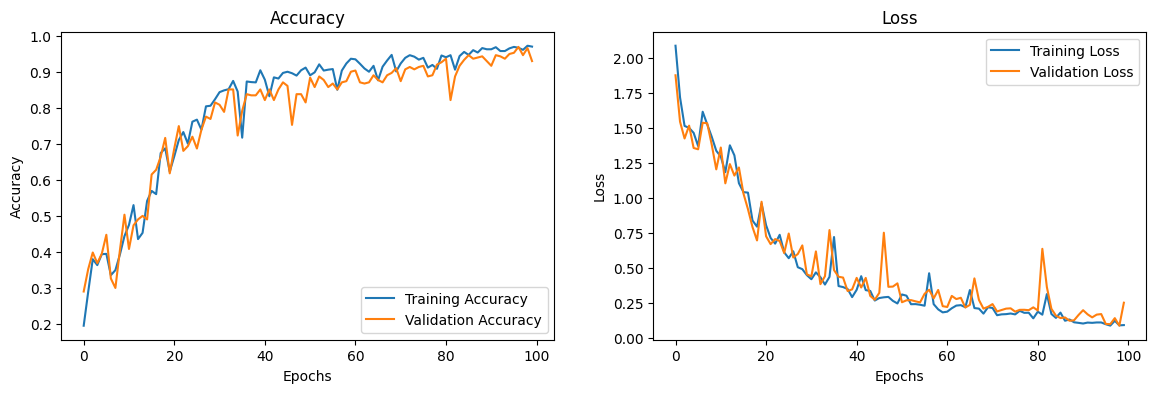
\includegraphics[width=1\textwidth]{bab4/ar_LSTM_AccLoss.png}
	\caption{Accuracy and loss of training and validation on the LSTM model.}
	\label{fig:LSTM_AccLoss}
\end{figure}

Training of the PhysioExercise dataset was also performed using the LSTM architecture. Figure \ref{fig:LSTM_AccLoss} represents the accuracy and loss graphs for training and validation data for each training epoch. The training has been done in 100 epochs. The accuracy graph on the left depicts the increase in accuracy in both the training data (Training Accuracy) and validation data (Validation Accuracy). At the beginning of training, both accuracies increase rapidly, indicating that the model immediately starts learning patterns from the data. Validation accuracy also shows an increasing trend, although there are some larger fluctuations. These fluctuations indicate a slight overfitting but overall it still generalizes well to the untrained data.
% Pelatihan dataset PhysioExercise juga dilakukan menggunakan arsitektur LSTM. Gambar \ref{fig:LSTM_AccLoss} merupakan grafik akurasi dan loss untuk data training dan validasi setiap epoch pelatihan. Pelatihan telah dilakukan dalam 100 epoch. Grafik akurasi di sebelah kiri menggambarkan peningkatan akurasi baik pada data pelatihan (Training Accuracy) maupun data validasi (Validation Accuracy). Pada awal pelatihan, kedua akurasi meningkat dengan cepat, mengindikasikan bahwa model segera mulai belajar pola dari data. Akurasi validasi juga menunjukkan tren peningkatan, meskipun terdapat beberapa fluktuasi yang lebih besar. Fluktuasi ini mengindikasikan adanya sedikit overfitting namun secara keseluruhan tetap mampu generalisasi dengan baik ke data yang tidak dilatih.

The loss graph on the right illustrates the decrease in loss in both the training data (Training Loss) and the validation data (Validation Loss). At the beginning of training, both losses decrease rapidly. The rapidly decreasing loss values indicate that the model is quickly reducing the prediction error. The training loss continues to decrease and approaches zero, indicating that the model is almost perfect on the training data. Meanwhile, the validation loss also decreases but with larger fluctuations, indicating that there are some epochs where the model does not predict the validation data as accurately as in other epochs. This fluctuation could be an indication of overfitting, where the model learns too specifically on the training data and is less able to generalize to new data. On the other hand, the validation loss value is still above the training loss value by quite a distance.
% Grafik loss di sebelah kanan menggambarkan penurunan loss baik pada data pelatihan (Training Loss) maupun data validasi (Validation Loss). Pada awal pelatihan, kedua loss menurun dengan cepat. Nilai loss yang menurun dengan cepat menunjukkan bahwa model dengan cepat mengurangi kesalahan prediksi. Loss pelatihan terus menurun dan mendekati nol, mengindikasikan bahwa model hampir sempurna pada data pelatihan. Sementara itu, loss validasi juga menurun tetapi dengan fluktuasi yang lebih besar, menunjukkan adanya beberapa epoch di mana model tidak memprediksi data validasi seakurat pada epoch lainnya. Fluktuasi ini dapat menjadi indikasi overfitting, di mana model belajar terlalu spesifik pada data pelatihan dan kurang mampu generalisasi pada data baru. Di sisi lain, nilai loss validasi masih berada di atas dari nilai loss training cukup jauh.

\begin{figure}[h!]
	\centering
	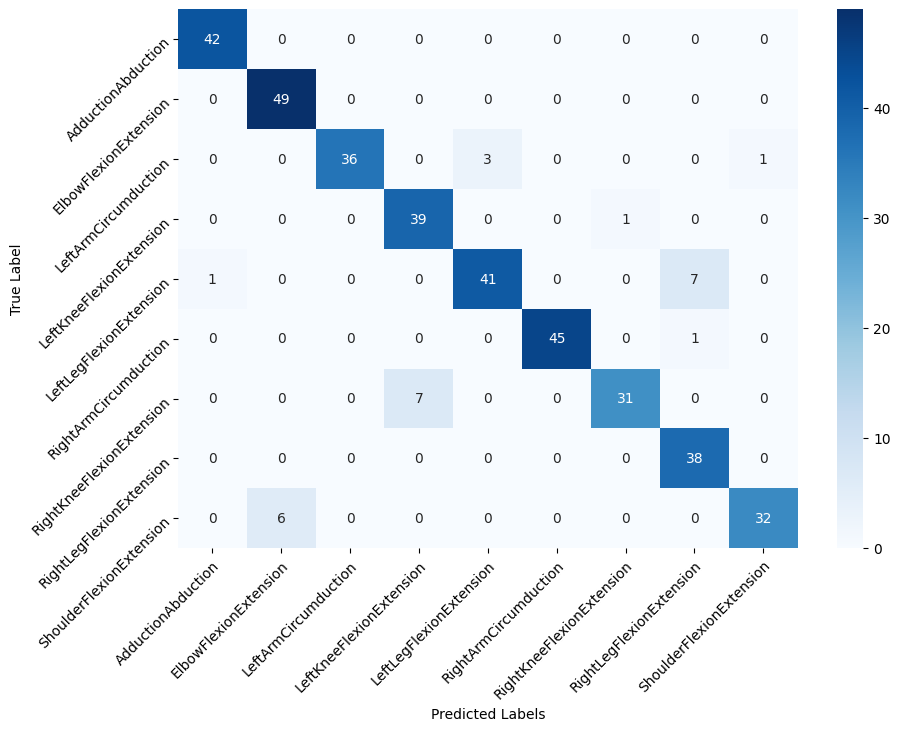
\includegraphics[width=1\textwidth]{bab4/ar_LSTM_Confmatrix.png}
	\caption{Confusion matrix of the LSTM model outcomes.}
	\label{fig:LSTM_Confmatrix}
\end{figure}

The confusion matrix of the LSTM model for classification of exercise activities in the elderly is shown in figure \ref{fig:LSTM_Confmatrix}. This confusion matrix describes the number of correct predictions (main diagonal) and misclassifications (off-diagonal) for each class. Looking at the main diagonal, it appears that the model managed to classify most of the data correctly. Some examples are in the AdductionAbduction activity with 42 correctly classified data, ElbowFlexionExtension with 49 correctly classified data, and RightLegFlexionExtension with 38 correctly classified data. However, there are some classes that experience errors in classification. For example, the LeftLegFlexionExtension class predicts 7 data as RightLegFlexionExtension, and the RightKneeFlexionExtension class predicts 6 data as LeftKneeFlexionExtension.
% Confusion matrix model LSTM untuk klasifikasi aktivitas latihan pada elderly, ditunjukkan pada gambar \ref{fig:LSTM_Confmatrix}. Confusion matrix ini menjelaskan jumlah prediksi yang benar (diagonal utama) dan kesalahan klasifikasi (off-diagonal) untuk setiap kelasnya. Melihat diagonal utama, tampak bahwa model berhasil mengklasifikasikan sebagian besar data dengan benar. Beberapa contohnya adalah pada aktifitas AdductionAbduction dengan 42 data terklasifikasi dengan benar, ElbowFlexionExtension dengan 49 data terklasifikasi dengan benar, dan RightLegFlexionExtension dengan 38 data terklasifikasi dengan benar. Akan tetapi, terdapat beberapa kelas yang mengalami kesalahan dalam klasifikasi. Sebagai contoh, kelas LeftLegFlexionExtension memprediksi 7 data sebagai RightLegFlexionExtension, dan pada kelas RightKneeFlexionExtension memprediksi 6 data sebagai LeftKneeFlexionExtension.

As a further analysis, misclassification often occurs in classes that have similar or adjacent activities in the motion space, such as LeftLegFlexionExtension and RightLegFlexionExtension. However, the model as a whole performed quite well with high accuracy in the majority of the classes, especially AdductionAbduction, ElbowFlexionExtension, and RightLegFlexionExtension. The misclassifications indicate that although the LSTM model is solid, there is room for further improvement, such as by adding more training data or tweaking the model to improve the classification ability on hard-to-distinguish classes. Thus, this confusion matrix provides deeper insight into the model's performance in classifying exercise activities in the elderly, supports the previously described analysis, and shows areas where the model can still be improved.
% Sebagai analisis lebih lanjut, kesalahan klasifikasi sering terjadi pada kelas-kelas yang memiliki aktifitas mirip atau berdekatan dalam ruang geraknya, seperti pada LeftLegFlexionExtension dan RightLegFlexionExtension. Meskipun demikian, model secara keseluruhan memiliki peforma cukup baik dengan tingkat akurasi tinggi pada mayoritas kelas, khususnya AdductionAbduction, ElbowFlexionExtension, dan RightLegFlexionExtension. Kesalahan klasifikasi yang terjadi mengindikasikan bahwa meskipun model LSTM ini solid, ada ruang untuk perbaikan lebih lanjut, seperti dengan menambah lebih banyak data pelatihan atau melakukan penyesuaian model untuk meningkatkan kemampuan klasifikasi pada kelas-kelas yang sulit dibedakan. Dengan demikian, confusion matrix ini memberikan wawasan yang lebih dalam tentang performa model dalam mengklasifikasikan aktivitas latihan pada elderly, mendukung analisis yang telah dijelaskan sebelumnya, dan menunjukkan area-area di mana model masih dapat diperbaiki.

\begin{table}[h!]
	\centering
	\caption{Classification report of the LSTM model.}
	\label{tab:LSTMreport}
	\begin{tabular}{rrrrr}
		\multicolumn{1}{l}{}      & precision            & recall               & f1-score             & support              \\
		\multicolumn{1}{l}{}      &                      &                      &                      &                      \\
		AdductionAbduction        & 0.98                 & 1.00                 & 0.99                 & 42                   \\
		ElbowFlexionExtension     & 0.89                 & 1.00                 & 0.94                 & 49                   \\
		LeftArmCircumduction      & 1.00                 & 0.90                 & 0.95                 & 40                   \\
		LeftKneeFlexionExtension  & 0.85                 & 0.97                 & 0.91                 & 40                   \\
		LeftLegFlexionExtension   & 0.93                 & 0.84                 & 0.88                 & 49                   \\
		RightArmCircumduction     & 1.00                 & 0.98                 & 0.99                 & 46                   \\
		RightKneeFlexionExtension & 0.97                 & 0.82                 & 0.89                 & 38                   \\
		RightLegFlexionExtension  & 0.83                 & 1.00                 & 0.90                 & 38                   \\
		ShoulderFlexionExtension  & 0.97                 & 0.84                 & 0.90                 & 38                   \\
		\multicolumn{1}{l}{}      & \multicolumn{1}{l}{} & \multicolumn{1}{l}{} & \multicolumn{1}{l}{} & \multicolumn{1}{l}{} \\
		accuracy                  &                      &                      & 0.93                 & 380                  \\
		macro avg                 & 0.93                 & 0.93                 & 0.93                 & 380                  \\
		weighted avg              & 0.94                 & 0.93                 & 0.93                 & 380
	\end{tabular}%
\end{table}

An explanation of the classification report of the LSTM model is shown in table \ref{tab:LSTMreport}. This table reports the precision, recall, f1-score, and support metrics for each class, as well as macro averaging and weighted averaging of the entire model. The precision value measures the correct positive predictions out of all positive predictions made by the model. A higher precision indicates the model makes fewer errors in predicting a particular class. Based on the table \ref{tab:LSTMreport}, LeftArmCircumduction and RightArmCircumduction have a precision value of 1.00. This result shows that the model is able to predict this class well, even though they are both activities with adjacent motion spaces. RightLegFlexionExtension is the class with the lowest precision among the other classes with a precision value of 0.83. Even so, this value is still considered high for prediction work. On the other hand, recall is a metric that measures the proportion of actual instances of a class that are correctly identified by the model. In this LSTM model, there are three classes with perfect recall values, i.e., AdductionAbduction, ElbowFlexionExtension, and RightLegFlexionExtension. This value indicates that the model is able to predict these classes perfectly. The lowest recall value in this LSTM model is in the RightKneeFlexionExtension class with a value of 0.82. This value is still relatively high even though the error rate is the highest compared to other classes.
% Penjelasan mengenai classification report model LSTM ditunjukkan pada tabel \ref{tab:LSTMreport}. Tabel ini menyajikan laporan metrik precision, recall, f1-score, dan support untuk setiap kelas, serta macro averaging dan weighted averaging keseluruhan model. Nilai precision mengukur prediksi positif yang benar dari keseluruhan prediksi positif yang dibuat oleh model. Precision yang semakin tinggi menunjukkan model membuat sedikit kesalahan dalam memprediksi kelas tertentu. Berdasarkan tabel \ref{tab:LSTMreport}, LeftArmCircumduction dan RightArmCircumduction memiliki nilai precision 1.00. Hasil ini menunjukkan model mampu memprediksi kelas ini dengan baik, meskipun keduanya merupakan aktifitas dengan ruang gerak berdekatan. RightLegFlexionExtension menjadi kelas dengan tingkat precision paling rendah di antara kelas-kelas lainnya dengan nilai precision sebesar 0.83. Meski begitu, nilai ini masih dianggap tinggi untuk dalam pekerjaan prediksi. Di sisi lain, recall merupakan metrik yang mengukur proporsi instance sebenarnya dari sebuah kelas yang berhasil diidentifikasi dengan benar oleh model. Pada model LSTM ini, terdapat tiga kelas dengan nilai recall sempurna, yaitu AdductionAbduction, ElbowFlexionExtension, dan RightLegFlexionExtension. Nilai ini menunjukkan model mampu memprediksi dengan sempurna atas kelas-kelas tersebut. Nilai recall terendah pada model LSTM ini berada pada kelas RightKneeFlexionExtension dengan nilai 0.82. Nilai ini masih tergolong tinggi meskipun tingkat kekeliruannya paling banyak dibandingkan dengan kelas lainnya.

F1-score gives the average harmony of precision and recall which shows the balance between these two metrics. The classes with the highest f1-score values are AdductionAbduction and RightArmCircumduction with f1-score values of 0.99. The lowest value for this metric is 0.88 for the LeftLegFlexionExtension class. This value corresponds to its lowest recall value compared to the recall of other classes. These metrics are overall modeled using macro averaging and weighted averaging methods. In the macro averaging method, the precision, recall, and f1-score metrics have the same value, which is 0.93. On the other hand, the values of the three using the weigthed averaging method have values of 0.94, 0.93, and 0.93 respectively. Weighted averaging is considered more representative of the class distribution in a dataset.
% F1-score memberikan rata-rata keharmonisan precision dan recall dimana menunjukkan keseimbangan di antara kedua metric ini. Kelas-kelas dengan nilai f1-score tertinggi berada pada kelas AdductionAbduction dan RightArmCircumduction dengan nilai f1-score sebesar 0.99. Nilai terendaha pada metric ini adalah 0.88 pada kelas LeftLegFlexionExtension. Nilai ini berhubungan dengan nilai recall-nya yang paling rendah dibandingkan dengan recall kelas lainnya. Metric-metric ini secara keseluruhan model ditunjukkan menggunakan metode macro averaging dan weighted averaging. Pada metode macro averaging, metric precision, recall, dan f1-score memiliki nilai yang sama, yaitu 0.93. Di sisi lain, nilai ketiganya menggunakan metode weigthed averaging memiliki nilai sebesar 0.94, 0.93, dan 0.93 masing-masing. Weighted averaging dianggap lebih representatif terhadap distribusi kelas dalam sebuah dataset.

\begin{table}[h!]
	\caption{Accuracy results for training, validation, and test data of the CNN model.}
	\label{tab:LSTMAccuracy}
	\centering
	\begin{tabular}{|c|c|c|}
		\hline
		Training accuracy (\%) & Validation accuracy (\%) & Test accuracy (\%) \\ \hline
		94.93                  & 93.07                    & 92.89              \\ \hline
	\end{tabular}
\end{table}

We also measured the model accuracy for each training, validation, and test data. Table \ref{tab:LSTMAccuracy} shows the accuracy value of the model for each of these data. The training accuracy reaches 94.93\% which means the model is able to learn the patterns from the training data very well. The validation accuracy reached 93.07\%. Both values are in line with the accuracy-loss graph in figure\ref{fig:LSTM_AccLoss}, where the validation accuracy is not higher than the training accuracy. The ability of the model is shown in the test accuracy, where the data given is data that has never been read by the model. The test accuracy of this model is 92.89\%. This value indicates that the generalization ability of the model is quite good.
% Kami juga mengukur tingkat akurasi model untuk setiap data latih, validasi, dan test. Tabel \ref{tab:LSTMAccuracy} menunjukkan nilai akurasi model setiap data tersebut. Akurasi pelatihan mencapai 94.93\% yang mana model mampu mempelajari pola dari data pelatihan dengan sangat baik. Adapun akurasi validasinya mencapai 93.07\%. Nilai keduanya sejalan dengan grafik akurasi-loss pada gambar\ref{fig:LSTM_AccLoss}, di mana akurasi validasi tidak lebih tinggi dibandingkan dengan akurasi pelatihannya. Kemampuan model ditunjukkan pada akurasi test, di mana data yang diberikan merupakan data yang belum pernah dibaca oleh model. Besar akurasi test model ini adalah 92.89\%. Nilai ini mengindikasikan kemampuan generalisasi model yang cukup baik. 

\subsection{CNN-LSTM Model Performance}
\label{subsec4:CNNLSTMPerformance}

\begin{figure}[h!]
	\centering
	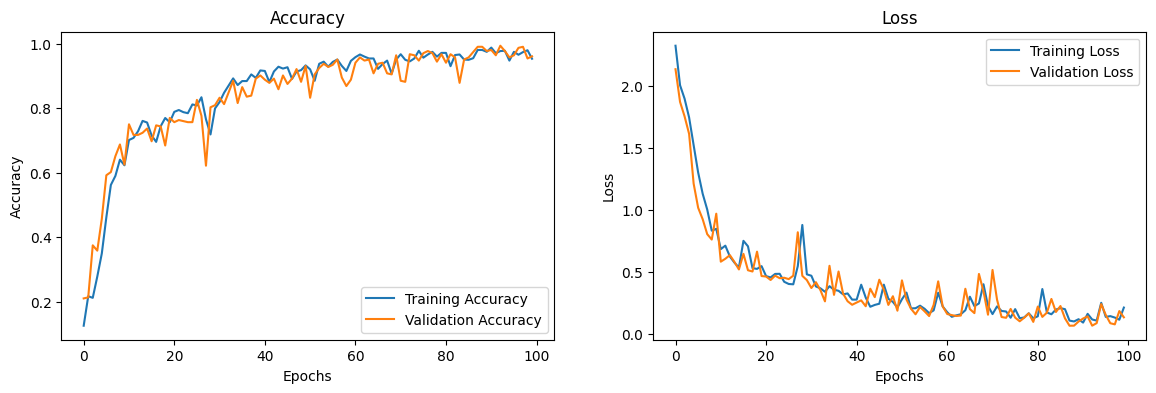
\includegraphics[width=1\textwidth]{bab4/ar_CNNLSTM_AccLoss.png}
	\caption{Accuracy and loss of training and validation on the CNN-LSTM model.}
	\label{fig:CNNLSTM_AccLoss}
\end{figure}

Another architecture used in this work is the CNN-LSTM architecture. Figure \ref{fig:CNNLSTM_AccLoss} provides an overview of the model in learning the PhysioExercise dataset. There are accuracy and loss graphs for training and validation data. The training has been done in 100 epochs. The left graph shows the accuracy of the model for each epoch. A significant improvement occurs in the first 15 epochs for training accuracy. This significant increase indicates that the model is able to learn the data patterns very well. In the following epochs, the training accuracy continues to increase until the end of the training. Although on several occasions the training accuracy had decreased, the trend in training accuracy continued to rise. Similarly, the validation accuracy experienced a significant increase for the first 15 epochs. Then the increase in accuracy occurs until the end of training although the fluctuations that occur are greater than the training accuracy. Fluctuations between training and validation accuracy occurred several times but the trend still showed an increase in accuracy until the training ended.

% Arsitektur lain yang digunakan dalam pekerjaan ini adalah arsitektur CNN-LSTM. Gambar \ref{fig:CNNLSTM_AccLoss} memberikan gambaran umum model dalam mempelajari dataset PhysioExercise. Terdapat grafik akurasi dan loss untuk data pelatihan dan validasi. Pelatihan telah dilakukan dalam 250 epoch. Grafik sebelah kiri menampilkan akurasi model setiap epochnya. Peningkatan yang cukup signifikan terjadi pada 50 epoch pertama untuk akurasi pelatihan. Peningkatan yang signifikan ini menandai model mampu mempelajari pola data dengan sangat baik. Pada epoch berikutnya, akurasi pelatihan terus mengalami kenaikan hingga akhir pelatihan. Meskipun pada beberapa kesempatan akurasi pelatihan sempat mengalami penurunan, namun tren yang terjadi pada akurasi pelatihan tetap naik. Begitu pula pada akurasi validasi, akurasi ini mengalami kenaikan yang signifikan untuk 50 epoch pertama. Kemudian kenaikan akurasi terjadi hingga akhir pelatihan meskipun fluktuasi yang terjadi lebih besar dibandingkan akurasi pelatihannya. Fluktuasi antara akurasi training maupun validasi terjadi beberapa kali namun tren masih menunjukkan kenaikan akurasi hingga pelatihan berakhir.


The loss graph shows the error rate made by the model in learning the data pattern. The loss value decreased significantly in the first 15 epochs. This graph trend applies to both training and validation losses. This decreasing loss trend continues until the end of training although fluctuations in both occur. Similar to accuracy, the loss graph fluctuates throughout the training. This fluctuation shows the ability of the model to learn the given data pattern. The validation graph has larger fluctuations when compared to the training graph. This shows the ability of the model to learn the data several times overfitting. However, the difference between the two values does not show a high number so that the model's ability to generalize data patterns is still considered good.

% Grafik loss menunjukkan tingkat kesalahan yang dilakukan oleh model dalam mempelajari pola data. Nilai loss mengalami penurunan yang cukup signifikan pada 50 epoch pertama meskipun sempat terjadi pelonjakan pada epoch ke 14. Tren grafik ini berlaku untuk loss pelatihan maupun validasi. Tren loss yang menurun ini terus berlangsung hingga akhir pelatihan meskipun fluktuasi pada keduanya terjadi. Sama halnya dengan akurasi, grafik loss ini mengalami fluktuasi disepanjang pelatihan. Fluktuasi ini menunjukkan kemampuan model dalam mempelajari pola data yang diberikan. Grafik validasi memiliki fluktuasi yang lebih besar apabila dibandingkan dengan grafik pelatihan. Hal ini menunjukkan kemampuan model dalam mepelajari data mengalami beberapa kali overfitting. Namun, perbedaan nilai keduanya tidak menunjukkan angka yang tinggi sehingga kemampuan model dalam generalisasi pola data masih dianggap baik.

\begin{figure}[h!]
	\centering
	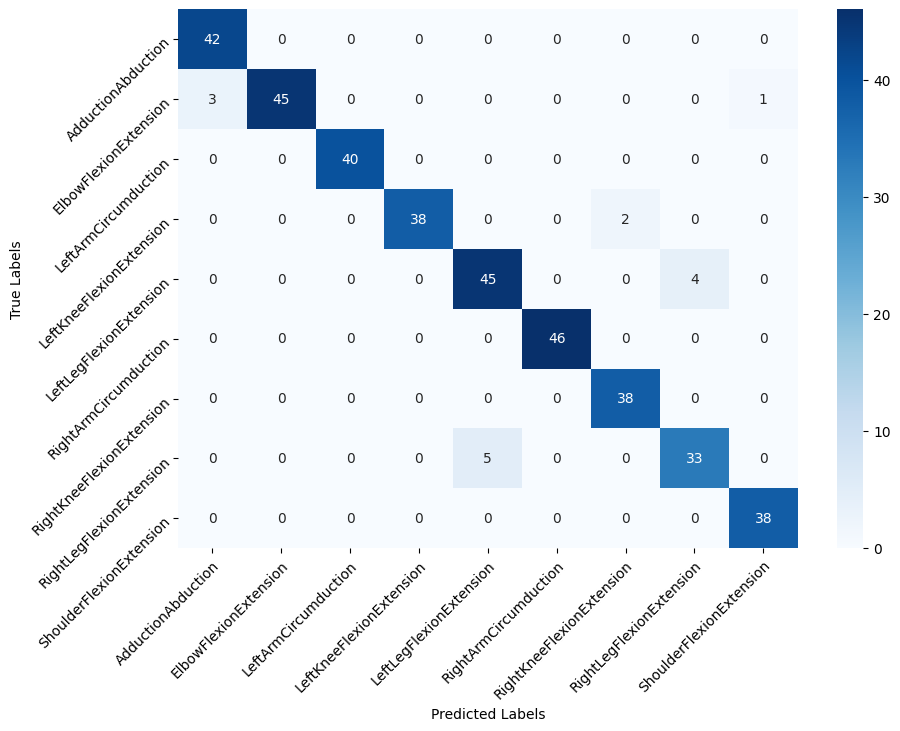
\includegraphics[width=1\textwidth]{bab4/ar_CNNLSTM_Confmatrix.png}
	\caption{Confusion matrix of the CNN-LSTM model outcomes.}
	\label{fig:CNNLSTM_Confmatrix}
\end{figure}

Figure \ref{fig:CNNLSTM_Confmatrix} displays the confusion matrix of the CNN-LSTM model. This confusion matrix illustrates the performance of the model in classifying various exercise activities for the elderly. The main diagonal shows the number of correct predictions for each class, while values off the main diagonal show the number of incorrect predictions.
% Gambar \ref{fig:CNNLSTM_Confmatrix} menampilkan confusion matrix model CNN-LSTM. Confusion matrix ini menggambarkan peforma model dalam mengklasifikasikan berbagai aktivitas latihan untuk lansia. Diagonal utama menunjukkan jumlah prediksi yang benar untuk setiap kelasnya, sementara nilai di luat diagonal utama menunjukkan jumlah prediksi yang salah.

Based on this matrix analysis, it appears that the model performs very well in classifying exercise activities for all classes. For example, the AdductionAbduction class, the model successfully predicted correctly 42 times without any errors. In addition to the AdductionAbduction class, there are other classes that were successfully predicted without any errors, i.e., LeftArmCircumduction, RightArmCircumduction, RightKneeFlexionExtension, and ShoulderFlexionExtension. The other class had some errors when the model tried to predict. For instance, 3 instances of the ElbowFlexionExtension class are considered as AdductionAbduction and 1 instance as ShoulderFlexionExtension. The RightLegFlexionExtension class has the highest error in prediction. Five instances are predicted as LeftLegFlexionExtension. Even so, this number of errors is still classified as a very low number of errors. The other class had some errors when the model tried to predict. For instance, 3 instances of the ElbowFlexionExtension class are considered as AdductionAbduction and 1 instance as ShoulderFlexionExtension. The RightLegFlexionExtension class has the highest error in prediction. Five instances are predicted as LeftLegFlexionExtension. Even so, this number of errors is still classified as a very low number of errors.
% Berdasarkan analisis matrix ini, tampak bahwa model memiliki peforma yang sangat baik dalam mengklasifikasikan aktifitas latihan untuk semua kelas. Sebagai contoh, kelas AdductionAbduction, model berhasil memprediksi dengan benar sebanyak 42 kali tanpa kesalahan. Meskipun ada beberapa kesalahan kecil, jumlah kesalahan ini tidak signifikan dan tidak mempengaruhi performa keseluruhan model secara drastis. Kesalahan prediksi ini menunjukkan bahwa model mungkin masih dapat ditingkatkan lebih lanjut, namun secara keseluruhan, model telah menunjukkan akurasi yang tinggi dan kemampuan generalisasi yang baik.

\begin{table}[h!]
	\centering
	\caption{Classification report of the CNN-LSTM model.}
	\label{tab:CNNLSTMreport}
	\begin{tabular}{rrrrr}
		\multicolumn{1}{l}{}      & precision            & recall               & f1-score             & support              \\
		\multicolumn{1}{l}{}      &                      &                      &                      &                      \\
		AdductionAbduction        & 0.93                 & 1.00                 & 0.97                 & 42                   \\
		ElbowFlexionExtension     & 1.00                 & 0.92                 & 0.96                 & 49                   \\
		LeftArmCircumduction      & 1.00                 & 1.00                 & 1.00                 & 40                   \\
		LeftKneeFlexionExtension  & 1.00                 & 0.95                 & 0.97                 & 40                   \\
		LeftLegFlexionExtension   & 0.90                 & 0.92                 & 0.91                 & 49                   \\
		RightArmCircumduction     & 1.00                 & 1.00                 & 1.00                 & 46                   \\
		RightKneeFlexionExtension & 0.95                 & 1.00                 & 0.97                 & 38                   \\
		RightLegFlexionExtension  & 0.89                 & 0.87                 & 0.88                 & 38                   \\
		ShoulderFlexionExtension  & 0.97                 & 1.00                 & 0.99                 & 38                   \\
		\multicolumn{1}{l}{}      & \multicolumn{1}{l}{} & \multicolumn{1}{l}{} & \multicolumn{1}{l}{} & \multicolumn{1}{l}{} \\
		accuracy                  &                      &                      & 0.96                 & 380                  \\
		macro avg                 & 0.96                 & 0.96                 & 0.96                 & 380                  \\
		weighted avg              & 0.96                 & 0.96                 & 0.96                 & 380
	\end{tabular}%
\end{table}

The classification report of the CNN-LSTM model is shown in table \ref{tab:CNNLSTMreport}. This table includes several metrics, i.e., precision, recall, f1-score, and support for each class. In addition, the overall value of the model is also displayed using macro averaging and weighted averaging methods. There are several classes that have perfect precision values (1.00). These classes are ElbowFlexionExtension, LeftArmCircumduction, LeftKneeFlexionExtension, and RightArmCircumduction. This value indicates that the model correctly predicted all instances of these classes. This result is in line with the explanation in the previous confusion matrix. Although not perfect, the other classes have high precision values too. The lowest precision value in this model is in the RightLegFlexionExtension class of 0.89. This value is high considering that in previous models there were several classes with lower precision values. In another metric, recall, the model is able to predict finding all positive instances very well. There are 4 classes with perfect recall values, namely AdductionAbduction, LeftArmCircumduction, RightArmCircumduction, RightKneeFlexionExtension and ShoulderFlexionExtension. Similar to precision, the lowest recall value in this model is 0.87, in the RightLegFlexionExtension and RightLegFlexionExtension classes.
% Penjelasan classification report model CNN-LSTM ditunjukkan pada tabel \ref{tab:CNNLSTMreport}. Tabel ini mencakup beberapa metris, yaitu precision, recall, f1-score, dan support untuk setiap kelasnya. Selain itu, nilai keseluruhan dari model juga ditampilkan menggunakan metode macro averaging dan weighted averaging. Terdapat beberapa kelas yang memiliki nilai precision sempurna (1.00). Kelas-kelas tersebut adalah AdductionAbduction, LeftArmCircumduction, RightKneeFlexionExtension, dan ShoulderFlexionExtension. Nilai ini menunjukkan model berhasil memprediksi dengan benar seluruh instance pada kelas tersebut. Hasil ini selaras dengan penjelasan pada confusion matrix sebelumnya. Meskipun tidak sempurna, kelas lainnya memiliki nilai precision yang tinggi juga. Nilai precision terendah pada model ini berada pada kelas RightLegFlexionExtension sebesar 0.97. Nilai ini termasuk tinggi mengingat pada model-model sebelumnya terdapat beberapa kelas dengan nilai precision lebih rendah. Pada metric yang lain, yaitu recall, model mampu memprediksi menemukan semua instance positif dengan sangat baik. Terdapat 4 kelas dengan nilai recall sempurna, yaitu AdductionAbduction, LeftArmCircumduction, LeftKneeFlexionExtension, dan ShoulderFlexionExtension. Sama halnya dengan precision, nilai recall terendah pada model ini adalah 0.97, pada kelas RightKneeFlexionExtension dan RightLegFlexionExtension.

F1-score shows the average harmony between precision and recall. Similar to the previous two metrics, the f1-score of each class in this model shows satisfactory results. The lowest value in this metric is 0.88 and is only in one class, namely RightLegFlexionExtension. There are 2 classes with perfect f1-score values, namely LeftArmCircumduction, and RightArmCircumduction. This perfect F1-score is obtained from perfect results in the precision and recall of these classes. Both macro averaging and weighted averaging, the average value of all metrics for this model is at a very high value. For all metrics, the score was 0.96 for both methods. These results show excellent performance in all classes whether or not the data distribution is taken into account.
% F1-score menunjukkan rata-rata keharmonisan antara precision dan recall. Sama halnya dengan 2 metric sebelumnya, f1-score setiap kelas pada model ini menunjukkan hasil yang memuaskan. Nilai terendah pada metric ini adalah 0.97 dan hanya berada pada satu kelas saja, yaitu RightLegFlexionExtension. Terdapat 3 kelas dengan nilai f1-score sempurna, yaitu AdductionAbduction, LeftArmCircumduction, dan ShoulderFlexionExtension. F1-score yang sempurna ini didapatkan dari hasil yang sempurna juga pada precision dan recall kelas-kelas tersebut. Baik macro averaging maupun weighted averaging, nilai rata-rata seluruh metric untuk model ini berada pada nilai yang sangat tinggi. Untuk seluruh metrics mendapatkan nilai sebesar 0.99 pada kedua metode ini. Hasil ini menunjukkan peforma yang sangat baik di semua kelas baik memperhitungkan distribusi data yang ada maupun tidak.

\begin{table}[h!]
	\caption{Accuracy results for training, validation, and test data of the CNN-LSTM model.}
	\label{tab:CNNLSTMAccuracy}
	\centering
	\begin{tabular}{|c|c|c|}
		\hline
		Training accuracy (\%) & Validation accuracy (\%) & Test accuracy (\%) \\ \hline
		96.71                  & 96.04                    & 96.05              \\ \hline
	\end{tabular}
\end{table}

Another measurement calculated is the accuracy value of the model against the training, validation, and test data. Table \ref{tab:CNNLSTMAccuracy} shows the accuracy value of each data. The training accuracy shows a high result of 96.71\%. This high accuracy shows that the model is able to learn the training data patterns very well. The learning error is very small. On the validation data, the accuracy was 96.04\%. This high value has shown that the model is not just overfitting the training data. The model was able to classify the new data very well. This training and validation accuracy value is consistent with the previous graph which shows an increase in accuracy every epoch. Model testing was performed on completely new data using test data. The test accuracy that emerged in this model was 96.05\%. The very high accuracy on all data confirms that the model is reliable and has good generalization.
% Pengukuran lain yang dihitung adalah nilai akurasi model terhadap data latih, validasi, dan uji. Tabel \ref{tab:CNNLSTMAccuracy} menunjukkan nilai akurasi setiap datanya. Akurasi pelatihan menunjukkan hasil yang tinggi, yaitu 99.67\%. Akurasi yang tinggi ini menunjukkan bahwa model mampu mempelajari pola data pelatihan dengan sangat baik. Kesalahan pembelajaran yang terjadi begitu kecil. Pada data validasi, akurasi yang muncul sebesar 98.68\%. Nilai yang tinggi ini telah menunjukkan bahwa model tidak hanya melakukan overfitting pada data pelatihan. Model mampu mengklasifikasikan data baru dengan sangat baik. Nilai akurasi pelatihan dan validasi ini konsisten dengan grafik sebelumnya yang menunjukkan peningkatan akurasi setiap epochnya. Pengujian model dilakukan pada data yang benar-benar baru menggunakan data uji. Akurasi uji yang muncul pada model ini sebesar 98.68\%. Akurasi yang sangat tinggi pada seluruh data menegaskan 	bahwa model dapat diandalkan dan memiliki generalisasi yang baik.

\subsection{Deep CNN-LSTM Model Performance}
\label{subsec4:DeepCNNLSTMPerformance}

\begin{figure}[h!]
	\centering
	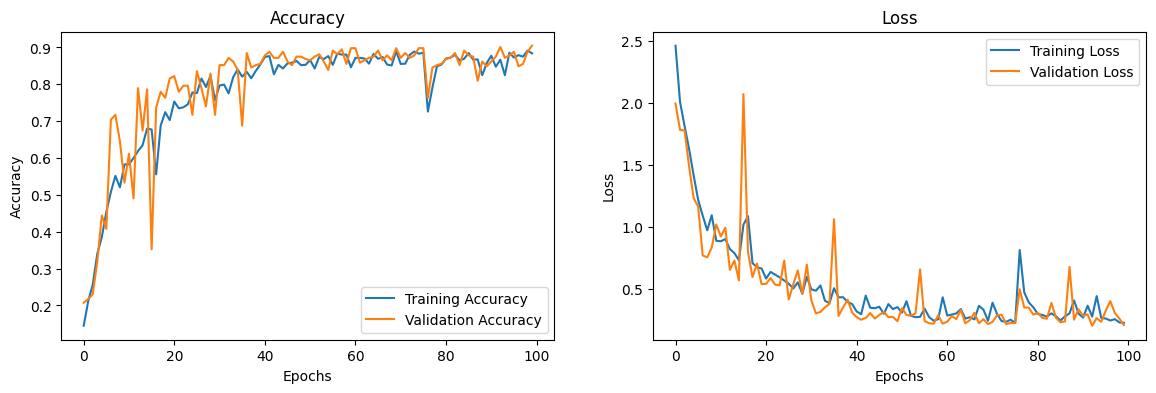
\includegraphics[width=1\textwidth]{bab4/ar_DeepCNNLSTM_AccLoss.png}
	\caption{Accuracy and loss of training and validation on the Deep CNN-LSTM model.}
	\label{fig:DeepCNNLSTM_AccLoss}
\end{figure}

The next architecture used for training the PhysioExercise dataset is deep CNN-LSTM. This training resulted in a deep CNN-LSTM model. Figure \ref{fig:DeepCNNLSTM_AccLoss} shows a detailed overview of the accuracy and loss for each epoch. There are two lines representing the training and validation data. The training took place in 100 epochs. The training accuracy of each epoch has a good increase. The gradual increase from the beginning to the end of training shows the ability of the model to learn and adapt to the given data pattern. Fluctuations occur in the training data, but the fluctuations are not too large. Unlike the validation accuracy, which experienced high fluctuations on several occasions. Even so, the trend of validation data shows the same trend as training accuracy. Both go hand in hand in improving the model's ability to learn data patterns.
% Arsitektur berikutnya yang digunakan untuk pelatihan dataset PhysioExercise adalah deep CNN-LSTM. Pelatihan ini menghasilkan sebuah model deep CNN-LSTM. Gambar \ref{fig:DeepCNNLSTM_AccLoss} menunjukkan gambaran detail akurasi dan loss setiap epochnya. Terdapat dua garis yang merepresentasikan data latih dan validasi. Pelatihan berlangsung dalam 100 epoch. Akurasi pelatihan setiap epochnya mengalami kenaikan yang baik. Kenaikan bertahap sejak awal hingga akhir pelatihan menunjukkan kemampuan model dalam mempelajari dan beradaptasi dengan pola data yang diberikan. Fluktuasi terjadi pada data pelatihan, namun fluktuasi yang terjadi tidak terlalu besar. Berbeda dengan akurasi validasi yang mengalami fluktuasi cukup tinggi dibeberapa kesempatan. Meskipun begitu, tren yang dimiliki data validasi menunjukkan tren yang sama dengan akurasi pelatihan. Keduanya beriringan dalam peningkatan kemampuan model mempelajari pola data.

The loss graph illustrates the decrease in loss values on the training and validation datasets. The decreasing value indicates that the model is able to reduce errors in learning data patterns. Entering the 41st epoch, the loss values in both training and validation experience values that tend to stabilize towards lower values. Even so, fluctuations in both losses occurred during the training process. Especially in the validation data, the loss value had a fairly high spike at some points. This spike was quite high at the beginning of the training. The spike indicates that the model had experienced some overfitting because it relied too much on the training data.
% Grafik loss menggambarkan penurunan nilai loss pada dataset pelatihan dan validasi. Nilai yang semakin menurun menunjukkan model mampu mengurangi kesalahan dalam mempelajari pola data. Loss terus mengalami penurunan hingga pada epoch ke 40. Memasuki epoch ke 41, nilai loss pada pelatihan maupun validasi mengalami nilai yang cenderung stabil menuju pada nilai yang lebih rendah. Meskipun begitu, fluktuasi pada kedua loss terjadi selama proses pelatihan berlangsung. Terutama pada data validasi, nilai loss sempat mengalami lonjakan yang cukup tinggi di beberapa titik. Lonjakan ini cukup tinggi pada awal-awal pelatihan. Kondisi lonjakan yang naik menunjukkan model sempat mengalami beberapa kali overfitting karena terlalu bertumpu pada data pelatihan. 

\begin{figure}[h!]
	\centering
	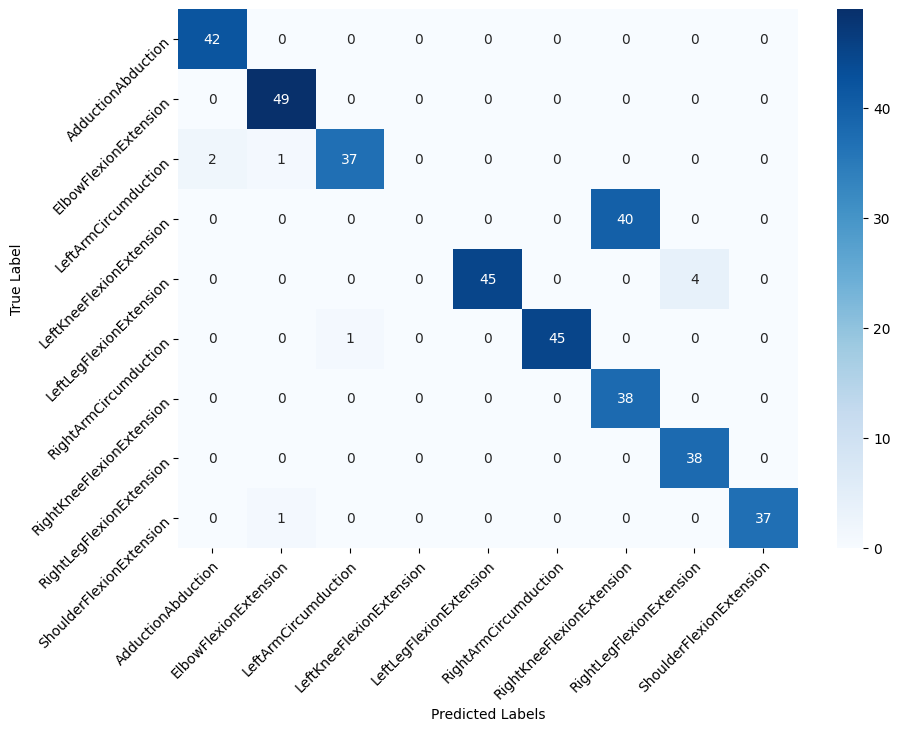
\includegraphics[width=1\textwidth]{bab4/ar_DeepCNNLSTM_Confmatrix.png}
	\caption{Confusion matrix of the Deep CNN-LSTM model outcomes.}
	\label{fig:DeepCNNLSTM_Confmatrix}
\end{figure}

Figure \ref{fig:DeepCNNLSTM_Confmatrix} displays the prediction results of the deep CNN-LSTM model against each class. The main diagonal shows the number of correct predictions for each class. While the values on the off-diagonal show the number of incorrect predictions. Overall, the model has a good ability to predict each instance. For example, the model successfully classified 42 AdductionAbduction samples, 49 ElbowFlexionExtension samples, 38 RightKneeFlexionExtension samples, and 38 RightLegFlexionExtension samples without any error.
% Gambar \ref{fig:DeepCNNLSTM_Confmatrix} menampilkan hasil prediksi model deep CNN-LSTM terhadap masing-masing kelas. Diagonal utama menunjukkan jumlah prediksi benar dari setiap kelasnya. Sedangkan nilai pada off-diagonal menunjukkan jumlah prediksi yang salah. Secara keseluruhan, model memiliki kemampuan yang baik dalam memprediksi setiap instance yang ada. Sebagai contoh, model berhasil mengklasifikasikan 42 sampel AdductionAbduction, 49 sampel ElbowFlexionExtension, 38 sampel RightKneeFlexionExtension, dan 38 sampel RightLegFlexionExtension tanpa kesalahan sama sekali. 

There was one class where the model failed to correctly predict all instances, namely the LeftKneeFlexionExtension class. Of all the instances, instead of predicting it as the LeftLegFlexionExtension class, the model predicted it as RightKneeFlexionExtension. This is a very likely error given that these two classes have similar motion spaces. In the remaining instances, the misclassification was minor and insignificant. The features of the two classes are also similar, so the model experiences confusion in classifying correctly. In addition, when looking back at the dataset, the angle of the image capture needs to be paid more attention so that the keypoint extraction process becomes better. The addition of augmentation data is important if the model is not good enough to classify all classes.
% Terdapat satu kelas dimana model gagal memprediksi dengan benar seluruh instance, yaitu kelas LeftKneeFlexionExtension. Dari seluruh instance yang ada, alih-alih memprediksi sebagai kelas LeftLegFlexionExtension, model justru memprediksi sebagai RightKneeFlexionExtension. Kesalahan sangat mungkin terjadi mengingat kedua kelas ini memiliki ruang gerak yang mirip. Fitur yang dimilki kedua kelas juga mirip, sehingga model mengalami kebingungan dalam mengklasifikasikan secara benar. Selain itu apabila melihat kembali dataset, sudut pengambilan gambar perlu lebih diperhatikan agar dalam proses ekstraksi keypoint menjadi lebih baik. Penambahan data augmentasi menjadi penting apabila model yang digunakan tidak cukup baik dalam mengklasifikasikan seluruh kelas.

The classification report of the deep CNN-LSTM model is presented in table \ref{tab:DeepCNNLSTMreport}. Evaluation using the classification report shows the precision, recall, and F1-score metrics for each activity. This classification model has shown quite good performance. Overall, the accuracy of the model was 0.87. The overall results for each metric were calculated using macro averaging and weighted averaging methods. Using macro averaging, the average results for precision, recall, and F1-score of this model are 0.81, 0.87, 0.83 respectively. Unlike the macro averaging method, calculations using the weighted averaging method showed a precision of 0.82, recall of 0.87, and F1-score of 0.84. This method is more representative of the class distribution in a dataset.
% Classification report model deep CNN-LSTM disajikan pada tabel \ref{tab:DeepCNNLSTMreport}. Evaluasi menggunakan classification report menunjukkan metris precision, recall, dan F1-score untuk setiap aktifitas. Model klasifikasi ini telah menunjukkan peforma yang cukup baik. Secara keseluruhan, akurasi model ini sebesar 87\%. Hasil keseluruhan pada setiap metrisnya dihitung menggunakan metode macro averaging dan weighted averaging. Menggunakan macro averaging, hasil rata-rata untuk precision, recall, dan F1-score model ini sebesar 0.81, 0.87, 0.83 respectively. Berbeda dengan metode macro averaging, perhitungan menggunakan metode weighted averaging menunjukkan hasil precision sebesar 0.82, recall sebesar 0.87, dan F1-score sebesar 0.84. Metode ini lebih representatif terhadap distribusi kelas dalam sebuah dataset.

\begin{table}[h!]
	\centering
	\caption{Classification report of the Deep CNN-LSTM model.}
	\label{tab:DeepCNNLSTMreport}
	\begin{tabular}{rrrrr}
		\multicolumn{1}{l}{}      & precision            & recall               & f1-score             & support              \\
		\multicolumn{1}{l}{}      &                      &                      &                      &                      \\
		AdductionAbduction        & 0.95                 & 1.00                 & 0.98                 & 42                   \\
		ElbowFlexionExtension     & 0.96                 & 1.00                 & 0.98                 & 49                   \\
		LeftArmCircumduction      & 0.97                 & 0.93                 & 0.95                 & 40                   \\
		LeftKneeFlexionExtension  & 0.00                 & 0.00                 & 0.00                 & 40                   \\
		LeftLegFlexionExtension   & 1.00                 & 0.92                 & 0.96                 & 49                   \\
		RightArmCircumduction     & 1.00                 & 0.98                 & 0.99                 & 46                   \\
		RightKneeFlexionExtension & 0.49                 & 1.00                 & 0.66                 & 38                   \\
		RightLegFlexionExtension  & 0.90                 & 1.00                 & 0.95                 & 38                   \\
		ShoulderFlexionExtension  & 1.00                 & 0.97                 & 0.99                 & 38                   \\
		\multicolumn{1}{l}{}      & \multicolumn{1}{l}{} & \multicolumn{1}{l}{} & \multicolumn{1}{l}{} & \multicolumn{1}{l}{} \\
		accuracy                  &                      &                      & 0.87                 & 380                  \\
		macro avg                 & 0.81                 & 0.87                 & 0.83                 & 380                  \\
		weighted avg              & 0.82                 & 0.87                 & 0.84                 & 380
	\end{tabular}%
\end{table}

The precision value measures the correct positive predictions out of all positive predictions made by the model. A higher precision indicates the model makes fewer errors in predicting a particular class. Based on the table \ref{tab:DeepCNNLSTMreport}, there are several classes with perfect precision values. The classes are LeftLegFlexionExtension, RightArmCircumduction, and ShoulderFlexionExtension. For the other classes, the model has a good ability to predict the given instance. However, there is one class with a very low precision value, namely RightKneeFlexionExtension. Precision in this class is only 0.49. This fairly low value indicates the number of instances that are predicted incorrectly by the model. In addition, there is one class where the model failed to predict correctly. That class is LeftKneeFlexionExtension. The precision value of 0.00 indicates that the model did not predict this class correctly at all. This precision value is in line with the discussion on the confusion matrix for the LeftKneeFlexionExtension class.
% Nilai precision mengukur prediksi positif yang benar dari keseluruhan prediksi positif yang dibuat oleh model. Precision yang semakin tinggi menunjukkan model membuat sedikit kesalahan dalam memprediksi kelas tertentu. Berdasarkan tabel \ref{tab:DeepCNNLSTMreport}, terdapat beberapa kelas dengan nilai precision sempurna. Kelas yang dimaksudkan adalah LeftLegFlexionExtension, RightArmCircumduction, dan ShoulderFlexionExtension. Terhadap kelas yang lain, model memiliki kemampuang yang baik dalam memprediksi instance yang diberikan. Namun, terdapat satu kelas dengan nilai precision sangat rendah, yaitu RightKneeFlexionExtension. Precision pada kelas ini hanya 0.49. Nilai yang cukup rendah ini menunjukkan banyaknya instance yang diprediksi salah oleh model. Selain itu, terdapat satu kelas dimana model gagal dalam memprediksi dengan benar. Kelas tersebut adalah LeftKneeFlexionExtension. Nilai precision 0.00 menujukkan model tidak sama sekali memprediksi dengan benar pada kelas ini. Nilai precision ini selaras dengan pembahasan pada confusion matrix untuk kelas LeftKneeFlexionExtension. 

Similar to precision, the recall results for some classes have perfect values. These classes are AdductionAbduction, ElbowFlexionExtension, RightKneeFlexionExtension, and RightLegFlexionExtension. This value indicates the model's good ability to find predictions for all positive instances. In the case of the RightKneeFlexionExtension class, the recall value of this class is not as bad as the precision value. Precision is quite low despite perfect recall, indicating that many predictions are wrong for this class. In the other hand, the LeftKneeFlexionExtension class gets no recall value at all, which is 0.00. In the other metric, f1-score, every class is above 0.90 except for two classes. The two classes are RightKneeFlexionExtension and LeftKneeFlexionExtension. The RightKneeFlexionExtension class had an f1-score of 0.66. This is far below the f1-score of the other classes. Even worse, the LeftKneeFlexionExtension class does not get an f1-score at all. This is related to the absence of precision and recall values for this class. The model failed to predict this class. One of the reasons is the complexity of this movement.
% Sama halnya dengan precision, hasil recall pada beberapa kelas memiliki nilai yang sempurna. Kelas-kelas tersebut adalah AdductionAbduction, ElbowFlexionExtension, RightKneeFlexionExtension, dan RightLegFlexionExtension. Nilai ini menunjukkan kemampuan baik model dalam menemukan prediksi seluruh instance positif. Pada kasus kelas RightKneeFlexionExtension, nilai recall kelas ini tidak seburuk nilai precisionnya. Precision cukup rendah meskipun recall sempurna, menunjukkan bahwa banyak prediksi yang salah untuk kelas ini. In the other hand, kelas LeftKneeFlexionExtension tidak mendapatkan nilai recall sama sekali, yaitu 0.00. Pada metric yang lain, yaitu f1-score, nilai setiap kelasnya berada di atas 0.90 kecuali dua kelas. Kedua kelas tersebut adalah RightKneeFlexionExtension dan LeftKneeFlexionExtension. Kelas RightKneeFlexionExtension mendapatkan f1-score sebesar 0.66. Nilai ini berada jauh d bawah nilai f1-score kelas lainnya. Lebih parah lagi, kelas LeftKneeFlexionExtension tidak mendapatkan nilai f1-score sama sekali. Hal ini berkaitan dengan tidak adanya nilai precision dan recall pada kelas ini. Model gagal memprediksi kelas ini. Salah satu alasannya adalah kompleksitas pada gerakan ini. 

The overall results for each metric were calculated using macro averaging and weighted averaging methods. Using macro averaging, the average results for precision, recall, and F1-score of this model are 0.81, 0.87, and 0.83 respectively. Unlike the macro averaging method, calculations using the weighted averaging method showed a precision of 0.82, recall of 0.87, and F1-score of 0.84. The macro average and weighted average of precision, recall, and F1-Score each show good values, indicating a balanced performance in most classes.
% Hasil keseluruhan pada setiap metrisnya dihitung menggunakan metode macro averaging dan weighted averaging. Menggunakan macro averaging, hasil rata-rata untuk precision, recall, dan F1-score model ini sebesar 0.81, 0.87, dan 0.83 respectively. Berbeda dengan metode macro averaging, perhitungan menggunakan metode weighted averaging menunjukkan hasil precision sebesar 0.82, recall sebesar 0.87, dan F1-score sebesar 0.84. Rata-rata makro dan rata-rata terbobot dari precision, recall, dan F1-Score masing-masing menunjukkan nilai yang baik, mengindikasikan performa yang seimbang di sebagian besar kelas. 

\begin{table}[h!]
	\caption{Accuracy results for training, validation, and test data of the deep CNN-LSTM model.}
	\label{tab:DeepCNNLSTMAccuracy}
	\centering
	\begin{tabular}{|c|c|c|}
		\hline
		Training accuracy (\%) & Validation accuracy (\%) & Test accuracy (\%) \\ \hline
		89.14                  & 90.43                    & 87.11              \\ \hline
	\end{tabular}
\end{table}

Figure \ref{tab:DeepCNNLSTMAccuracy} provides information about the accuracy of the deep CNN-LSTM model on training data, validation data, and test data. This is the final part of the evaluation series that has previously been illustrated through the accuracy and loss graphs, confusion matrix, and classification report. The model achieved an accuracy of 89.14\% on the training data. This shows that the model is able to learn from the training data quite well, identifying patterns that match the target. The accuracy on the validation data reached 90.43\%. The higher accuracy on the validation data compared to the training data indicates that the model has good generalization ability and is not overfitting on the training data. The accuracy on the test data was 87.11\%. This is the most important metric as it describes the performance of the model on data that is completely new and not seen during training and validation. This accuracy is consistent with the validation accuracy and slightly lower, which is still within reasonable limits, indicating that the model is reliable in making predictions on new data.
% Gambar \ref{tab:DeepCNNLSTMAccuracy} memberikan informasi mengenai akurasi model deep CNN-LSTM pada data latih, data validasi, dan data uji. Ini adalah bagian akhir dari rangkaian evaluasi yang sebelumnya telah diilustrasikan melalui grafik akurasi dan loss, confusion matrix, dan classification report. Model mencapai akurasi sebesar 89.14\% pada data latih. Ini menunjukkan bahwa model mampu belajar dari data pelatihan dengan cukup baik, mengidentifikasi pola yang sesuai dengan target. Akurasi pada data validasi mencapai 90.43\%. Akurasi yang lebih tinggi pada data validasi dibandingkan dengan data latih menunjukkan bahwa model memiliki kemampuan generalisasi yang baik dan tidak overfitting pada data pelatihan. Akurasi pada data uji adalah 87.11\%. Ini adalah metrik yang paling penting karena menggambarkan kinerja model pada data yang benar-benar baru dan tidak terlihat selama pelatihan dan validasi. Akurasi ini konsisten dengan akurasi validasi dan sedikit lebih rendah, yang masih dalam batas wajar, menunjukkan bahwa model dapat diandalkan dalam membuat prediksi pada data baru.


\section{Performance Analysis of Models}
\label{sec:ModelAnalysis}

There are 4 different models that have been generated in this work. These models have different architectures used. An in-depth discussion has been done in the previous section. The results of the four models were then analyzed to compare the performance of each model. Table \ref{tab:ComparisonTable} shows an overview of the performance of each model. Several metrics are taken for comparison. These metrics are precision, recall, f1-score, accuracy, and model loss.
% Terdapat 4 model berbeda yang telah dihasilkan pada pekerjaan ini. Model-model ini memiliki berbedaan arsitektur yang digunakan. Pembahasan mendalam telah dilakukan pada bagian sebelumnya. Hasil dari keempatnya kemudian dianalisis untuk dibandingkan peforma masing-masing model. Tabel \ref{tab:ComparisonTable} menunjukkan overview dari peforma setiap modelnya. Beberapa metric diambil untuk dibandingkan. Metric-metric tersebut adalah precision, recall, f1-score, accuracy, dan loss model.

\begin{table}[h!]
	\caption{Classification performance of exercise activities for the elderly on models.}
	\label{tab:ComparisonTable}
	\centering
	\begin{tabular}{|cl|r|r|r|r|}
		\hline
		\multicolumn{2}{|c|}{Metrics}                                                                     & \multicolumn{1}{c|}{CNN} & \multicolumn{1}{c|}{LSTM} & \multicolumn{1}{c|}{CNN-LSTM} & \multicolumn{1}{c|}{\begin{tabular}[c]{@{}c@{}}Deep \\ CNN-LSTM\end{tabular}}        \\ \hline
		\multicolumn{1}{|c|}{\multirow{3}{*}{\begin{tabular}[c]{@{}c@{}}Macro\\ Average\end{tabular}}}    & Precision                & 0.85                      & 0.93                          & \textbf{0.96}                                                                 & 0.81 \\ \cline{2-6}
		\multicolumn{1}{|c|}{}                                                                            & Recall                   & 0.83                      & 0.93                          & \textbf{0.96}                                                                 & 0.87 \\ \cline{2-6}
		\multicolumn{1}{|c|}{}                                                                            & F1-Score                 & 0.81                      & 0.93                          & \textbf{0.96}                                                                 & 0.83 \\ \hline
		\multicolumn{1}{|c|}{\multirow{3}{*}{\begin{tabular}[c]{@{}c@{}}Weighted\\ Average\end{tabular}}} & Precision                & 0.86                      & 0.94                          & \textbf{0.96}                                                                 & 0.82 \\ \cline{2-6}
		\multicolumn{1}{|c|}{}                                                                            & Recall                   & 0.84                      & 0.93                          & \textbf{0.96}                                                                 & 0.87 \\ \cline{2-6}
		\multicolumn{1}{|c|}{}                                                                            & F1-Score                 & 0.82                      & 0.93                          & \textbf{0.96}                                                                 & 0.84 \\ \hline
		\multicolumn{2}{|l|}{Accuracy (\%)}                                                               & 83.68                    & 92.89                     & \textbf{96.05}                & 87.11                                                                                \\ \hline
		\multicolumn{2}{|l|}{Loss}                                                                        & 0.4513                   & 0.2629                    & \textbf{0.1498}               & 0.3004                                                                               \\ \hline
	\end{tabular}
	\caption*{Higher is better. For loss, lower is better.}
\end{table}

The model performance comparison table shows that the CNN-LSTM architecture consistently has the best performance in the classification of exercise activities for the elderly compared to the CNN, LSTM, and Deep CNN-LSTM models. The CNN model is the model with the lowest performance. The accuracy value of this model is only 83.68\% and the loss value is quite high, which is 0.4513. The Deep CNN-LSTM model is the next low-performing model. The accuracy of this model is at 87.11\% with a loss value of 0.3004. Unlike the two previous models, the LSTM model has a better performance. The accuracy of this model is at a value of 92.89\% and the loss is 0.2629. The CNN-LSTM model is the model with the best performance. The accuracy of the CNN-LSTM model is 96.05\% and the loss is 0.1498. This figure shows the ability of the CNN-LSTM model in the classification work of the best exercise activity compared to other models.
% Tabel perbandingan performa model menunjukkan bahwa arsitektur CNN-LSTM secara konsisten memiliki performa terbaik dalam klasifikasi aktivitas latihan untuk elderly dibandingkan dengan model CNN, LSTM, dan Deep CNN-LSTM. Model CNN menjadi model dengan peforma paling rendah. Nilai akurasi model ini hanya 83.68% dan nilai loss yang cukup tinggi, yaitu 0.4513. Model Deep CNN-LSTM menjadi model dengan peforma rendah berikutnya. Akurasi model ini berada pada nilai 87.11% dengan loss bernilai 0.3004. Berbeda dengan kedua model sebelumnya, model LSTM memiliki peforma yang lebih baik. Akurasi model ini berada pada nilai 92.89% dan loss bernilai 0.2629. Model CNN-LSTM menjadi model dengan peforma paling baik. Akurasi model CNN-LSTM bernilai 96.05% dan loss 0.1498. Angka ini menunjukkan kemampuan model CNN-LSTM dalam pekerjaan klasifikasi aktifitas latihan paling baik dibandingkan model lainnya.

% bagian CNN
The CNN model is the model with the worst performance compared to other models. The accuracy of this model is only 83.68\%. This figure shows that the accuracy of the model in classifying exercise activities is very low. In the classification process, the CNN model has the highest error rate among other models. This is indicated by the highest loss value of the CNN model compared to other models. CNN model loss is 0.4513. There are many factors that can affect the low performance of the CNN model. CNN is a well-known architecture in the context of image data processing. In time series data processing, the time series data structure will be considered as a one-dimensional image. This data structure will consider time as one dimension and other features as other dimensions. However, CNN's ability to handle this data has many limitations. CNNs tend to be less effective in capturing long-term dependencies in time series data, especially when compared to LSTM. In addition, determining the right CNN architecture for time series is a job in itself because it is more complicated when compared to other architectures such as LSTM. The dataset used in this work is a time series data with a large number of windows and features. With the large amount of temporal and spatial data used, the CNN model did not succeed in classifying the instances properly.
% Model CNN menjadi model dengan peforma paling buruk dibandingkan dengan model lainnya. Akurasi model ini hanya bernilai 83.68\%. Angka ini menunjukkan tingkat ketepatan model dalam mengklasifikasikan aktifitas latihan sangat rendah. Dalam proses klasifikasi, model CNN memiliki tingkat kesalahan paling tinggi diantara model lainnya. Hal ini ditunjukkan dengan nilai loss model CNN tertinggi dibandingkan dengan model lainnya. Loss model CNN bernilai 0.4513. Terdapat banyak faktor yang dapat mempengaruhi peforma model CNN yang rendah ini. CNN merupakan arsitektur yang dikenal dalam konteks pengolahan data citra. Dalam pengolahan data time series, struktur data time series akan dianggap sebagai citra satu dimensi. Struktur data ini akan menganggap waktu sebagai satu dimensi dan fitur lainnya sebagai dimensi lainnya. Akan tetapi, kemampuan CNN dalam menangani data ini memiliki banyak batasan. CNN cenderung kurang efektif dalam menangkap dependensi jangka panjang dalam data time series, terutama apabila dibandingkan dengan LSTM. Selain itu, penentuan arsitektur CNN yang tepat untuk time series menjadi pekerjaan tersendiri karena lebih rumit apabila dibandingkan dengan arsitektur lainnya seperti LSTM. Dataset yang digunakan pada pekerjaan ini merupakan data time series dengan jumlah window dan fitur yang cukup banyak. Dengan banyaknya data temporal dan spasial yang digunakan, model CNN tidak berhasil melakukan klasifikasi instance dengan baik.

% bagian LSTM
The performance of the LSTM model is high compared to the CNN and Deep CNN-LSTM models. The LSTM model used in the classification of exercise activities in the elderly showed excellent performance, with high accuracy on training, validation, and test data. The accuracy-loss graph shows a steady and consistent upward trend, while the confusion matrix and classification report provide further evidence of the model's ability to correctly classify most classes. However, the model is not better when compared to the CNN-LSTM model. LSTM models are designed to capture long-term temporal dependencies, but are not effective in extracting locally or spatially significant features in short time windows. In the dataset used, the spatial data in question is the keypoint extracted features from the Mediapipe framework. The LSTM model is not able to handle this keypoint extraction data compared to the CNN-LSTM model. The LSTM model is a complex model with many parameters that can cause overfiting problems. In addition, the LSTM model requires a lot of data for effective training. In contrast to the CNN-LSTM model, where CNN will reduce the dimensions of the input entering the LSTM. In the end, the complexity of the CNN-LSTM model becomes lower and is able to improve generalization.
% Peforma model LSTM tergolong tinggi dibandingkan dengan model CNN dan Deep CNN-LSTM. Model LSTM yang digunakan dalam klasifikasi aktivitas latihan pada elderly menunjukkan performa yang sangat baik, dengan akurasi tinggi pada data pelatihan, validasi, dan uji. Grafik akurasi-loss menunjukkan tren peningkatan yang stabil dan konsisten, sementara confusion matrix dan classification report memberikan bukti lebih lanjut tentang kemampuan model dalam mengklasifikasikan sebagian besar kelas dengan benar. Meskipun begitu, model ini tidak lebih baik apabila dibandingkan dengan model CNN-LSTM. Model LSTM dirancang untuk menangkap dependensi temporal jangka panjang, namun tidak efektif dalam mengekstraksi fitur lokal atau spasial yang signifikan dalam jendela waktu yang pendek. Pada dataset yang digunakan, data spasial yang dimaksud adalah fitur ekstraksi keypoint dari framework Mediapipe. Model LSTM tidak mampu menangani data ekstraksi keypoint ini dibandingkan dengan model CNN-LSTM. Model LSTM merupakan model yang kompleks dengan banyaknya parameter yang dapat menyebabkan masalah overfiting. Selain itu, model LSTM memerlukan banyak data untuk pelatihan yang efektif. Berbeda dengan model CNN-LSTM, dimana CNN akan mereduksi dimensi input yang masuk ke LSTM. Pada akhirnya kompleksitas model CNN-LSTM menjadi lebih rendah dan mampu meningkatkan generalisasi.

% tambahan bagian LSTM
% LSTM cenderung lebih lambat dalam pelatihan dan inferensi dibandingkan CNN karena sifat sekuensialnya yang sulit untuk diparalelkan. CNN berperan dalam mereduksi dimensi, dimana inferensi menjadi lebih cepat. LSTM mungkin tidak sepenuhnya memanfaatkan struktur data 2D atau 3D yang ada dalam data keypoint, karena lebih berfokus pada urutan temporal. CNN membantu dalam ekstraksi di awal, sehingga mengurangi kebutuhan akan jumlah parameter yang besar dalam LSTM. 

% bagian CNN-LSTM
CNN-LSTM achieved the highest precision, recall, and f1-score values in both macro average and weighted average metrics, with 0.96 each. This shows that the CNN-LSTM model is highly accurate in making positive predictions and is able to detect almost all positive instances correctly, providing an optimal balance between precision and recall. In addition, the CNN-LSTM model also showed the highest accuracy of 96.05\% and the lowest loss value of 0.1498, reflecting a very low prediction error rate. The combination of CNN and LSTM shows a good ability to handle spatial data and temporal data in one dataset.
% CNN-LSTM mencapai nilai precision, recall, dan f1-score tertinggi baik dalam metrik macro average maupun weighted average, dengan masing-masing sebesar 0.99. Hal ini menunjukkan bahwa model CNN-LSTM sangat akurat dalam membuat prediksi positif dan mampu mendeteksi hampir semua instance positif dengan benar, memberikan keseimbangan yang optimal antara precision dan recall. Selain itu, model CNN-LSTM juga menunjukkan akurasi tertinggi sebesar 98.68\% dan nilai loss terendah sebesar 0.0683, yang mencerminkan tingkat kesalahan prediksi yang sangat rendah. Kombinasi CNN dan LSTM menunjukkan kemampuan yang baik dalam menangani data spasial dan data temporal dalam satu dataset. 

% bagian Deep CNN-LSTM
The Deep CNN-LSTM model is a model with poor performance after the CNN model. This model has a similar architecture to the CNN-LSTM model. The difference of this model is the addition of several CNN layers that become deeper in the training process. However, the additional layer architecture does not show better results. There are several reasons why this might happen. First, too many layers make the model learn too much from the training data and fail to generalize to the test data. This is evidenced in the figure \ref{fig:DeepCNNLSTM_AccLoss} where the accuracy of the validation dta experiences many times large fluctuations. Secondly, more complex models require more data to train effectively. If the available data is not large enough or diverse enough, adding layers is ineffective because it does not have enough information to learn the data patterns. This will create a model that needs to be. Thirdly, the addition of these layers causes redundancy in the extracted features. Instead of making the model get new information, the length of the layer adds complexity without increasing the model's ability because the information carried is the same or does not increase. This is evidenced in the figure \ref{fig:DeepCNNLSTM_Confmatrix} where there is a class that fails to be classified correctly for all its instances.
% Model Deep CNN-LSTM menjadi model dengan peforma yang buruk setelah model CNN. Model ini memiliki arsitektur yang mirip dengan model CNN-LSTM. Perbedaan dari model ini adalah penambahan beberapa layer CNN yang menjadi lebih mendalam dalam proses pelatihannya. Meskipun begitu, penambahan layer arsitektur tidak menunjukkan hasil yang lebih baik. Terdapat beberapa alasan mengapa hal ini bisa terjadi. Pertama, terlalu banyaknya jumlah layer membuat model terlalu banyak belajar dari data latih dan gagal menggeneralisasi pada data uji. Hal ini dibuktikan pada gambar \ref{fig:DeepCNNLSTM_AccLoss} dimana akurasi dta validasi mengalami berkali-kali fluktuasi yang besar. Kedua, model yang lebih kompleks membutuhkan lebih banyak data untuk dilatih secara efektif. Apabila data yang tersedia tidak cukup banyak atau tidak cukup beragam, penambahan layer menjadi tidak efektif karen tidak memiliki cukup informasi dalam mempelajari pola data. Kondisi ini akan membuat model yang butuh. Ketiga, penambahan layer ini menyebabkan deddundansi dalam ftur yang diekstraksi. Alih-alih membuat model mendapatkan informasi yang baru, panjangnya layer justru menambah kompleksitas tanpa meningkatkan kemampuan model karena informasi yang dibawa sama atau tidak bertambah. Hal ini dibuktikan pada gambar \ref{fig:DeepCNNLSTM_Confmatrix} di mana terdapat sebuah kelas yang gagal diklasifikasikan dengan benar untuk seluruh instance-nya. 

These results indicate that the combination of CNN and LSTM in the CNN-LSTM architecture provides significant advantages in this classification task. Therefore, CNN-LSTM can be considered as the most efficient and effective model for classifying exercise activities for the elderly, with potential for real applications that require accurate and reliable predictions. Meanwhile, the performance of Deep CNN-LSTM shows potential for further improvement to increase accuracy and reduce loss values.
% Hasil ini mengindikasikan bahwa kombinasi dari CNN dan LSTM dalam arsitektur CNN-LSTM memberikan keunggulan signifikan dalam tugas klasifikasi ini. Oleh karena itu, CNN-LSTM dapat dianggap sebagai model yang paling efisien dan efektif untuk mengklasifikasikan aktivitas latihan bagi elderly, dengan potensi untuk aplikasi nyata yang membutuhkan prediksi yang akurat dan andal. Sementara itu, performa Deep CNN-LSTM menunjukkan adanya potensi untuk perbaikan lebih lanjut guna meningkatkan akurasi dan mengurangi nilai loss.

\section{Processing Time Speed Result}
\label{sec4:InferenceTime}

This section describes the processing time speed of the model in classifying an instance. The experiment is conducted by randomly selecting one Inference on data that the model has never recognized before. The input for this test is video data. This data is then extracted into 100 frames following the trained model. The result of these frames is extracted keypoints and then stored into an array. The result of the data that is ready to be classified by this model is calculated processing time until it comes out the class that has been classified by the model.

\begin{table}[h!]
	\caption{Inference time of exercise activities for the elderly on models.}
	\label{tab:InferenceTime}
	\centering
	\begin{tabular}{|l|r|r|}
		\hline
		Model         & \multicolumn{1}{l|}{Inference Time (s)} & \multicolumn{1}{l|}{Percentage (\%)} \\ \hline
		CNN           & \textbf{0.1316}                         & 14.57                                \\ \hline
		LSTM          & 0.2491                                  & 27.58                                \\ \hline
		CNN-LSTM      & 0.2416                                  & 26.75                                \\ \hline
		Deep CNN-LSTM & 0.2810                                  & 31.11                                \\ \hline
	\end{tabular}
\end{table}

The CNN model shows the fastest processing time speed compared to other models. This is influenced by the simplicity of the model and the CNN model's ability to process local or spatial data. Even so, keep in mind that the CNN model has the lowest accuracy rate compared to other models. The LSTM model is not faster than the CNN-LSTM and CNN models. This can be explained because the parameter complexity of the LSTM model and its ability to handle spatial data is not better than the CNN architecture. Therefore, the CNN-LSTM model is the fastest model after the CNN model. The process in CNN reduces the dimension of the LSTM input, making the classification process slightly faster than the LSTM model alone. The Deep CNN-LSTM model is a fairly long model because of its longer and heavier process.
% Bagian ini menjelaskan kecepatan waktu pemrosesan model dalam melakukan klasifikasi sebuah instance. Percobaan dilakukan dengan memilih satu Inference secara acak pada data yang belum pernah dikenali model sebelumnya. Masukan pada pengujian ini adalah data video. Data ini kemudian diekstrak menjadi 100 frame mengikuti model yang telah dilatih. Hasil dari frame-frame ini diekstrak keypointnya lalu disimpan ke dalam sebuah array. Hasil dari data yang siap diklasifikasikan model ini dihitung waktu pemrosesannya hingga keluar kelas yang telah diklasifikasi model. Model CNN menunjukkan kecepatan waktu pemrosesan paling cepat dibandingkan dengan model lainnya. Hal ini dipengaruhi oleh model yang sederhana dan kemampuan model CNN dalam mengolah data lokal atau spasial. Meskipun begitu, perlu diingat bahwa model CNN memiliki tingkat akurasi paling rendah dibandingkan dengan model lainnya. Model LSTM tidak lebih cepat dibandingkan dengan model CNN-LSTM dan CNN. Hal ini dapat dijelaskan karena kompleksitas parameter model LSTM dan kemampuan dalam menangani data spasial tidak lebih baik dibandingkan arsitektur CNN. Oleh karena itu, model CNN-LSTM menjadi model paling cepat setelah mdoel CNN. Proses pada CNN mereduksi dimensi input LSTM sehingga membuat proses klasifikasi sedikit lebih cepat dibandingkan dengan model LSTM saja. Adapun model Deep CNN-LSTM menjadi model yang cukup lama karena prosesnya yang lebih panjang dan berat. 

% CNN
% Secara keseluruhan, hasil dari confusion matrix konsisten dengan grafik akurasi-loss dan classification report, menyoroti kekuatan model dalam mengklasifikasikan mayoritas kelas dengan baik, tetapi juga mengidentifikasi area yang memerlukan perbaikan lebih lanjut. Teknik tambahan seperti augmentasi data, penyesuaian hiperparameter, atau penggunaan model yang lebih kompleks dapat membantu meningkatkan akurasi prediksi dan mengurangi kesalahan klasifikasi pada kelas yang sulit.


% LSTM Model
% Hasil ini menunjukkan bahwa model LSTM ini efektif untuk tugas klasifikasi aktivitas latihan pada elderly, dan dengan beberapa perbaikan seperti penambahan data pelatihan atau teknik regularisasi lebih lanjut, performa model ini dapat ditingkatkan lebih jauh. Analisis komprehensif ini memberikan dasar yang kuat untuk membangun narasi dalam paper ilmiah mengenai efektivitas dan potensi perbaikan model LSTM untuk aplikasi serupa di masa depan.


% CNN-LSTM Model
% Nilai akurasi data latih, validasi, dan uji yang tinggi menunjukkan bahwa model CNN-LSTM yang telah dibangun memiliki kinerja yang sangat baik dalam klasifikasi aktivitas latihan untuk lansia. Akurasi pelatihan yang tinggi menunjukkan bahwa model berhasil belajar dengan baik dari data pelatihan. Akurasi validasi yang tinggi menunjukkan bahwa model mampu menggeneralisasi dengan baik pada data yang tidak terlihat selama pelatihan, dan akurasi uji yang tinggi menunjukkan performa yang konsisten dan dapat diandalkan pada data baru. Hasil ini konsisten dengan grafik akurasi dan loss, confusion matrix, dan classification report yang telah dibahas sebelumnya, menunjukkan bahwa model ini sangat efektif dan efisien dalam tugas klasifikasi tersebut. Penjelasan ini memberikan bukti tambahan untuk mendukung analisis dan diskusi dalam paper ilmiah yang sedang Anda tulis.

% Deep CNN-LSTM Model
% Hasil akurasi ini konsisten dengan temuan sebelumnya dari grafik akurasi dan loss, confusion matrix, dan classification report. Model deep CNN-LSTM menunjukkan performa yang kuat dengan akurasi tinggi pada ketiga set data: pelatihan, validasi, dan uji. Akurasi yang tinggi pada data validasi dan uji menunjukkan bahwa model memiliki kemampuan generalisasi yang baik, mampu mengklasifikasikan aktivitas latihan dengan baik pada data baru. Akurasi yang sedikit lebih rendah pada data uji dibandingkan dengan data latih dan validasi masih dalam batas wajar, yang mengindikasikan bahwa model tidak overfitting dan memiliki kinerja yang stabil. Ini menegaskan bahwa model deep CNN-LSTM ini efektif dan andal untuk aplikasi klasifikasi aktivitas latihan bagi lansia.




% \begin{table}[]
% 	\centering
% 	\caption{Physiotherapy exercises used as dataset classes and the distribution of each class's number.}
% 	\label{tab:class-dataset}
% 	\begin{tabular}{|l|l|l|l|}
% 		\hline
% 		\multicolumn{1}{|l|}{\textbf{Physical Issue}}      & \textbf{Physiotherapy Exercise} & \textbf{Total Person}  & \textbf{Total Video}     \\ \hline
% 		\multirow{4}{*}{Frozen Shoulder}                   & Adduction Abduction             & \multicolumn{1}{r|}{5} & \multicolumn{1}{r|}{206} \\ \cline{2-4}
% 		                                                   & Left Arm Circumduction          & \multicolumn{1}{r|}{5} & \multicolumn{1}{r|}{227} \\ \cline{2-4}
% 		                                                   & Right Arm Circumduction         & \multicolumn{1}{r|}{6} & \multicolumn{1}{r|}{227} \\ \cline{2-4}
% 		                                                   & Shoulder Flexion Tension        & \multicolumn{1}{r|}{7} & \multicolumn{1}{r|}{229} \\ \hline
% 		Tennis Elbow                                       & Elbow flexion tension           & \multicolumn{1}{r|}{5} & \multicolumn{1}{r|}{219} \\ \hline
% 		\multirow{4}{*}{Knee Pain}                         & Left Knee Flexion Extension     & \multicolumn{1}{r|}{5} & \multicolumn{1}{r|}{195} \\ \cline{2-4}
% 		                                                   & Right Knee Flexion Extension    & \multicolumn{1}{r|}{5} & \multicolumn{1}{r|}{195} \\ \cline{2-4}
% 		                                                   & Left Leg Flexion Extension      & \multicolumn{1}{r|}{5} & \multicolumn{1}{r|}{206} \\ \cline{2-4}
% 		                                                   & Right Leg Flexion Extension     & \multicolumn{1}{r|}{5} & \multicolumn{1}{r|}{195} \\ \hline
% 		\multicolumn{3}{|l|}{\textbf{Total video dataset}} & \multicolumn{1}{r|}{1899}                                                           \\ \hline
% 	\end{tabular}
% \end{table}

% \begin{table}[h!]
% 	\caption{Physiotherapy exercises used as dataset classes and the distribution of each class's number.}
% 	\label{tab:class-dataset}
% 	\centering
% 	\begin{tabularx}{\textwidth}{|l|X|r|r|}
% 		\hline
% 		\textbf{Physical Issue}                            & \textbf{Physiotherapy \newline Exercise} & \textbf{Total Person} & \textbf{Total Video} \\ \hline
% 		\multirow{4}{*}{Frozen Shoulder}
% 		                                                   & Adduction \newline Abduction             & 5                     & 206                  \\ \cline{2-4}
% 		                                                   & Left Arm \newline Circumduction          & 5                     & 227                  \\ \cline{2-4}
% 		                                                   & Right Arm \newline Circumduction         & 6                     & 227                  \\ \cline{2-4}
% 		                                                   & Shoulder Flexion \newline Tension        & 7                     & 229                  \\ \hline
% 		Tennis Elbow                                       & Elbow Flexion \newline Tension           & 5                     & 219                  \\ \hline
% 		\multirow{4}{*}{Knee Pain}
% 		                                                   & Left Knee Flexion \newline Extension     & 5                     & 195                  \\ \cline{2-4}
% 		                                                   & Right Knee Flexion \newline Extension    & 5                     & 195                  \\ \cline{2-4}
% 		                                                   & Left Leg Flexion \newline Extension      & 5                     & 206                  \\ \cline{2-4}
% 		                                                   & Right Leg Flexion \newline Extension     & 5                     & 195                  \\ \hline
% 		\multicolumn{3}{|l|}{\textbf{Total video dataset}} & 1899                                                                                    \\ \hline
% 	\end{tabularx}
% \end{table}




% \begin{table}[h!]
% 	\caption{Object Detector Val Split mAP on Different Datasets}
% 	\label{tab:val split mAP}
% 	\centering
% 	{\footnotesize Higher values are better. \par}
% 	\renewcommand{\arraystretch}{1.3}
% 	\resizebox{0.9\linewidth}{!}{%
% 		\begin{tabular}{|l|r|r|r|r|}
% 			\hline
% 			\multicolumn{1}{|c|}{\textbf{Object Detector}}                                 & \multicolumn{1}{c|}{\textbf{ExDark}} & \multicolumn{1}{c|}{\textbf{COCO}} & \multicolumn{1}{c|}{\textbf{\begin{tabular}[c]{@{}c@{}}Combi-\\ nation\end{tabular}}} & \multicolumn{1}{c|}{\textbf{Overall}} \\ \hline
% 			\begin{tabular}[c]{@{}l@{}}YOLOv8 \\ Specific Low-Light\end{tabular}           & \textbf{0.776}                       & 0.58                               & 0.685                                                                                 & 0.680                                 \\ \hline
% 			\begin{tabular}[c]{@{}l@{}}YOLOv8\\ Specific Normal-Light\end{tabular}         & 0.628                                & \textbf{0.752}                     & 0.681                                                                                 & 0.687                                 \\ \hline
% 			\begin{tabular}[c]{@{}l@{}}YOLOv8\\ Low + Normal-Light\end{tabular}            & 0.695                                & 0.462                              & 0.593                                                                                 & 0.583                                 \\ \hline
% 			\begin{tabular}[c]{@{}l@{}}Switch VGG16 \\ + YOLOv8\end{tabular}               & 0.76                                 & 0.734                              & \textbf{0.742}                                                                        & \textbf{0.745}                        \\ \hline
% 			\begin{tabular}[c]{@{}l@{}}Switch EfficientFormerV2 L\\ + YOLOv8\end{tabular}  & 0.764                                & 0.73                               & \textbf{0.742}                                                                        & \textbf{0.745}                        \\ \hline
% 			\begin{tabular}[c]{@{}l@{}}Switch EfficientFormerV2 S2\\ + YOLOv8\end{tabular} & 0.764                                & 0.727                              & 0.741                                                                                 & 0.744                                 \\ \hline
% 		\end{tabular}%
% 	}
% \end{table}

% \begin{figure}[]
% 	\dirtree{%
% 		.1 PhysioExercise\_Dataset.
% 		.2 raw-data-videos.
% 		.3 AdductionAbduction.
% 		.4 AdductionAbduction\_0.avi.
% 		.4 \ldots.
% 		.4 AdductionAbduction\_205.avi.
% 		.3 \ldots.
% 		.3 ShoulderFlexionExtension.
% 		.4 ShoulderFlexionExtension\_0.avi.
% 		.4 \ldots.
% 		.4 ShoulderFlexionExtension\_194.avi.
% 		.2 keypoint-extraction.
% 		.3 AdductionAbduction.
% 		.4 0.
% 		.5 0.npy.
% 		.5 \ldots.
% 		.5 99.npy.
% 		.4 \ldots.
% 		.4 205.
% 		.5 0.npy.
% 		.5 \ldots.
% 		.5 99.npy.
% 		.4 \ldots.
% 		.3 \ldots.
% 		.3 ShoulderFlexionExtension.
% 		.4 0.
% 		.5 0.npy.
% 		.5 \ldots.
% 		.5 99.npy.
% 		.4 \ldots.
% 		.4 194.
% 		.5 0.npy.
% 		.5 \ldots.
% 		.5 99.npy.
% 		.2 sequences-labels-stored.npz.
% 	}
% 	\caption{Directory tree of our collected dataset.}
% 	\label{fig:dirtree}
% \end{figure}
	\cleardoublepage
	\chapter{CONCLUSION AND SUGGESTION}
\label{chap5:ConclusionSuggestion}
\vspace{1ex}
\section*{}
After implement the methodology to solve the problem that stated in the
\ref{sec1:Problems}, there are several findings related to the research described as follows: \vspace{1ex}

\section{Conclusion}
\label{sec4:Conclusion}
\vspace{1ex}
In this study, we propose the classification of exercise activities for the elderly using deep learning. Exercise activities for the elderly are important so that the elderly can maintain their health in old age. The work begins with the acquisition of datasets in the form of exercise activities that have been adapted to the physical issues of the elderly. Data acquisition is carried out since there are few and limited datasets that discuss this exercise activity. Video data that has been acquired is then subjected to a video frame extraction process. Each frame sequence represents exercise activity information. Pose estimation has been done using the Mediapipe framework. The extraction results are then trained using CNN, LSTM, CNN-LSTM, and deep CNN-LSTM architectures. The accuracy of each model is 83.68\%, 92.89\%, 96.05\%, and 87.11\%. Based on these results, the CNN-LSTM model outperforms the other models with an accuracy rate of 96.05\%. The error in recognizing data patterns is shown using the loss metric. The loss value of the CNN-LSTM model is 0.1498, the smallest compared to other models. This value indicates the model's ability to predict data with the lowest error rate. In addition, in other metrics, this model outperforms other models. Precision, recall, and f1-score of the CNN-LSTM model are at 0.96, respectively.
% Pada study ini, kami mengusulkan klasifikasi aktifitas latihan untuk elderly menggunakan deep learning. Aktifitas latihan untuk elderly ini menjadi penting agar elderly dapat menjaga kesehatannya di usia lanjut. Pekerjaan diawali dengan akuisisi dataset berupa aktifitas latihan yang telah disesuaikan dengan isu-isu fisik para elderly. Akusisi data dilakukan sejak sedikit dan terbatasnya dataset yang membahas aktifitas latihan ini. Data video yang telah diakuisisi kemudian dilakukan proses ekstraksi video frame. Setiap urutan frame mewakili informasi aktifitas latihan. Estimasi pose telah dilakukan menggunakan framework Mediapipe. Hasil ekstraksi ini kemudian dilatih menggunakan arsitektur CNN, LSTM, CNN-LSTM, dan deep CNN-LSTM. Akurasi setiap model sebesar 83.68\%, 92.89\%, 96.05\%, dan 87.11\%. Berdasarkan hasil tersebut, model CNN-LSTM mengungguli model-model lainnya dengan tingkat akurasi 96.05\%. Kesalahan dalam mengenali pola data ditunjukkan menggunakan metric loss. Nilai loss model CNN-LSTM sebesar 0.1498, paling kecil dibandingkan dengan model-model lainnya. Nilai ini menunjukkan kemampuan model dalam memprediksi data dengan tingkat kesalahan paling rendah. Selain itu, pada metrcis lainnya, model ini mengungguli daripada model lainnya. Precision, recall, dan f1-score model CNN-LSTM berada pada nilai 0.96, masing-masing.


\section{Suggestion}
\label{sec4:Suggestion}
Although this work shows a good ability to classify exercise activities for the elderly, there are some suggestions that can be implemented. These suggestions are used to optimize the work to get better results.


% Meskipun pekerjaan ini menunjukkan kemampuan yang baik dalam klasifikasi aktifitas latihan untuk elderly, terdapat beberapa saran yang dapat diimplementasikan. Saran ini digunakan untuk mengoptimasi pekerjaan sehingga mendapatkan hasil yang lebih baik.

% 1. Penambahan dataset untuk memperkaya data yang dilatih.
% 2. Penambahan subjek pada dataset dengan rentang usia yang lebih lebar.
% 3. Penambahan kelas aktifitas agar dapat menyelesaikan isu-isu fisik yang lebih banyak.
% 4. Tuning hyperparamater sehingga mendapatkan model yang optimal.
% 5. Mempertimbangkan arsitektur lainnya agar mendapatkan evaluasi model dengan variasi arsitektur yang lebih banyak.
\begin{itemize}
    \item Addition of datasets to enrich the trained data.
    \item Adding subjects to the dataset with a wider age range.
    \item Addition of activity classes to solve more physical issues.
    \item Tuning the hyperparamater to get the optimal model.
    \item Considering other architectures in order to get a model evaluation with more architectural variations.
\end{itemize}

\vspace{1ex}


	\cleardoublepage
	%Bab Lain bisa ditambah disini	
\end{spacing}
\DaftarPustaka
\DaftarRiwayatHidup
%Daftar Riwayat Hidup
%    ->\ubah\DaftarRiwayatHidup.tex
%\DaftarRiwayatHidup
\end{document}